\documentclass[a4paper,14pt]{extarticle}                     % тип документа с размером шрифта 14pt

%---------------------------------------------------------------------------------------------------

%\usepackage{times}                                          % использование Times New Roman
                                                             %     (почему-то сносит все форматирование)
\usepackage[top=2cm,left=2cm,right=2cm,bottom=2cm]{geometry} % размеры полей
\usepackage[]{inputenc}                                      % эта строка нужна, чтобы документ открывался в редакторе MikTex
\usepackage[T2A]{fontenc}                                    % для поддержки русского языка
\usepackage[russian]{babel}                                  % включение русского языка
\usepackage{amsmath,amsthm,amscd,amsfonts,amssymb}           % специальные символы и т.п.
\usepackage{mathrsfs}                                        % специальные символы
\usepackage{indentfirst}                                     % отступ для начала абзаца
\usepackage{textcomp}                                        % текст в формулах
\usepackage{graphicx}                                        % подключение графики
\usepackage{listings}                                        % печать листингов
\usepackage{xcolor}                                          % использование цветов
%\usepackage{caption2}                                        % для изменения стиля подписи рисунков
                                                             %     (приводит к warning-у, так что использовать только по необходимости)
\usepackage{verbatim}                                        % использование дополнительных возможностей verbatim           
\usepackage{fancybox}                                        % использование расширенного Verbatim
\usepackage[linesnumbered,boxed]{algorithm2e}                % оформление алгоритмов
\usepackage{booktabs}                                        % поддержка таблиц
\usepackage{makecell}                                        % для перевода строки внутри ячейки таблицы
\usepackage{ulem}                                            % волнистая черта снизу
\usepackage{textcomp}                                        % для коррекции положения тильды
\usepackage{longtable}                                       % многострочные таблицы
\usepackage{morefloats}                                      % подключить большее количество формул
\usepackage[section]{placeins}                               % сброс обработки флотов в конце страницы
\usepackage{float}                                           % расположение флотов прямо тут
\usepackage{setspace}                                        % чтобы менять междустрочный интервал с подписях
\usepackage{subcaption}                                      % подпись к каждому подрисунку
\usepackage{enumitem}                                        % для стилей перечислений
\usepackage{algorithm2e}                                     % оформление алгоритмов
\usepackage{tabularx}                                        % таблица для титула

%---------------------------------------------------------------------------------------------------

\lstset{
aboveskip=15pt,
belowskip=15pt,
belowcaptionskip=10pt,
language={[ANSI]C++},
basewidth=0.5em,
xleftmargin=20pt,
xrightmargin=20pt,
basicstyle=\linespread{0.8}\small\ttfamily,           % 0.8 - уменьшение расстояния между строк
                                                             % linespread должен идти первым 
keywordstyle=\color[rgb]{0,0,1},
numbers=left,
numberstyle=\tiny,
stepnumber=1,
numbersep=10pt,
showspaces=false,
showstringspaces=false,
showtabs=false,
frame=trBL,
tabsize=2,
captionpos=t,
breaklines=false,
breakatwhitespace=false,
escapeinside={\%*}{*)}
}

%---------------------------------------------------------------------------------------------------

%\renewcommand{\GenericWarning}[2]{\GenericError{#1}{#2}{}{This warning has been turned into a fatal error.}} % Предупреждения -> ошибки.
\newcommand{\textapprox}{\raisebox{0.5ex}{\texttildelow}}    % положение тильды
\renewcommand{\baselinestretch}{1.0}                         % полуторный отступ между строк
%\renewcommand{\captionlabeldelim}{.}                         % разделитель между номером рисунка и названием
%\numberwithin{equation}{section}                             % нумерация формул по секциям
%\numberwithin{figure}{section}                               % нумерация картинок по секциям
%\numberwithin{table}{section}                                % нумерация таблиц по секциям
\theoremstyle{plain}                                         % стиль теорем
\newtheorem{theorem}{Теорема}[section]                       % теорема
\newtheorem{lemma}{Лемма}[section]                           % лемма
\newtheorem{definition}{Определение}[section]                % определение
%\numberwithin{theorem}{section}                              % нумерация теорем по секциям
%\numberwithin{lemma}{section}                                % нумерация лемм по секциям
%\numberwithin{definition}{section}                           % нумерация определений по секциям
\newcommand{\sgn}{\mathop{\mathrm{sgn}}\nolimits}
\renewcommand{\thesubfigure}{\asbuk{subfigure}}

%---------------------------------------------------------------------------------------------------

%\captionstyle{center}
\setlength{\abovecaptionskip}{0pt}
\setlength{\belowcaptionskip}{0pt}
\setlist[itemize]{nosep}       % no extra separation
\setlist[enumerate]{nosep}
\setlist[itemize]{nolistsep}       % no extra separation
\setlist[enumerate]{nolistsep}
\setlist[itemize]{noitemsep}       % no extra separation
\setlist[enumerate]{noitemsep}
\setlist[itemize]{topsep=0pt}  % no top separation
\setlist[enumerate]{topsep=0pt}
\SetKwInput{KwInput}{Вход}                                   % input for algorithm2e
\SetKwInput{KwOutput}{Выход}                                 % output for algorithm2e
\SetKwProg{Fn}{Функция}{:}{}

%---------------------------------------------------------------------------------------------------

\begin{document}

\numberwithin{lstlisting}{section}                           % нумерация листингов по секциям
                                                             % определяем тут, так как счетчик листинга до begin{document}
                                                             % еще не существует
                                                             % https://tex.stackexchange.com/questions/441618/how-to-number-the-listings-within-sections

\thispagestyle{empty}

\

\vspace{0pt plus0.5fill} %число перед fill = кратность относительно некоторого расстояния fill, кусками которого заполнены пустые места

\noindent%
\begin{tabularx}{\textwidth}{@{}lXr@{}}%
    & & \textit{На правах рукописи}\\
%    \IfFileExists{images/logo.pdf}{\includegraphics[height=2.5cm]{logo}}{\rule[0pt]{0pt}{2.5cm}}  & &
%    \ifnumequal{\value{showperssign}}{0}{%
%        \rule[0pt]{0pt}{1.5cm}
%    }{
%        \includegraphics[height=1.5cm]{personal-signature.png}
%    }\\
\end{tabularx}

\vspace{0pt plus5fill} %число перед fill = кратность относительно некоторого расстояния fill, кусками которого заполнены пустые места
\begin{center}
Рыбаков Алексей Анатольевич
\end{center}

\vspace{0pt plus2fill} %число перед fill = кратность относительно некоторого расстояния fill, кусками которого заполнены пустые места
\begin{center}
\textbf{\large Методы и средства}

\textbf{\large повышения производительности вычислений}

\textbf{\large при моделировании обледенения}

\vspace{0pt plus2fill} %число перед fill = кратность относительно некоторого расстояния fill, кусками которого заполнены пустые места
{Специальность 2.3.5 --\par <<Математическое и программное обеспечение вычислительных систем, комплексов и компьютерных сетей>>}

\vspace{0pt plus1.5fill} %число перед fill = кратность относительно некоторого расстояния fill, кусками которого заполнены пустые места
Автореферат\par
диссертации на соискание ученой степени\par доктора технических наук\par
\textbf{проект (03.10.2025)}
\end{center}

\vspace{0pt plus4fill} %число перед fill = кратность относительно некоторого расстояния fill, кусками которого заполнены пустые места
{\centering Москва -- 2026\par}

\newpage
% оборотная сторона обложки
\thispagestyle{empty}
\noindent Работа выполнена в Федеральном государственном бюджетном учреждении <<Национальный исследовательский центр<<Курчатовский институт>>

\vspace{0.008\paperheight plus1fill}
\noindent%
\begin{tabularx}{\textwidth}{@{}lX@{}}
%    \ifdefined\supervisorTwoFio
%    Научные руководители:   & \supervisorRegalia\par
%                              \ifdefined\supervisorDead
%                              \framebox{\textbf{\supervisorFio}}
%                              \else
%                              \textbf{\supervisorFio}
%                              \fi
%                              \par
%                              \vspace{0.013\paperheight}
%                              \supervisorRegalia\par
%                              \ifdefined\supervisorTwoDead
%                              \framebox{\textbf{\supervisorTwoFio}}
%                              \else
%                              \textbf{\supervisorTwoFio}
%                              \fi
%                              \vspace{0.013\paperheight}\\
%    \else
%    Научный руководитель:   & \supervisorRegalia\par
%                              \ifdefined\supervisorDead
%                              \framebox{\textbf{\supervisorFio}}
%                              \else
%                              \textbf{\supervisorFio}
%                              \fi
%                              \vspace{0.013\paperheight}\\
%    \fi
    Официальные оппоненты:  &
%    \ifnumequal{\value{showopplead}}{0}{\vspace{13\onelineskip plus1fill}}{%
        \textbf{Фамилия Имя Отчество}\par
        ученая степень,\par
        место работы,\par
        должность\par
        \vspace{0.01\paperheight}
        \textbf{Фамилия Имя Отчество}\par
        ученая степень,\par
        место работы,\par
        должность\par
        \vspace{0.01\paperheight}
        \textbf{Фамилия Имя Отчество}\par
        ученая степень,\par
        место работы,\par
        должность\par
%    \fi
%    }%
    \vspace{0.013\paperheight} \\
    Ведущая организация:    &
        Название ведущей организации
\end{tabularx}
\vspace{0.008\paperheight plus1fill}

\noindent Защита состоится <<00>> 'месяца' 2026 г. в 00 ч. 00 мин. на~заседании диссертационного совета 0000 при 'организация' по адресу: 'адрес'.

\vspace{0.008\paperheight plus1fill}
\noindent С диссертацией можно ознакомиться в библиотеке 'библиотека'.

\vspace{0.008\paperheight plus1fill}
\noindent Отзывы на автореферат в двух экземплярах, заверенные печатью учреждения, просьба направлять по адресу: 'адрес', ученому секретарю диссертационного совета~0000.

\vspace{0.008\paperheight plus1fill}
\noindent{Автореферат разослан <<00>> 'месяца' 2026 г.}

\vspace{0.008\paperheight plus1fill}
\noindent%
\begin{tabularx}{\textwidth}{@{}%
>{\raggedright\arraybackslash}b{28em}@{}
>{\centering\arraybackslash}X
r
@{}}
    Ученый секретарь\par
    диссертационного совета 0000
    &
%    \ifnumequal{\value{showsecrsign}}{0}{}{%
%        \includegraphics[width=2cm]{secretary-signature.png}%
%    }%
%    &
    И.О.~Фамилия
\end{tabularx}

%---------------------------------------------------------------------------------------------------

\newpage
\subsection*{Общая характеристика работы}

\paragraph{Актуальность} \

Высокопроизводительные вычисления являются важным инструментом, применяемым в научных исследованиях и промышленных разработках.
Высокопроизводительные вычисления используются в авиационной и космической промышленности, автомобилестроении, проектировании образцов вооружения, разработке новых материалов, моделировании энергетических объектов и месторождений, медицине, животноводстве и растениеводстве, обеспечении кибербезопасности, исследовании природных процессов и экосистем.
Сферы применения высокопроизводительных вычислений соответствуют приоритетам научно-технологического развития Российской Федерации и в особенности переходу к передовым технологиям проектирования и создания высокотехнологичной продукции на основе интеллектуальных производственных решений, роботизированных и высокопроизводительных вычислительных систем, новых материалов и химических соединений, результатов обработки больших объемов данных, технологий машинного обучения и искусственного интеллекта.
Развитие суперкомпьютерных технологий необходимо для обеспечения России места среди мировых технологических лидеров, вопросы создания и эффективного использования высокопроизводительных вычислительных систем являются актуальными и вынесены на государственный уровень.

Компьютерное моделирование физических процессов в трехмерном пространстве относится к наиболее ресурсоемким научно-техническим задачам, связанным с высокопроизводительными вычислениями.
В числе таких задач можно назвать моделирование процессов газовой динамики, электромагнетизма, термодинамики и многих других.
При этом вычисления проводятся, как правило, с использованием расчетных сеток, которые могут описывать как область трехмерного пространства (объемные расчетные сетки), так и некоторую расположенную в трехмерном пространстве поверхность (поверхностные расчетные сетки).
Особую сложность при проведении компьютерного моделирования представляет организация вычислений при работе с динамическими расчетными сетками -- адаптивными сетками и сетками с изменяющейся геометрией.
Одним из практически важных применений динамических расчетных сеток в компьютерном моделировании является задача моделирования обледенения поверхности.
Вычисления по моделированию обледенения проводятся на поверхностных неструктурированных расчетных сетках с изменяющейся геометрией, описывающих поверхность в трехмерном пространстве, а также на объемных расчетных сетках, описывающих область пространства вокруг этой поверхности.

Задача моделирования обледенения летательных аппаратов является критически важной для обеспечения безопасности полетов.
Известны случаи, когда обледенение несущих частей и силовых установок летательных аппаратов приводили к авиакатастрофам с большим количеством человеческих жертв,
%\footnote[1]{Катастрофа Ан-148 в Подмосковье в 2018 г., катастрофа DC-8 в Канаде в 1985 г., катастрофа Ту-134 под Минском в 1985 г., катастрофа MD-83 в Мали в 2014 г., катастрофа Ан-24 в Бугульме в 1991 г.}
что свидетельствует о важности этой задачи и востребованности результатов ее решения.
Требования и рекомендации к процессам проектирования, разработки и сертификации авиационных систем с учетом эксплуатации в режимах обледенения зафиксированы во многих нормативных документах.
%\footnote[2]{14 CFR -- Part 25 (Appendix C, O), Part 29 (Appendix C), Part 33 (Appendix D); FAA AC 25-28; ARP 4754; ARP 4761; Р 4761; ISO 11076:2020; Doc 9640; FAA Report ADS-4; FAA Report RD-77-76; НЛГ БАС-СТ.}.

Задача обледенения поверхности является комплексной.
Для получения адекватной картины ледообразования необходимо учитывать множество связанных между собой процессов, включая обтекание тела, выпадение на поверхность влаги и ледяных кристаллов из окружающего потока, взаимодействие выпадающего вещества с поверхностью, течение жидкости по поверхности в виде тонкой пленки или отдельных нитей, теплопроводность на поверхности, а также через слой жидкости и льда и другие процессы.
В процессе образования слоя льда меняется геометрия рассматриваемой поверхности, так как форма образовавшихся ледяных наростов влияет на все связанные процессы, что приводит к необходимости перестроения расчетных сеток.

В пользу актуальности и востребованности исследований и разработок в области моделирования обледенения свидетельствует большое количество существующих и разрабатываемых программных пакетов для решения этой проблемы.
К таким решениям относятся пакет инженерного проектирования ANSYS (включающий в себя модули FENSAP-ICE, DROP3D, ICE3D), модуль iceFoam как часть открытого программного обеспечения OpenFOAM, решение для моделирования обледенения в составе пакета инженерного анализа ЛОГОС, модуль IceVision в составе пакета FlowVision, а также ряд других пакетов решений, таких как LEWICE, AIPAC, ONERA, TRAJICE.

Моделирование обледенения выполняется, как правило, на поверхностных расчетных сетках и состоит из отдельных макроитераций, каждая из которых проходит в два этапа.
На первом этапе выполняется расчет интенсивности нарастания льда в рамках отдельных ячеек расчетной сетки.
Для вычисления интенсивности ледообразования в ячейках расчетной сетки существует множество моделей обледенения, в которых учитываются различные состояния льда, течение жидкой пленки по поверхности, тепловые потоки, выпадение на поверхность влаги, ледяных кристаллов и переохлажденных капель, различные механики плавления и срыва ледяных наростов и многие другие факторы.
Результатом первого этапа макроитерации является информация о количестве льда, накопленного в каждой ячейке расчетной сетки.
На втором этапе макроитерации выполняется перестроение поверхности обледеневающего тела.
При этом перестроение должно выполняться таким образом, чтобы изменение объема рассматриваемого тела соответствовало вычисленному на первом этапе макроитерации объему накопленного в ячейках льда.
После перестроения поверхностной расчетной сетки необходимо произвести пересчет поля скоростей вокруг нее, так как изменение геометрии поверхности существенным образом влияет на картину обтекания.
После пересчета поля скоростей моделирование обледенения может быть продолжено.

Компьютерное моделирование обледенения является крайне ресурсоемким и включает в себя не только выполнение вычислений на поверхностной расчетной сетке, но и постоянное перестроение поверхностной сетки, пересчет поля скоростей в окружающем пространстве и различных характеристик поверхности, таких как коэффициент улавливания влаги или коэффициент теплоотдачи.
Перестроение поверхностной расчетной сетки, адекватно описывающей геометрию образующихся ледяных наростов, должно отвечать критериям точности и стабильности.
Возникновение дефектов сетки, таких как острые пики и изломы, трещины и впадины, самопересечения сетки, может привести к нефизичным результатам или даже к аварийному завершению расчета и необходимости его перезапуска, что приводит к дополнительному потреблению вычислительных ресурсов. 
Для моделирования обледенения на значимом промежутке времени требуется использование существенных вычислительных ресурсов и применение методов повышения производительности вычислений на поверхностных и объемных расчетных сетках на всех уровнях распараллеливания: в модели с передачей сообщений, на общей памяти и на уровне отдельных инструкций.

Существенное влияние на развитие суперкомпьютерных технологий и их применение, включая создание методов, алгоритмов и программного обеспечения для организации и повышения производительности вычислений, оказали работы известных советских и российских ученых Г.И.~Савина, А.А.~Самарского, А.И.~Аветисяна, Б.Н.~Четверушкина, И.А. Соколова, Б.М.~Шабанова, Вл.В.~Воеводина, М.В.~Якобовского, А.Н. Томилина, В.В.~Коренькова, Б.А.~Бабаяна, В.Ф. Тишкина. 

\paragraph{Цель и задачи работы} \

\input text_goal.tex

\input text_tasks.tex

\input text_methodology.tex

\input text_statements.tex

\input text_new.tex

\input text_spec_passport.tex

\input text_theoretical_practical.tex

\input text_true_results.tex

\input text_conferences.tex

\input text_myown.tex

\input text_publications.tex

\input text_struct.tex

%---------------------------------------------------------------------------------------------------

\newpage
\subsection*{Основное содержание работы}

\textbf{Во введении} обоснована актуальность работы, сформулированы цель и задачи работы, приведены научная новизна, практическая значимость полученных результатов и защищаемые положения, рассмотрена структура диссертации. 

\input text_brief_content.tex

%---------------------------------------------------------------------------------------------------

\textbf{Первая глава} посвящена исследованию перестроения поверхностной расчетной сетки в двумерном случае, рассматриваются известные методы перестроения, предлагается новый метод и выводятся аналитические оценки точности и сглаживания дефектов.
В качестве \textit{двумерной поверхностной расчетной сетки} рассматривается ломаная без самопересечений, состоящая из $n$ ячеек-отрезков $F_i$ длиной $l_i$ ($0 \le i < n)$.
Инцидентными узлами ячейки $F_i$ являются $N_i$, $N_{i + 1}$.
Если $N_0 = N_n$, то сетка замкнута.
Для каждой ячейки $F_i$ определена внешняя единичная нормаль $\overline{n}_i^F$.
Для узла $N_i$ определена единичная нормаль $\overline{n}_i^N = (\overline{n}_{i-1}^F + \overline{n}_i^F) / |\overline{n}_{i-1}^F + \overline{n}_i^F|$, лежащая на биссектрисе телесного угла между ячейками $F_{i - 1}$ и $F_i$, обозначаемого $2 \phi_i$ (рис.~\ref{fig:remesh_2d}~а).

\begin{figure}[ht]
\centering
\begin{tabular}{ll}
\begin{subfigure}{0.45\textwidth}\centering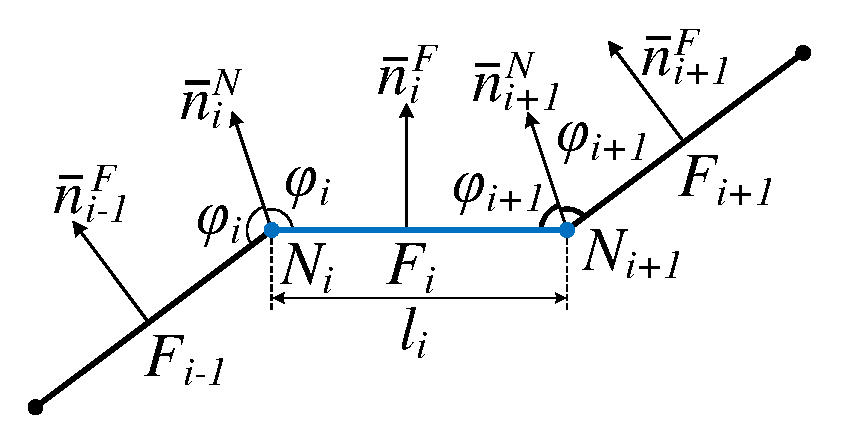
\includegraphics[width=0.75\columnwidth]{fig/2dr_grid_normals_big.pdf}\caption{обозначения}\end{subfigure} &
\begin{subfigure}{0.45\textwidth}\centering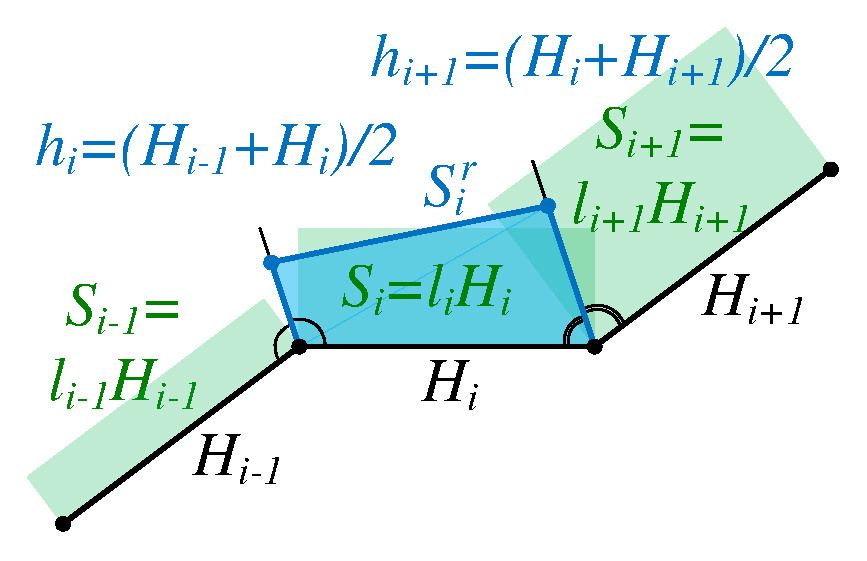
\includegraphics[width=0.75\columnwidth]{fig/2dr_remesh_rectangles_big.pdf}\caption{метод прямоугольников}\end{subfigure} \\
\begin{subfigure}{0.45\textwidth}\centering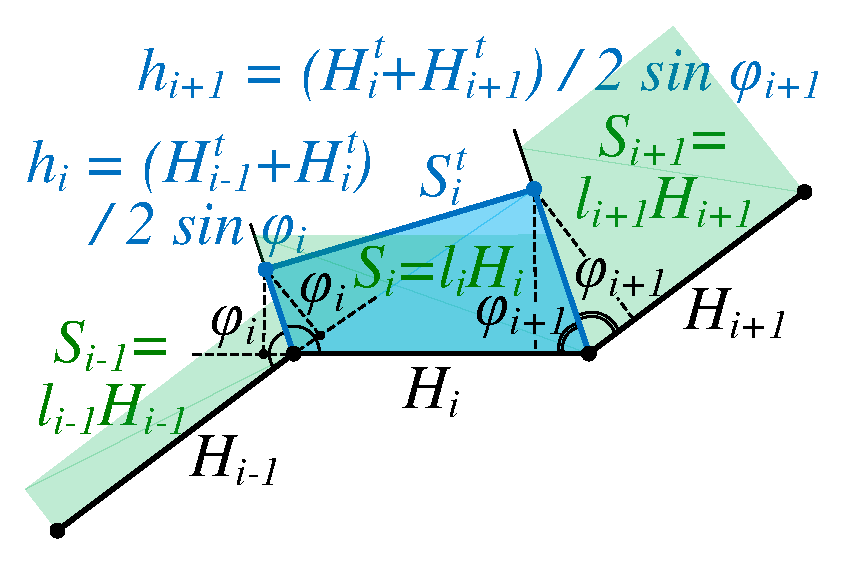
\includegraphics[width=0.75\columnwidth]{fig/2dr_remesh_trapeziums_big.pdf}\caption{метод трапеций}\end{subfigure} &
\begin{subfigure}{0.45\textwidth}\centering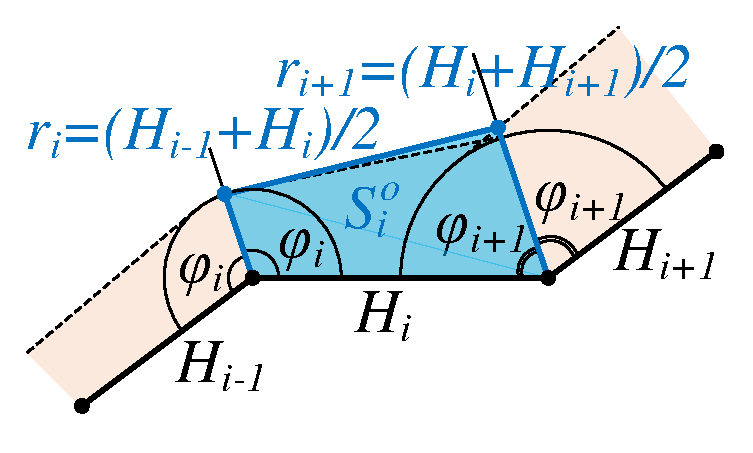
\includegraphics[width=0.75\columnwidth]{fig/2dr_remesh_okrestnost_big.pdf}\caption{метод окрестностей}\end{subfigure}
\end{tabular}
\singlespacing
\caption{Перестроение двумерной поверхностной сетки.}
\label{fig:remesh_2d}
\end{figure}

Для моделирования ледообразования центральной задачей перестроения поверхностной сетки является определение новых положений узлов $N'_i$, при которых площадь $S_i = S_{N_iN'_iN'_{i+1}N_{i+1}}$, заметаемая ячейкой $F_i$, как можно меньше отличается от \textit{целевой площади} $T_i = l_i H_i$, где $H_i$ -- вычисленная высота ледяного покрова в ячейке $F_i$.
Задача рассматривается при фиксированных направлениях смещения узлов $\overline{n}_i^N$, то есть требуется определить только величины смещения узлов $h_i$.
Для оценки абсолютного и относительного отклонения заметаемой площади от целевой используются обозначения $\Delta_i = S_i - T_i$, $\delta_i = \Delta_i / T_i$.

%----------------------------------

В разделе~1.1 определение величин смещений узлов $h_i$ рассматривается в общем виде, приводится вычисление заметаемой площади $S_i$ при движении ячейки и способ нахождения величин $h_i$ с помощью метода градиентного спуска нахождения минимума функции
\begin{equation*}
	D(\overline{h}) = \sum_{i = 0}^{n - 1}{\Delta_i^2} = \sum_{i = 0}^{n - 1}{ \left( \frac{ l_i(h_i \sin \phi_i + h_{i + 1} \sin \phi_{i+1}) - h_ih_{i + 1} \sin(\phi_i + \phi_{i+1}) }{2} - T_i \right)^2}
\end{equation*}

Так как решение задачи о перестроении сетки методом градиентного спуска оказывается слишком требовательным к вычислительным ресурсам, а качество решения зачастую оказывается неудовлетворительным при попадании в локальные минимумы, то делается вывод о необходимости рассмотрения приближенных методов перестроения.

%----------------------------------

В разделе~1.2 рассматриваются приближенные методы перестроения поверхностной сетки, основанные на представлении целевой площади с помощью примитивных геометрических фигур.

В первом методе (называемом \textit{методом прямоугольников}) целевая площадь для $i$-ой ячейки представлена прямоугольником со сторонами $l_i$ и $H_i$, и величина смещения узла определяется как $h_i = (H_{i - 1} + H_i)/2$ (рис.~\ref{fig:remesh_2d}~б).

В качестве второго метода рассматривается \textit{метод трапеций} (рис.~\ref{fig:remesh_2d}~в), в котором целевая площадь для $i$-ой ячейки представлена трапецией с площадью $T_i$ и боковыми сторонами, лежащими на направлениях $\overline{n}_i^N$, $\overline{n}_{i + 1}^N$, высота этой трапеции обозначена $H_i^t$.
После построения трапеций для всех ячеек сетки у каждого узла появляются две новые потенциальные позиции для сдвига (образованные ячейкой слева и ячейкой справа).
В качестве финальной новой позиции выбирается их среднее значение, и $h_i = (H_{i - 1}^t + H_i^t) / (2 \sin \phi_i)$.

Предлагается новый метод перестроения, называемый \textit{методом окрестностей}.
\textit{Окрестностью} множества точек $G$ называется множество $O_R(G) = \{ P: \exists C \in G \implies P \in Ball(C, R(C)) \}$, где $R: G \rightarrow \mathbb{R}_{\ge 0}$ -- заданная функция, а $Ball(C, R)$ -- шар с центром в $C$ и радиусом $R$.
В методе окрестностей в качестве нового положения узла $N'_i$ берется пересечение направления $\overline{n}_i^N$ и границы окрестности ячеек, инцидентных узлу $N_i$.

%----------------------------------

В разделе~1.3 приводится аналитическая оценки точности приближенных методов перестроения.
Оценка проводится для модельной расчетной сетки, удовлетворяющей следующим требованиям: все ячейки имеют длину $l$, для любой ячейки $N_iN_{i + 1} = AB$ и ее соседей $N_{i - 1}A$ и $BN_{i + 2}$ верно $\angle (\overline{BA}, \overline{AN_{i - 1}}) = \angle (\overline{AB}, \overline{BN_{i + 2}}) = \alpha$ (для выпуклой сетки полагаем $\alpha \ge 0$, для вогнутой $\alpha < 0$).
Высоты накопленного слоя льда в ячейках $N_{i - 1}A$, $AB$ и $BN_{i + 2}$ принимаются равными $H_{i - 1}$, $H_i$ и $H_{i + 1}$ соответственно.
Имеет место линейное изменение высоты накопленного льда, то есть $H_i - H_{i - 1} = H_{i + 1} - H_i = \Delta H$.
Величины смещения узлов при перестроении сетки равны $h_i$, $h_{i + 1}$.
В этих предположениях справедлива следующая лемма.

\textbf{Лемма.} \textit{Для ячейки модельной рачетной сетки площадь, заметаемая $i$-ой ячейкой, равна $S_i = \frac{1}{2} \sin \alpha \left( \lambda(h_i + h_{i+1}) + h_ih_{i+1} \right)$, где $\lambda = l / (2 \sin \frac{\alpha}{2})$.}

\begin{figure}[ht]
\centering
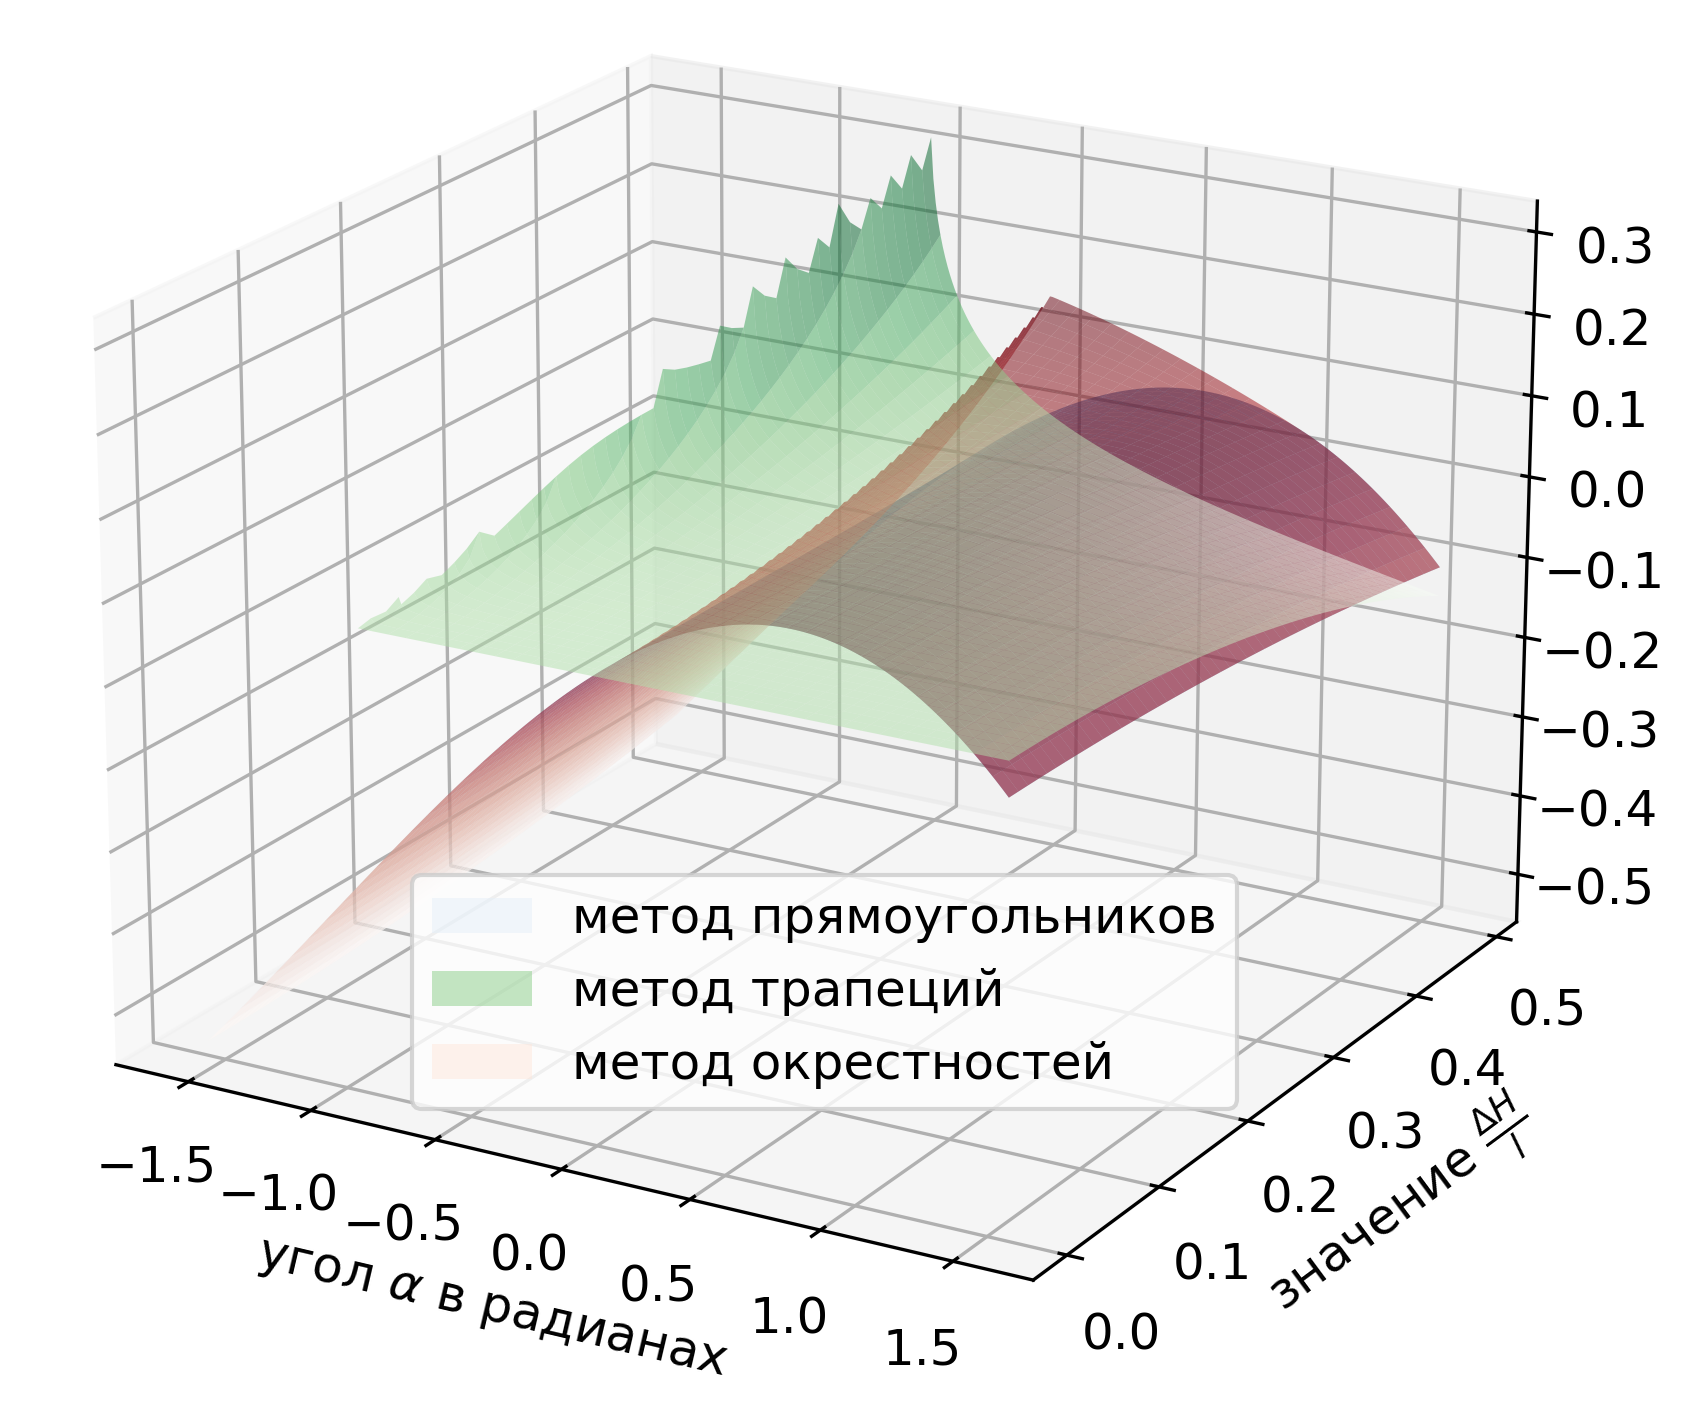
\includegraphics[width=0.6\textwidth]{fig/2dr_remesh_3d_chart_big.png}
\singlespacing
\caption{Графики $\delta_i^r(\alpha, \frac{\Delta H}{l})$, $\delta_i^t(\alpha, \frac{\Delta H}{l})$, $\delta_i^o(\alpha, \frac{\Delta H}{l})$ при $H = \frac{l}{2}$.}
\label{fig:text_1_remesh_3d_main_chart}
\end{figure}

На основе леммы для рассмотренных методов перестроения получены выражения для $h_i$ в аналитическом виде, получены зависимости относительных отклонений заметаемой площади от целевой $\delta_i^r(\alpha, \frac{\Delta H}{l})$, $\delta_i^t(\alpha, \frac{\Delta H}{l})$, $\delta_i^o(\alpha, \frac{\Delta H}{l})$ для методов прямоугольников, трапеций и окрестностей соответственно и проведен их анализ, представленный на рис.~\ref{fig:text_1_remesh_3d_main_chart}.
Полученные оценки показали, что при $\Delta H = 0$ метод трапеций абсолютно точен.
Также из построенных графиков можно отметить, что при $\Delta H$ близких к нулю отклонения $\delta_i^r$ и $\delta_i^o$ отличаются слабо.
На рис.~\ref{fig:text_1_remesh_fix_alfa_chart} дополнительно приведены срезы поверхностей $\delta_i^r(\alpha, \frac{\Delta H}{l})$, $\delta_i^t(\alpha, \frac{\Delta H}{l})$, $\delta_i^o(\alpha, \frac{\Delta H}{l})$ при фиксированных значениях $\alpha \pm 0,5$, на которых видно, что при блюзких к нулю значениях $\Delta H$ метод трапеций является наиболее точным, а методы прямоугольников и окрестностей демонстрируют близкие результаты.

\begin{figure}[ht]
\centering
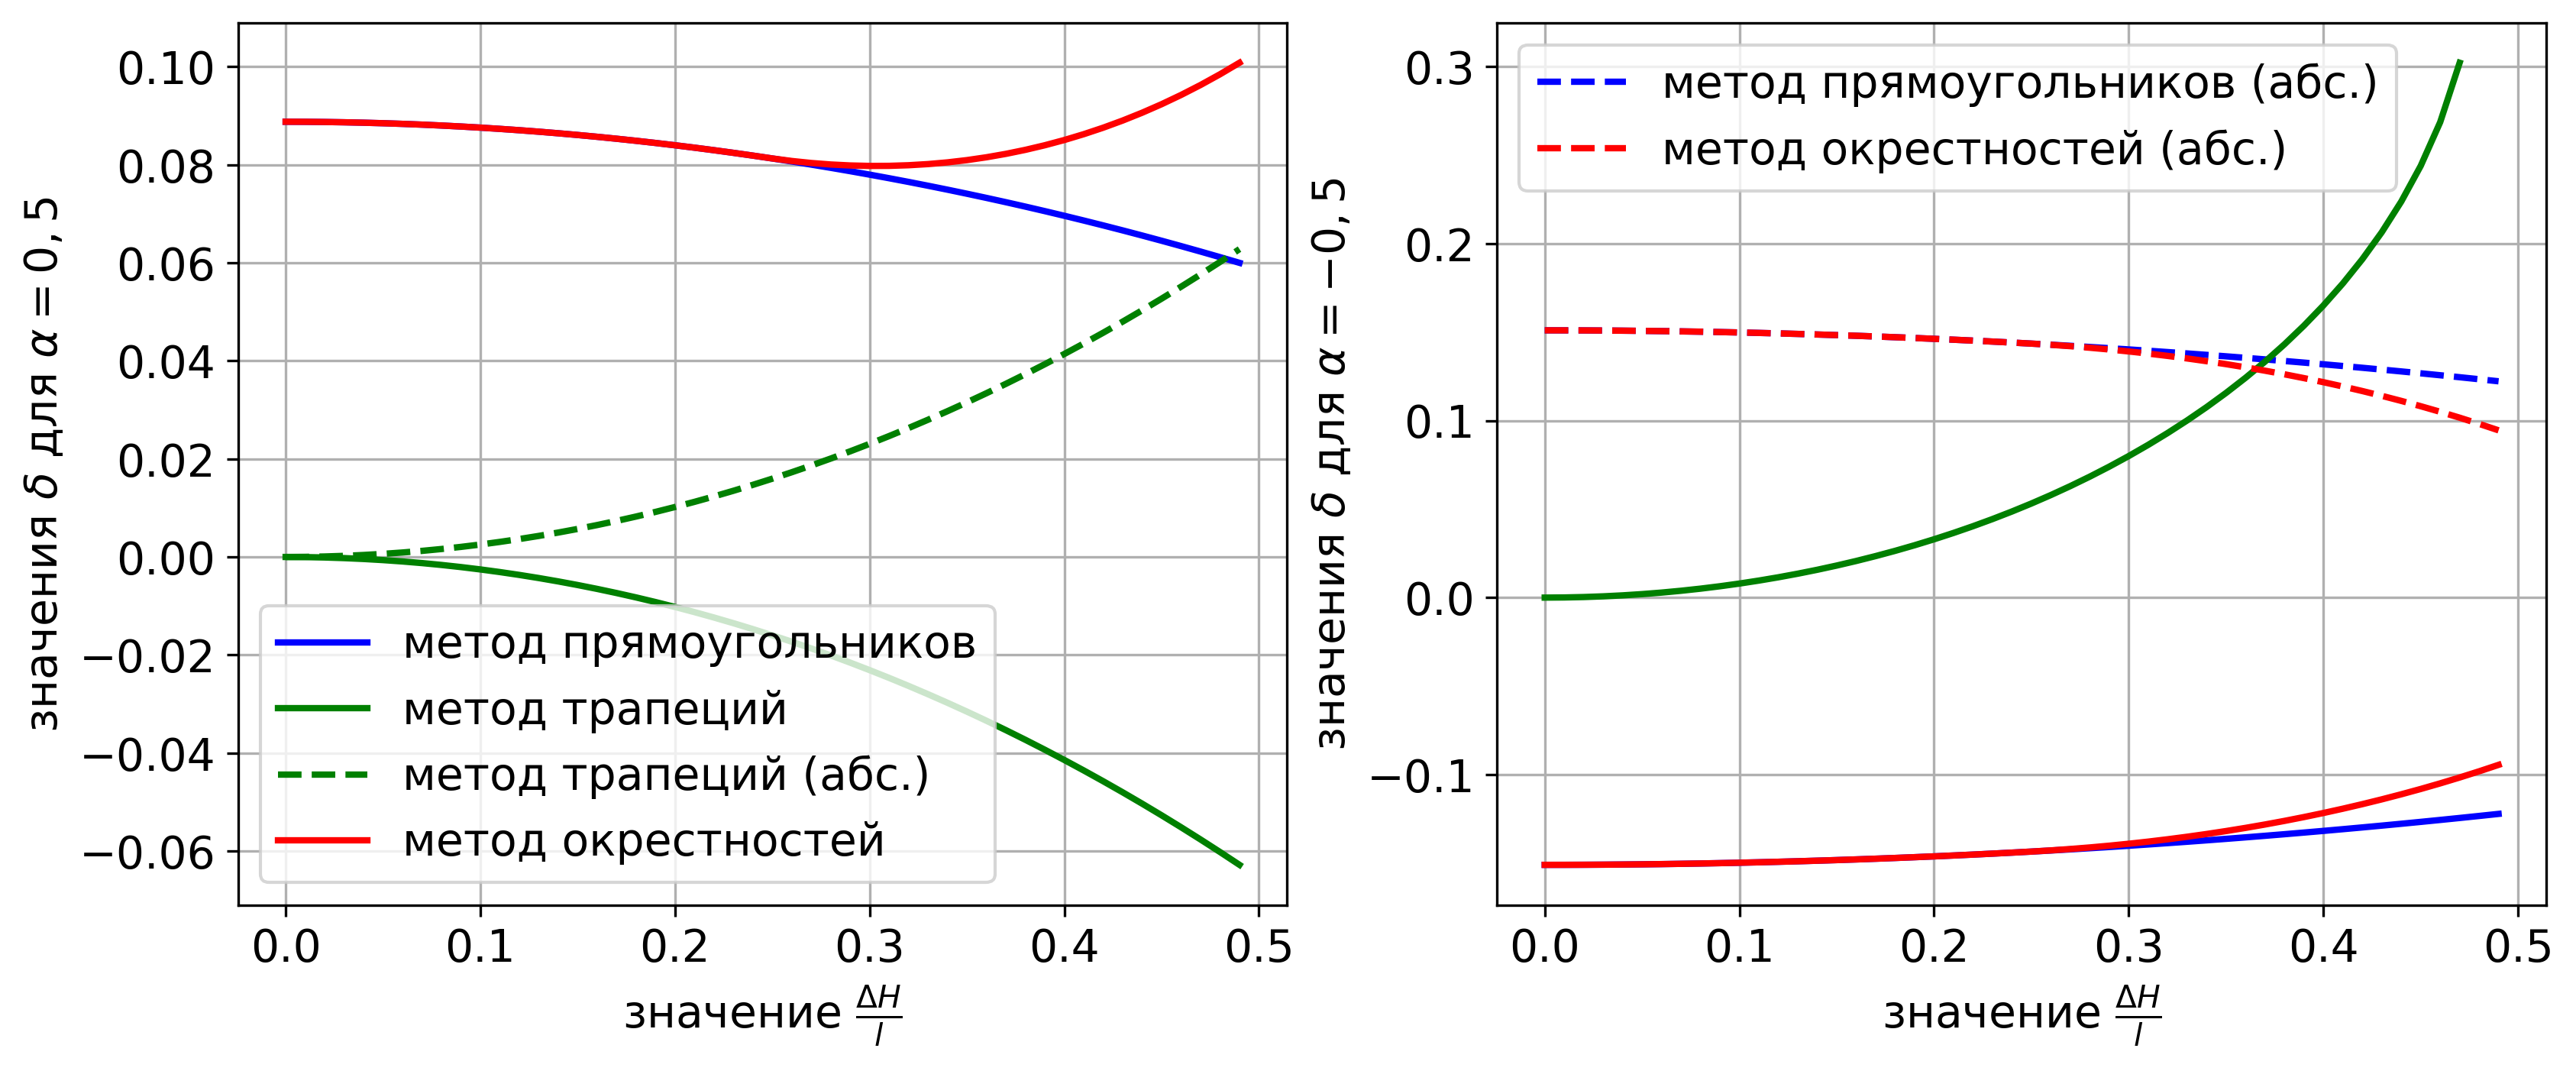
\includegraphics[width=0.8\textwidth]{fig/2dr_remesh_fix_alfa_chart_big.png}
\singlespacing
\caption{Графики $\delta_i^r(\frac{\Delta H}{l})$, $\delta_i^t(\frac{\Delta H}{l})$, $\delta_i^o(\frac{\Delta H}{l})$ при $\alpha = \pm 0,5$.}
\label{fig:text_1_remesh_fix_alfa_chart}
\end{figure}

%----------------------------------

В разделе~1.4 приведены оценки сглаживания дефектов сетки, таких как острые пики и впадины, для рассмотренных методов перестроения.
Для оценки сглаживания острых пиков считается, что сетка является абсолютно плоской за исключением двух соседних ячеек, которые образуют острый пик с углом $2 \alpha$.
Для оценки сглаживания впадин считается, что сетка является абсолютно плоской за исключением двух соседних ячеек, которые образуют впадину с углом $2 \alpha$.
Для оценок сглаживания углов дефектов сетки справедливы следующие леммы.

\textbf{Лемма.} \textit{Сглаженный угол при остром пике выражается как $\hat{\alpha}(h_A, h_B) = \arctg \frac{l \sin \alpha + h_B \cos \gamma}{l \cos \alpha + h_A - h_B \sin \gamma}$, где $A$ -- вершина острого пика, $B$ -- ее соседний узел, а $h_A$ и $h_B$ -- смещения этих узлов при перестроении сетки.}

\textbf{Лемма.} \textit{Сглаженный угол при впадине выражается как $\check{\alpha}(h_A, h_B) = \arctg \frac{l \sin \alpha - h_B \cos \gamma}{l \cos \alpha - h_A + h_B \sin \gamma}$ при условии $\arcsin \frac{h_B ( \sqrt{8 l^2 + h_B^2} - h_B )}{4 l^2} \le \alpha \le \arccos \frac{h_A}{l}$, где $A$ -- вершина спадины, $B$ -- ее соседний узел, а $h_A$ и $h_B$ -- смещения этих узлов при перестроении сетки.}


\begin{figure}[ht]
\centering
\begin{tabular}{l}
\begin{subfigure}{0.9\textwidth}\centering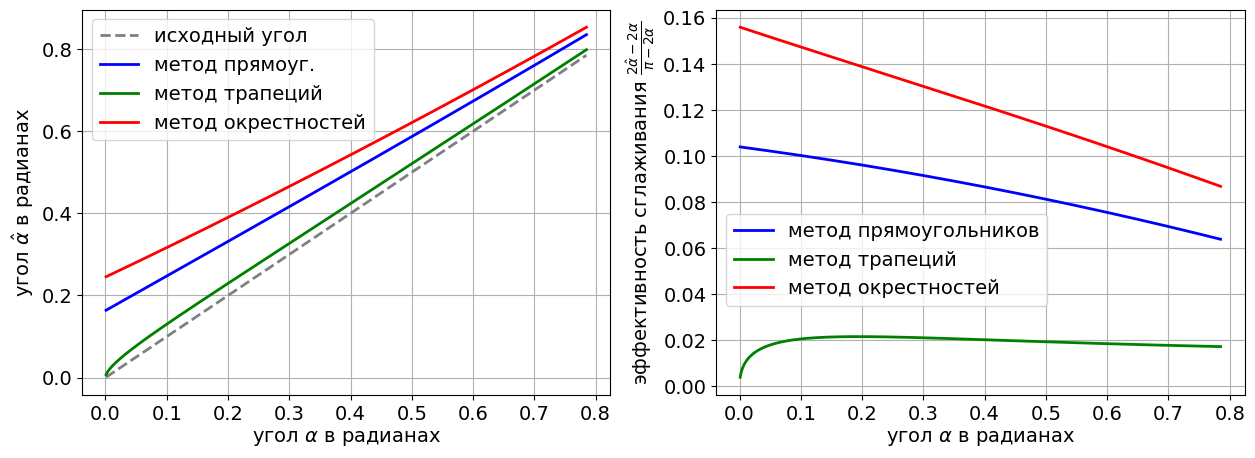
\includegraphics[width=1.0\columnwidth]{fig/2dr_peak_methods_chart_big.png}\caption{сглаживание угла при остром пике}\end{subfigure} \\
\begin{subfigure}{0.9\textwidth}\centering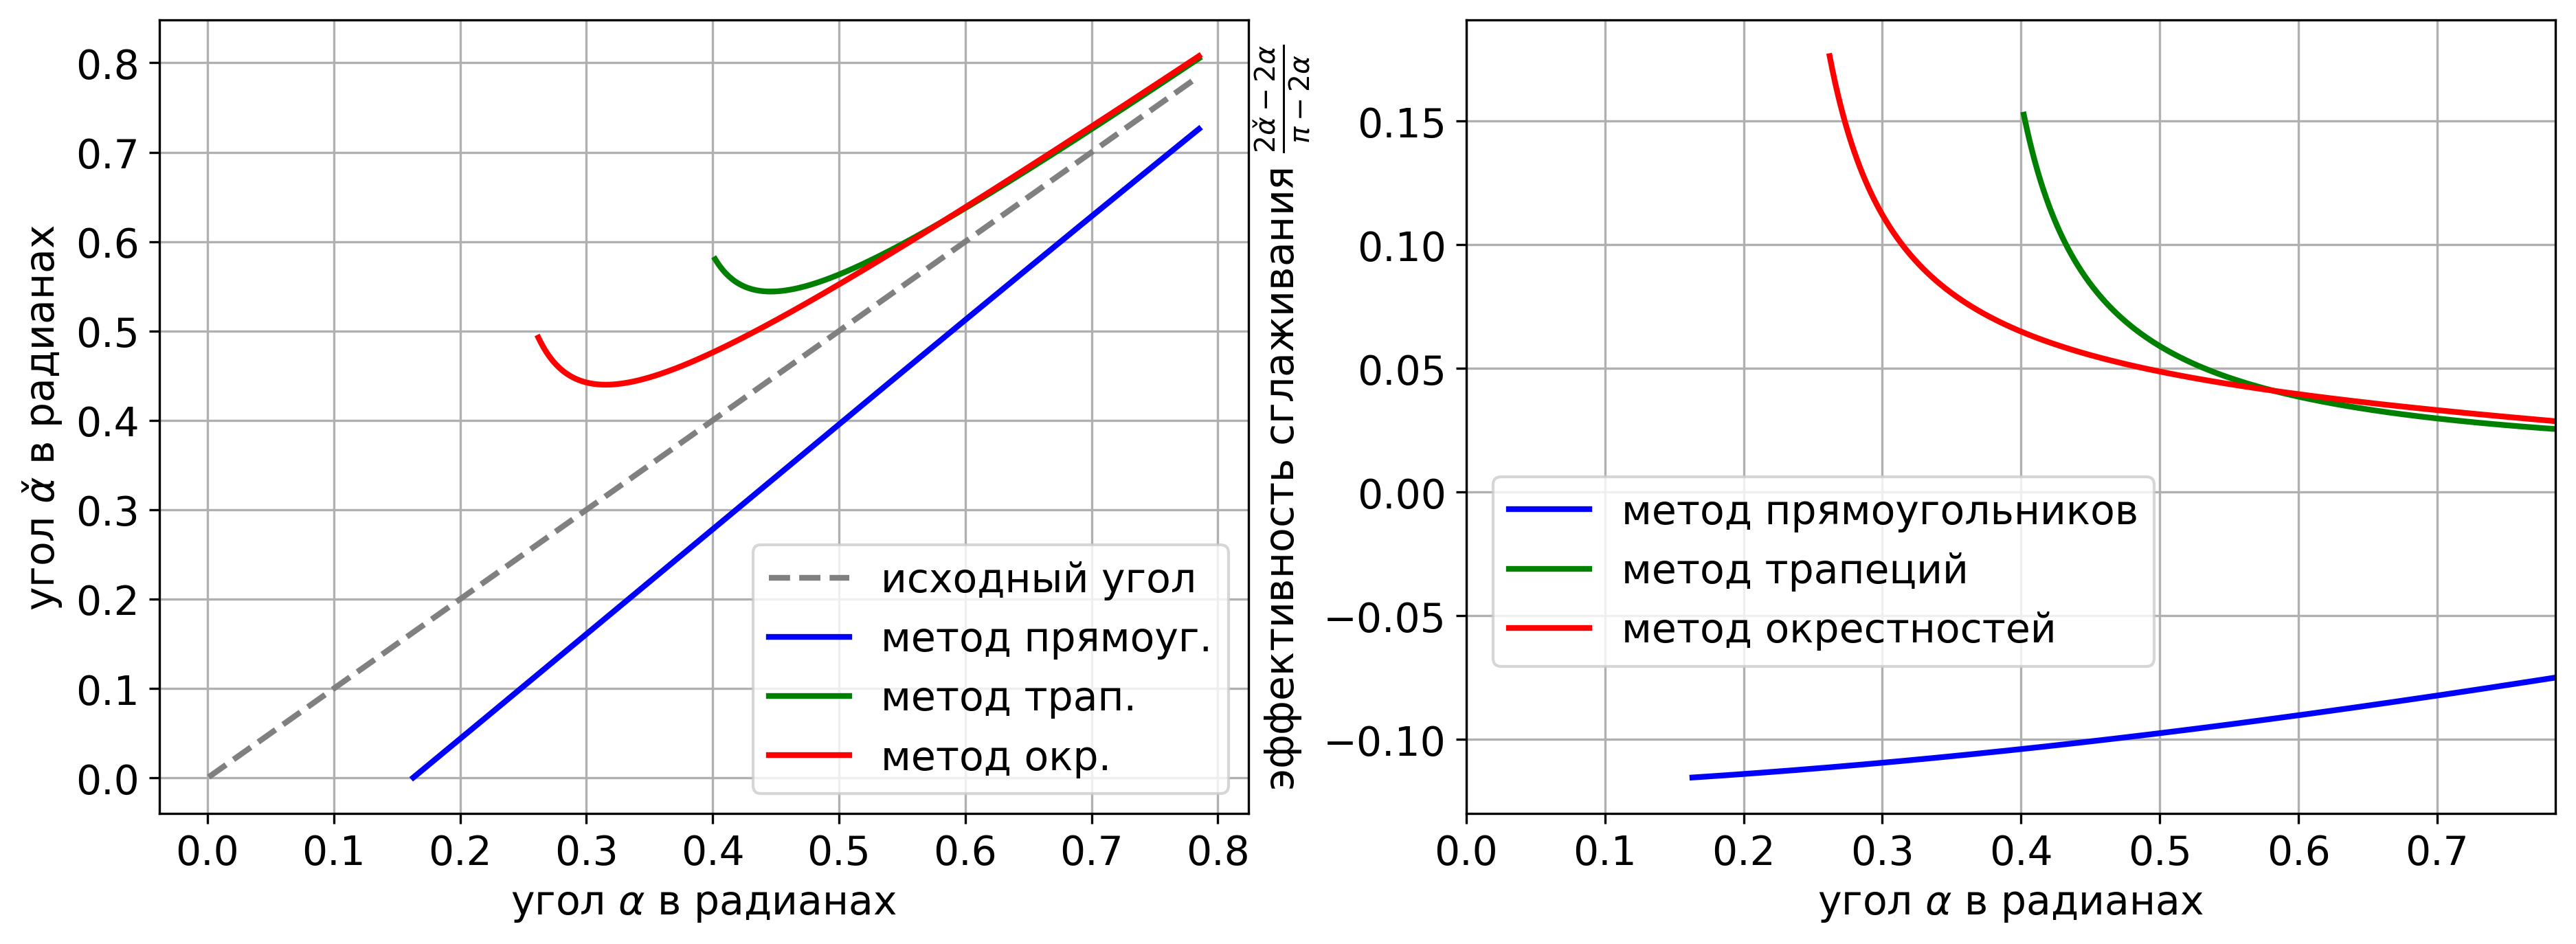
\includegraphics[width=1.0\columnwidth]{fig/2dr_cavern_methods_chart_big.png}\caption{сглаживание угла при впадине}\end{subfigure}
\end{tabular}
\singlespacing
\caption{Сравнение сглаживания углов при дефектах сетки.}
\label{fig:smooth_2d}
\end{figure}

На рис.~\ref{fig:smooth_2d} сверху приведены графики сравнения методов перестроения в применении к сглаживанию острых пиков при $H = \frac{l}{4}$.
Слева показана зависимость изменения сглаженного угла $\hat{\alpha}$ от $\alpha$, справа -- \textit{эффективность сглаживания}, выраженная формулой $\frac{2 \hat{\alpha} - 2 \alpha}{\pi - 2 \alpha}$ (значение 1 означает полное сглаживание пика до угла $\hat{\alpha} = \frac{\pi}{2}$).
Наиболее эффективное сглаживание угла $\alpha$ обеспечивает метод окрестностей.
Использование метода трапеций для малых углов $\alpha$ приводит к неконтролируемому росту $h_A$, что делает применение этого метода неприемлемым.

На рис.~\ref{fig:smooth_2d} снизу приведены графики сравнения методов перестрения в применении к сглаживанию впадин при $H = \frac{l}{4}$.
Слева показана зависимость изменения сглаженного угла $\check{\alpha}$ от $\alpha$, справа -- эффективность сглаживания.
Из графиков видно, что метод прямоугольников не сглаживает угол, а наоборот, делает его еще более острым (значение эффективности сглаживания меньше нуля).
Метод трапеций показывает лучшую эффективность сглаживания, но с меньшей областью применимости.

В выводах к главе отмечено, что метод окрестностей перестроения поверхностной расчетной сетки является наиболее подходящим для моделирования ледообразования с точки зрения точности перестроения и эффективности сглаживания дефектов.
Метод окрестностей по точности перестроения близок к методу прямоугольников, а также позволяет сглаживать как острые пики, так и впадины сетки.
Эффективность сглаживания дефектов сетки обеспечивает стабильность вычислений.

%---------------------------------------------------------------------------------------------------

\textbf{Вторая глава} посвящена исследованию перестроения поверхностной расчетной сетки в трехмерном случае, рассматриваются известные методы и предлагается обобщение предложенного метода окрестностей перестроения расчетной сетки на трехмерный случай.
Расчетная сетка описывает двустороннюю поверхность без самопересечений, каждое ребро которой имеет не более двух инцидентных ячеек.
Для ячеек $F$ определены внешние единичные нормали $\overline{n}_F^F$, через которые для узлов $N$ также определены внешние единичные нормали $\overline{n}_N^N = \sum_{F \in \mathscr{F}(N)}{\overline{n}_F^F} / |\sum_{F \in \mathscr{F}(N)}{\overline{n}_F^F}|$ по аналогии с двумерным случаем, где $\mathscr{F}(N)$ -- инцидентные $N$ ячейки.

%----------------------------------

В разделе~2.1 рассматриваются классические методы перестроения при фиксированных направлениях смещения узлов $\overline{n}^N$ (рис.~\ref{fig:text_1_remesh3}).
В каждой ячейке $F = ABC$ известен объем накопленного льда $V_F$, для каждого узла $N$ требуется найти новое положение $N'$, чтобы объем пространства, ограниченный фигурой $ABCA'B'C'$ соответствовал объему накопленного льда $V_F$.
Таким образом, поставновка задачи в трехмерном случае аналогично двумерной постановке.

\begin{figure}[h]
\centering
\begin{tabular}{ll}
\begin{subfigure}{0.4\textwidth}\centering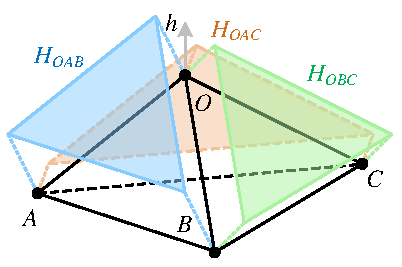
\includegraphics[width=1.0\columnwidth]{fig/3dr_prisms_big.pdf}\caption{метод призм}\end{subfigure} &
\begin{subfigure}{0.45\textwidth}\centering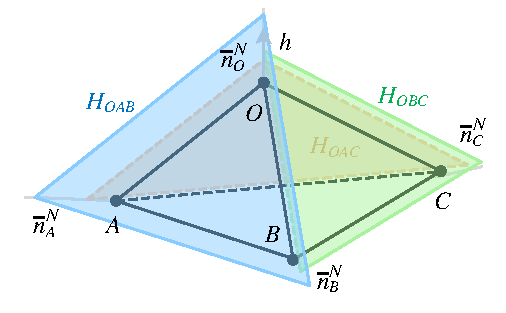
\includegraphics[width=1.0\columnwidth]{fig/3dr_pyramids_big.pdf}\caption{метод пирамид}\end{subfigure}
\end{tabular}
\singlespacing
\caption{Перестроение поверхностной сетки с трехмерном случае.}
\label{fig:text_1_remesh3}
\end{figure}

В \textit{методе призм} (аналог двумерного метода прямоугольников) в качестве приближения целевого объема рассматривается призма, одним из оснований которой является ячейка.
В \textit{методе пирамид} (аналог двумерного метода трапеций) в качестве приближения целевого объема рассматривается призматоид, одним из оснований которого является ячейка, а боковые стороны направлены вдоль направлений смещения узлов.

В разделе рассматриваются дополнительные аспекты перестроения поверхностной сетки, в которых $\overline{n}^N$ могут менять свое направление.
В частности рассматривается многослойный метод перестроения, в котором выполнятеся $k$ последовательных шагов перестроения сетки, на каждом из которых решается задача для объема накопленного в ячейке $F$ льда в количестве $V_F/k$.
Рассматриваются метод сглаживания поля нормалей $\overline{n}^N$, $\overline{n}^F$ для предотвращения раннего самопересечения сетки, метод сглаживания высот льда в ячейках для устранения поверхностного шума, а также метод сглаживания сетки, позволяющий перераспределить узлы по поверхности для получения более сбалансированного размера ячеек\footnote[1]{X.~Tong, D.~Thompson, Q.~Arnoldus, E.~Collins, E.~Luke. Three-dimensional surface evolution and mesh deformation for aircraft icing applications. // Journal of Aircraft, 2017, Vol.~54, P.~1047–1063, doi:~10.
2514/1.C033949}.

%----------------------------------

В разделе~2.2 приводится полное описания метода окрестностей перестроения поверхностной неструктурированной расчетной сетки в трехмерной постановке.
Рассматривается геометрическая задача определения новых положений узлов расчетной сетки, если для каждого узла $N$ известна скорость образования ледяного покрова $v_N$.
Нарастание льда в любой точке роста льда выполняется одновременно во всех направлениях аналогично принципу Гюйгенса-Френеля распространения волн.
Расчет новых положений узлов выполняется через некоторый фиксированный момент времени $\Delta t$, таким образом для каждого узла $N$ известен радиус \textit{области распространения льда} (ОРЛ) узла $R_N = v_N \Delta t$.
В методе окрестностей аналогично двумерному случаю в качестве нового положения узла $N'$ берется пересечение направления смещения узла $\overline{n}_N^N$ и границы окрестности всех инцидентных узлу ячеек $O_R$, где радиус ОРЛ внутренней точки $\overline{P}(\beta, \gamma) = \overline{A} + \beta (\overline{B} - \overline{A}) + \gamma (\overline{C} - \overline{A})$ ячейки $ABC$ определяется как $R(\overline{P}(\beta,\gamma)) = R(\beta,\gamma) = R_A + \beta(R_B - R_A) + \gamma(R_C - R_A) = R_A + \beta R_{AB} + \gamma R_{AC}$, где $\beta \ge 0$, $\gamma \ge 0$, $\beta + \gamma \le 1$.

Точка пересечения траектории движения узла $A$ ($\overline{P}(\alpha) = \overline{A} + \alpha \overline{D}$, где $\overline{D} = \overline{n}_A^N$ при $\alpha \ge 0$) с $O_R(ABC)$ -- это наибольший корень уравнения
\begin{equation*}
|(\overline{A} + \alpha \overline{D}) - \overline{P}(\beta, \gamma)| = R(\beta, \gamma)
\end{equation*}
относительно $\alpha$ при ограничениях $\beta \ge 0$, $\gamma \ge 0$, $\beta + \gamma \le 1$.
Наибольший корень этого уравнения при условии $|\overline{D}| = 1$ выражается следующим образом:
\begin{equation*}
	\begin{aligned}
		& \alpha(\beta, \gamma) = k_{\beta} \beta + k_{\gamma} \gamma + \sqrt{T} \\
		& T = q_{\beta^2} \beta^2 + q_{\gamma^2} \gamma^2 + q_{\beta \gamma} \beta \gamma + q_{\beta} \beta + q_{\gamma} \gamma + q \\
		& k_{\beta} = (\overline{D}, \overline{AB}), \ k_{\gamma} = (\overline{D}, \overline{AC}) \\
		& q_{\beta^2} = (\overline{D}, \overline{AB})^2 - |\overline{AB}|^2 + R_{AB}^2 \\
		& q_{\gamma^2} = (\overline{D}, \overline{AC})^2 - |\overline{AC}|^2 + R_{AC}^2 \\
		& q_{\beta \gamma} = 2 \left( (\overline{D}, \overline{AB}) (\overline{D}, \overline{AC}) - (\overline{AB}, \overline{AC}) + R_{AB}R_{AC} \right) \\
		& q_{\beta} = 2 R_A R_{AB}, \ q_{\gamma} = 2 R_A R_{AC}, \ q = R_A^2
	\end{aligned}
\end{equation*}

Для поиска нового положения узла $A$ относительно ячейки $ABC$ требуется найти максимум выражения $\alpha(\beta, \gamma)$ при условии соблюдения ограничений $\beta \ge 0$, $\gamma \ge 0$, $\beta + \gamma \le 1$ (соответствующее значение $\alpha$ обозначается $\alpha(ABC)$).
При рассмотрении узла сетки требуется вычислить смещение этого узла относительно каждой инцидентной ячейки и выбрать среди этих смещений максимальное, тогда $\overline{A}' = \overline{A} + \overline{n}_A^N \cdot \max_{F \in \mathscr{F}(A)}{\alpha(F)}$.

В методе окрестностей при нахождении значений $\alpha(F)$ не используются итерационные методы вычислений, поэтому алгоритм перестроения поверхностной сетки имеет линейную сложность по количеству узлов.

Предложенный метод окрестностей перестроения поверхностной неструктурированной расчетной сетки в трехмерном случае, также как и его двумерный аналог, обладает способностью сглаживания дефектов расчетной сетки при приемлемой точности перестроения.
В сочетании с многослойным подходом метод окрестностей позволяет избежать появления острых пиков и кромок во время моделирования ледообразования, а также приводит к затягиванию узких впадин и изломов (рис.~\ref{fig:text_1_remesh3_with_fensap}).
Свойство сглаживания дефектов является крайне важным, так как обеспечивает стабильность моделирования нарастания льда и позволяет отложить корректировку расчетной сетки вплоть до фазы устранения глобального дефекта -- самопересечения сетки.

\begin{figure}[!ht]
\centering
\begin{tabular}{ll}
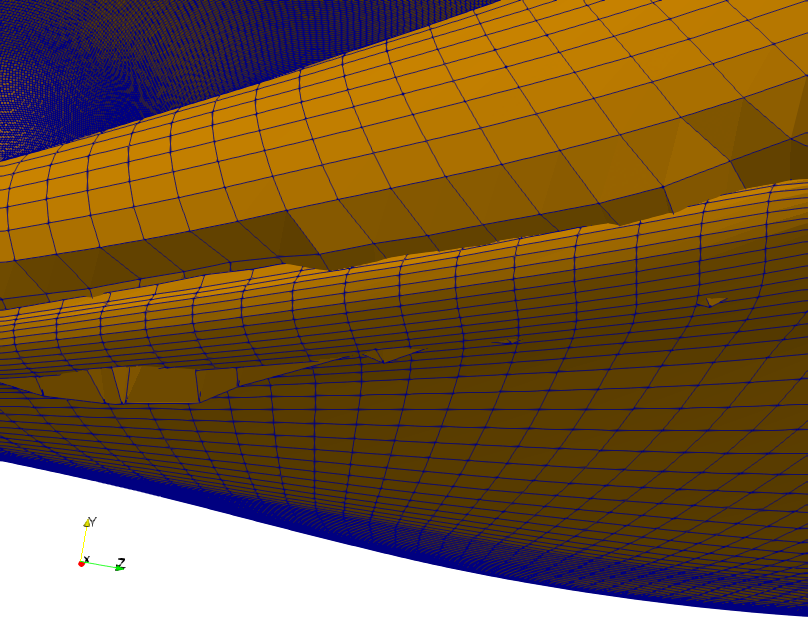
\includegraphics[width=0.43\textwidth]{fig/3dr_fens1.png}
&
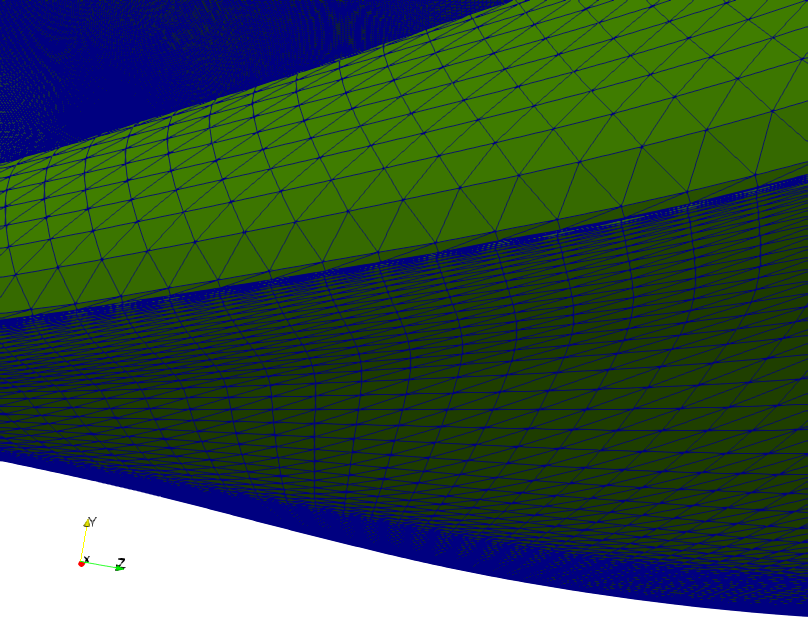
\includegraphics[width=0.43\textwidth]{fig/3dr_crys1.png} \\
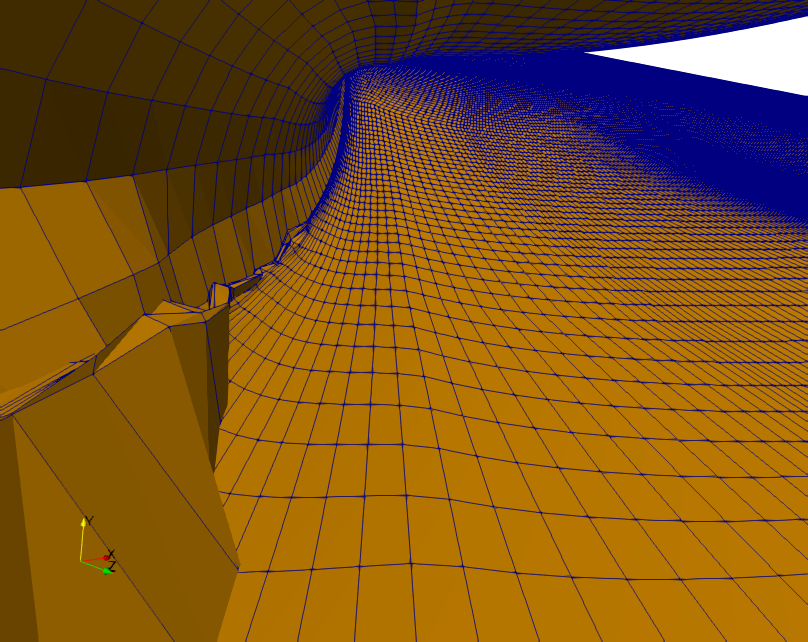
\includegraphics[width=0.43\textwidth]{fig/3dr_fens2.png}
&
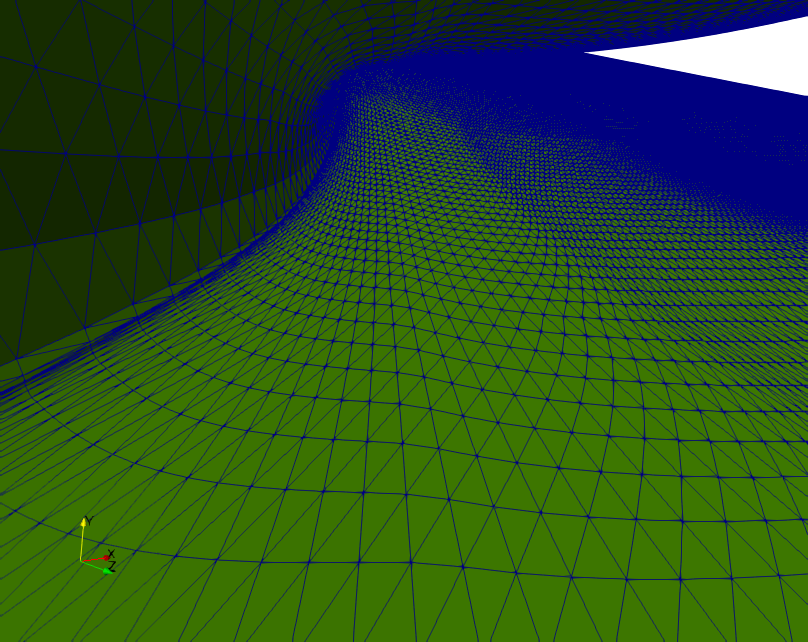
\includegraphics[width=0.43\textwidth]{fig/3dr_crys2.png}
\end{tabular}
\singlespacing
\caption{Эффект сглаживания дефектов при перестроении методом окрестностей (справа) в сравнении с программным комплексом FENSAP-ICE (слева).}
\label{fig:text_1_remesh3_with_fensap}
\end{figure}

В выводах к главе отмечено, что метод окрестностей перестроения поверхностной расчетной сетки в трехмерной постановке позволяет сглаживать дефекты, что обеспечивает стабильное перестроение в процессе моделирования ледообразования.
Линейная сложность алгоритма позволила использовать его для промышленных расчетов.

%---------------------------------------------------------------------------------------------------

\textbf{Третья глава} посвящена исследованию корректировки поверхностной расчетной сетки после перестроения.
Исследуется проблема удаления самопересечений поверхностной сетки, анализируются существующие методы, предлагаются новые методы удаления самопересечений.
Исследуется проблема сопряжения с объемной расчетной сеткой, возникающая после перестроения поверхностной сетки.

В разделе~3.1 рассматривается проблема удаления самопересечений поверхностной неструктурированной расчетной сетки.
В общем случае предотвратить возникновение самопересечений невозможно, так как в процессе ледообразования при активном нарастании льда возможно взаимное пересечение ледяных наростов.
Самопересечение является критическим дефектом сетки, при котором невозможно производить дальнейшие вычисления по моделированию ледообразования, поэтому самопересечения необходимо удалять.

\begin{figure}[!ht]
\centering
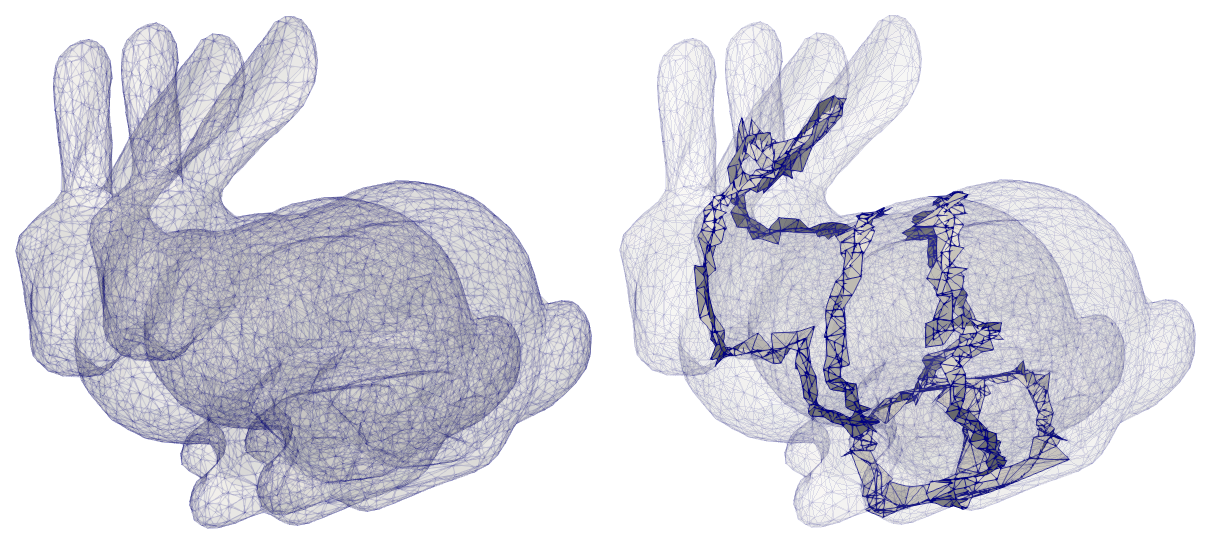
\includegraphics[width=1.0\textwidth]{fig/int_bunnies_dbl.png}
\singlespacing
\caption{Поиск пар пересекающихся ячеек.}
\label{fig:text_1_int_1}
\end{figure}

Предлагаются два подхода к удалению самопересечений.
Первый подход основан на разбиении ячеек на более мелкие по множествам точек и отрезков пересечения с другими ячейками.
Для этого сначала требуется найти все пары пересекающихся ячеек сетки (рис.~\ref{fig:text_1_int_1}), причем вариант непосредственной проверки всех пар треугольников на пересечение не является подходящим из-за высокой вычислительной сложности.

Для поиска пар пересекающихся треугольников используется \textit{дерево облаков треугольников} -- иерархическая структура, позволяющая избегать проверки на пересечение каждой пары.
Для построения дерева облаков треугольков используется понятие \textit{контейнера множества точек} $M$ -- наименьшего прямоугольного параллелепипеда, содержащего все эти точки:
\begin{equation*}
[M] = Box \left( \left[\min_{P \in M}{P_x}, \max_{P \in M}{P_x}\right],
                 \left[\min_{P \in M}{P_y}, \max_{P \in M}{P_y}\right],
                 \left[\min_{P \in M}{P_z}, \max_{P \in M}{P_z}\right] \right)
\end{equation*}
Контейнером треугольника является контейнер его вершин $[ABC] = [\{ABC\}]$.
Два треугольника называются \textit{потенциально пересекающимися}, если пересекаются их контейнеры.
Для контейнера множества треугольников можно определить \textit{дочерние контейнеры} таким образом, чтобы множество треугольников во всех дочерних контейнерах совпадало с множеством треугольников родительского контейнера.
Определим поиск всех пар потенциально пересекащихся треугольников, для этого введем следующие обозначения.
Пусть $M$ и $M'$ -- два множества треугольников, $K = [M]$ и $K' = [M']$ -- их контейнеры.
Обозначим через $\mathscr{P}(K, K')$ множество пар потенциально пересекающихся треугольников $(T, T')$ таких, что $T \in M$, $T' \in M'$.
Через $\mathscr{C}(K)$ обозначим множество дочерних контейнеров для контейнера $K$.
Тогда множество пар потенциально пересекающихся треугольников может быть вычислено рекурсивно как
\begin{equation*}
	\mathscr{P}(K, K') =
	\begin{cases}
		\bigcup_{ \substack{ L \in \mathscr{C}(K) \\ L' \in \mathscr{C}(K') } }{ \mathscr{P}(L, L') }, & \text{если } \mathscr{C}(K) \ne \emptyset, \ \mathscr{C}(K') \ne \emptyset \\
		\bigcup_{ L \in \mathscr{C}(K) }{ \mathscr{P}(L, K') },                                        & \text{если } \mathscr{C}(K) \ne \emptyset, \ \mathscr{C}(K') = \emptyset \\
		\mathscr{P}(K', K),                                                                            & \text{если } \mathscr{C}(K) = \emptyset, \ \mathscr{C}(K') \ne \emptyset \\
		\setlength{\jot}{-1pt}
		\begin{split}
			\{ (T, T') : \ & T \in M, \ T' \in M', \\
			               & T \ne T', \ [T] \cap [T'] \ne \emptyset \}
		\end{split},                                                                                   & \text{если } \mathscr{C}(K) = \emptyset, \ \mathscr{C}(K') = \emptyset
	\end{cases}
\end{equation*}

Множество пар пересекающихся треугольников является подмножеством $\mathscr{P}(K, K')$, таким образом при построении бинарного дерева облаков треугольников со сбалансированным количеством элементов в дочерних контейнерах существенно сокращаются затраты на их нахождение.

Основной проблемой при поиске множества точек пересечения двух треугольников являются ошибки точности при работе с числами с плавающей точкой, из-за которых может быть принято ошибочное решение о пересечении или непересечении: попадание узла на ребро или на ячейку, пересечение двух ребер, наложение ячеек.
В некоторых случаях такие конфликты можно разрешить локальной коррекцией положения узлов, тогда множество точек пересечения любой пары треугольников либо пусто, либо является отрезком (такую сетку будем называть \textit{простой}).
В случае, если сетка не является простой, установление точек пересечения треугольников выполняется в рациональных координатах (такой подход более затратный по времени, но избавлен от ошибок точности).
После определения всех точек пересечения ячеек, все пересекающиеся ячейки сетки разбиваются на более мелкие ячейки по множеству точек и отрезков пересечения.
После дробления ячеек в сетке отсутствуют пересекающиеся ячейки, однако некоторые ребра в ней имеют по 4 инцидентные ячейки в случае простой сетки и произвольное количество в противном случае, из которых только две относятся к \textit{внешней поверхности}, а все другие -- к \textit{скрытой области} сетки, которая должна быть удалена.
Внешняя область сетки определяется путем обхода ячеек.
При переходе с некоторой ячейки $APQ$ через ребро $PQ$ с несколькими инцидентными ячейками необходимо выбрать одну (в случае четырех инцидентных ячеек одну из $BPQ$, $CPQ$, $DPQ$).
Для простой сетки в качестве следующей ячейки, которая войдет в результирующую внешнюю поверхность, выбирается ячейка $NPQ$, $N \in \{ B, C, D \}$, для которой значение функции $f(N) = (\overline{n}_{APQ}^F, \overline{ON})$ максимально, где $O$ -- основание высоты треугольника $NPQ$, опущенной из вершины $N$ (рис.~\ref{fig:int_walk} а).
В противном случае выбирается ячейка, для которой угол $\phi(A \rightarrow N)$ поворота ячейки $APQ$ вокруг ребра $PQ$ в направлении внешней нормали до совмещения с плоскостью $NPQ$ минимален (рис.~\ref{fig:int_walk} в).

\begin{figure}[ht]
\centering
\begin{tabular}{lll}
\begin{subfigure}{0.33\textwidth}\centering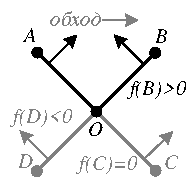
\includegraphics[width=0.6\columnwidth]{fig/int_walk_simple_big.pdf}\caption{простая сетка}\end{subfigure} &
\begin{subfigure}{0.33\textwidth}\centering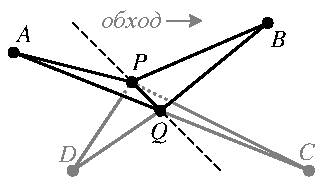
\includegraphics[width=0.7\columnwidth]{fig/int_walk_centre_big.pdf}\caption{схема обхода}\end{subfigure} &
\begin{subfigure}{0.33\textwidth}\centering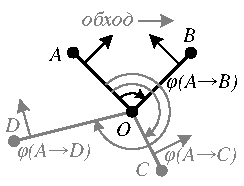
\includegraphics[width=0.7\columnwidth]{fig/int_walk_not_simple_big.pdf}\caption{общий случай}\end{subfigure}
\end{tabular}
\singlespacing
\caption{Обход внешней поверхности при устранении самопересечений.}
\label{fig:int_walk}
\end{figure}

\begin{figure}[!ht]
\centering
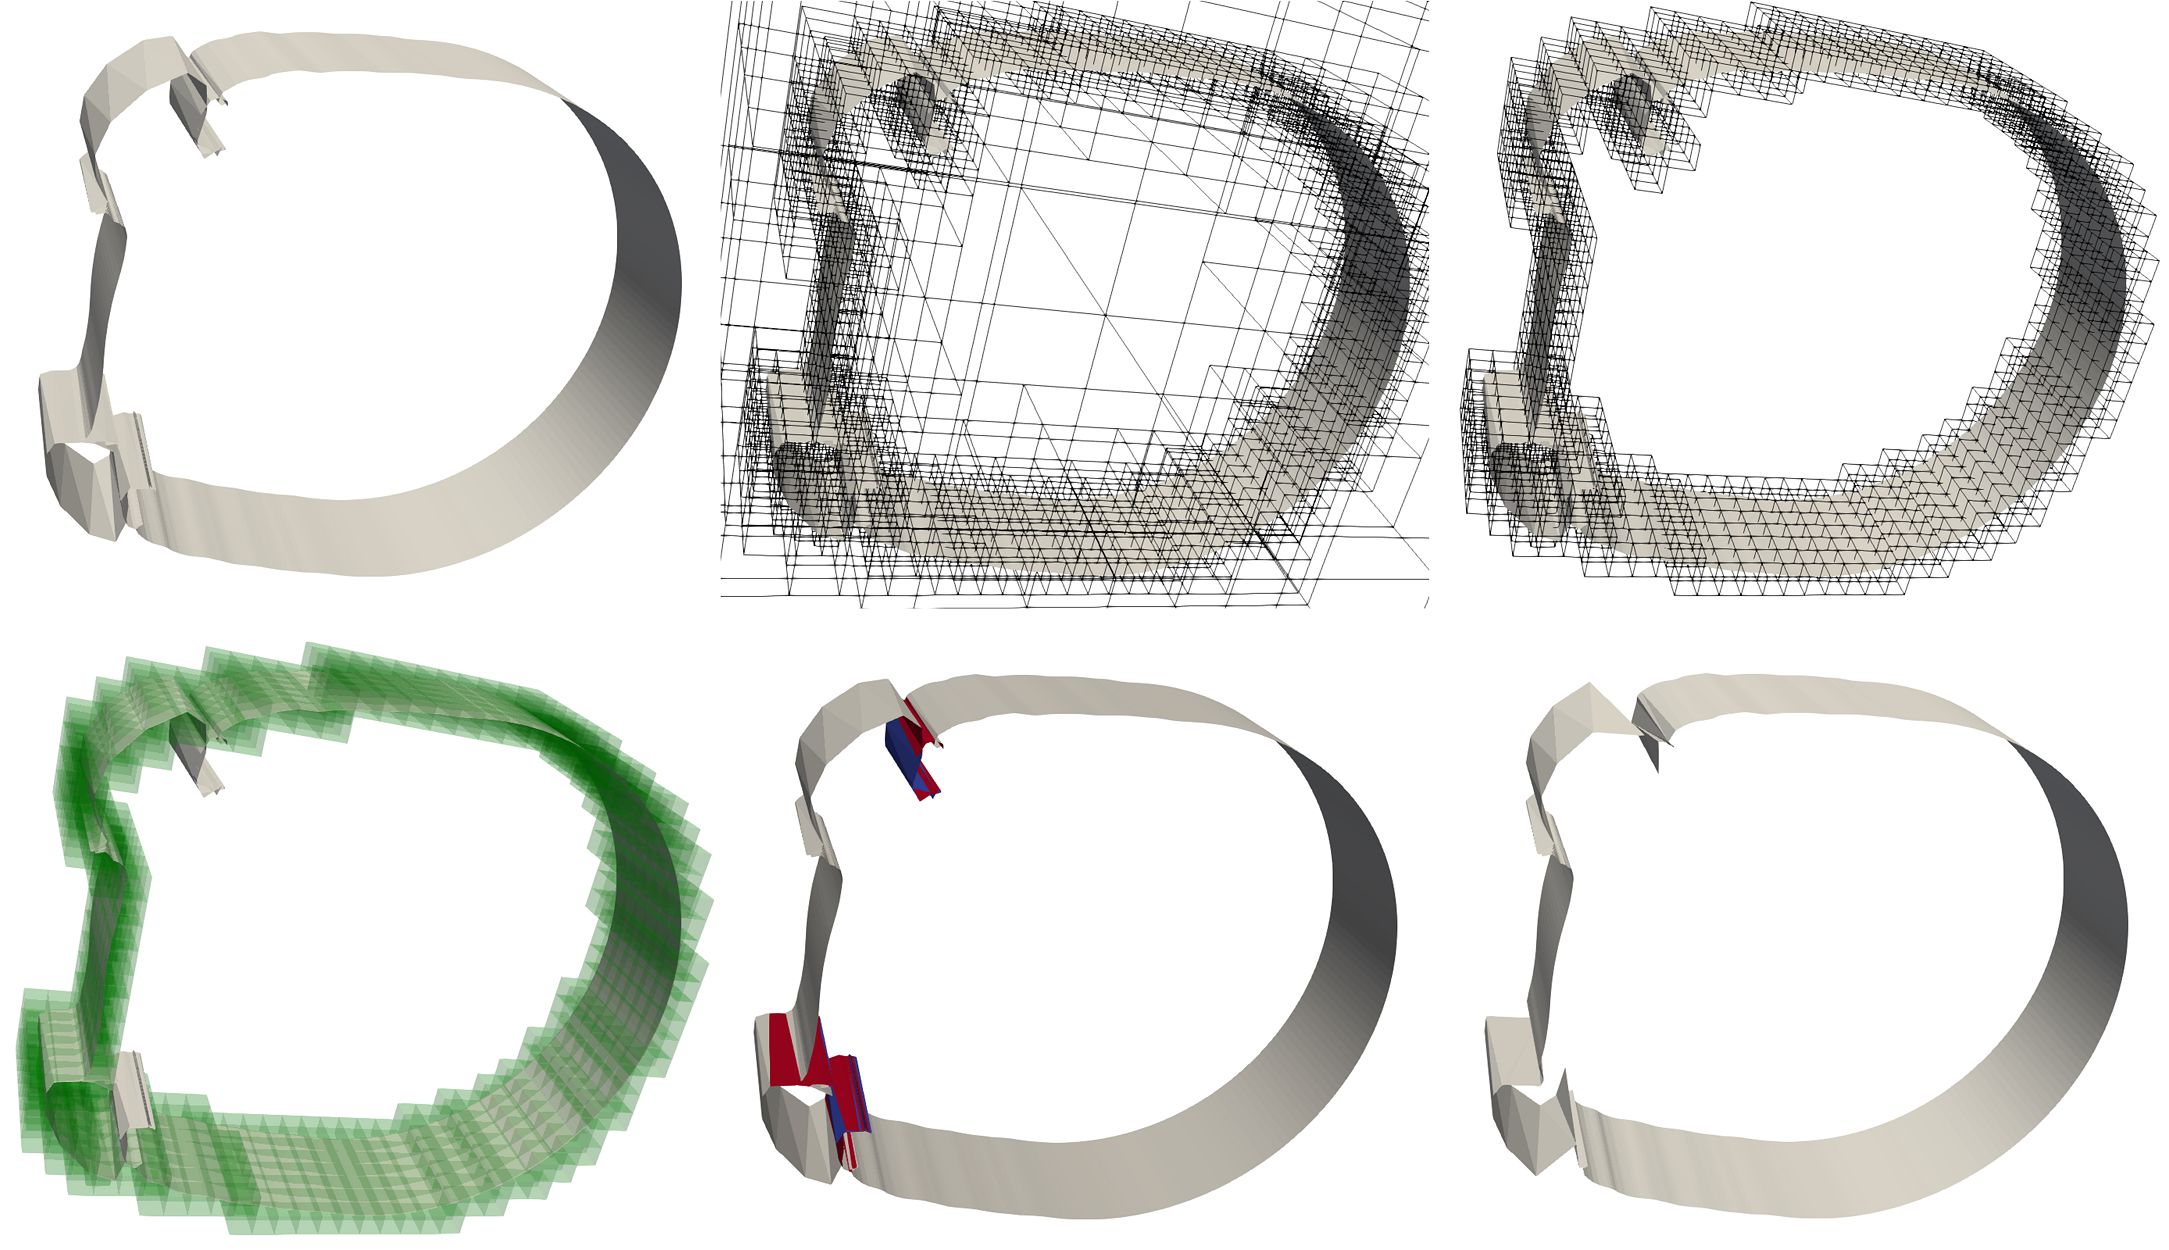
\includegraphics[width=1.0\textwidth]{fig/int_wing_all.png}
\singlespacing
\caption{Устранение самопересечения с использованием подложки поверхностной сетки.}
\label{fig:text_1_int_2}
\end{figure}

Для \textit{псевдотрехмерных профилей} предлагается другой подход к удалению самопересечений (рис.~\ref{fig:text_1_int_2}).
В пространстве строится восьмеричное дерево вложенных кубов, называемое \textit{подложкой}, где корень охватывает всю поверхностную сетку, а дочерние кубы строятся только в случае пересечения с сеткой.
Минимальный размер ячейки подложки выбирается меньше наиболее короткого ребра поверхностной сетки.
Далее определяется внешний слой кроны подложки, и все ячейки, не пересекающие этот слой, помечаются как кандидаты на удаление из сетки.
Также помечаются все ячейки, пересекающие другие ячейки в сетке.
После чего выполняется шаг стягивания сетки по граничным ребрам, входящим в помеченную область.
После этого процесс повторяется итерационно, пока расчетная сетка не будет избавлена от самопересечений.
Такой подход не гарантирует устранение самопересечений на произвольной сетке, однако на псевдотрехмерных профилях он позволяет избавиться от самопересечений без необходимости точного определения точек пересечения пар треугольников.

%----------------------------------

В разделе~3.2 рассматривается проблема сопряжения поверхностной сетки с объемной сеткой и поиска их пересечений для определения поля скоростей вокруг обтекаемого тела.
При расчете ледообразования крайне важным элементом данных является поле скоростей в области, окружающей рассматриваемую поверхность.
Поле скоростей вблизи поверхности влияет на движение жидкой пленки по поверхности, что существенным образом определяет картину обледенения.
Также при использовании модели вторичного увлажнения отскочившие от поверхности капли попадают в свободный поток, и поле скоростей необходимо для расчета траектории их движения и зоны вторичного выпадения.
Так как при перестроении поверхностной сетки построение согласованной объемной сетки является затратной процедурой, то для возможности продолжения расчетов предлагается метод погруженной границы с фиктивными ячейками.

Для реализации метода погруженной границы также используется подложка поверхностной расчетной сетки, и в этом разделе более детально рассматривается вопрос поиска пересечений поверхностной сетки с подложкой.
Для поиска пересечений поверхностной сетки с подложкой используется представление треугольной ячейки $ABC$ с помощью геометрического места точек (ГМТ) $\overline{P}(\beta, \gamma) = \overline{A} + \beta (\overline{B} - \overline{A}) + \gamma (\overline{C} - \overline{A}), \beta \ge 0, \gamma \ge 0, \beta + \gamma \le 1$ и ячейки в форме прямоугольного параллелепипеда в виде ГМТ $x_l \le x_P \le x_h, y_l \le y_P \le y_h, z_l \le z_P \le z_h$ и поиска точек, входящий в оба ГМТ.
Множество точек, входящих в оба указанных ГМТ описывается системой линейных 9 линейных неравенств относительно переменных $\beta$ и $\gamma$, которая решается с помощью метода свертывания, или деформации.

%----------------------------------

В разделе~3.3 рассматривается \textit{метод погруженной границы} с использованием фиктивных ячеек в трехмерной постановке.
В предлагаемом методе строится декартова объемная сетка, в которой ячейки в виде прямоугольных параллелепипедов предварительно разделяются на четыре категории:
COMMON, \textit{внешние ячейки} -- целиком лежащие вне тела (к ним привязаны газодинамические величины, и в них выполняются вычисления), INNER, \textit{внутренние ячейки} -- целиком лежащие внутри тела (к ним не привязаны газодинамические величины, и в них не выполняются вычисления), BORDER, \textit{граничные ячейки} -- все остальные ячейки.
Далее из граничных ячеек выделяются те, для которых меньшая часть объема находится вне тела, а большая -- внутри тела.
Такие ячейки называются \textit{фиктивными}, к ним привязаны газодинамические величины, но они используются только для вычислений, проводимых с соседними COMMON ячейками, (GHOST) (рис.~\ref{fig:text_1_immersed_boundary_method_class} слева).

\begin{figure}[ht]
\centering
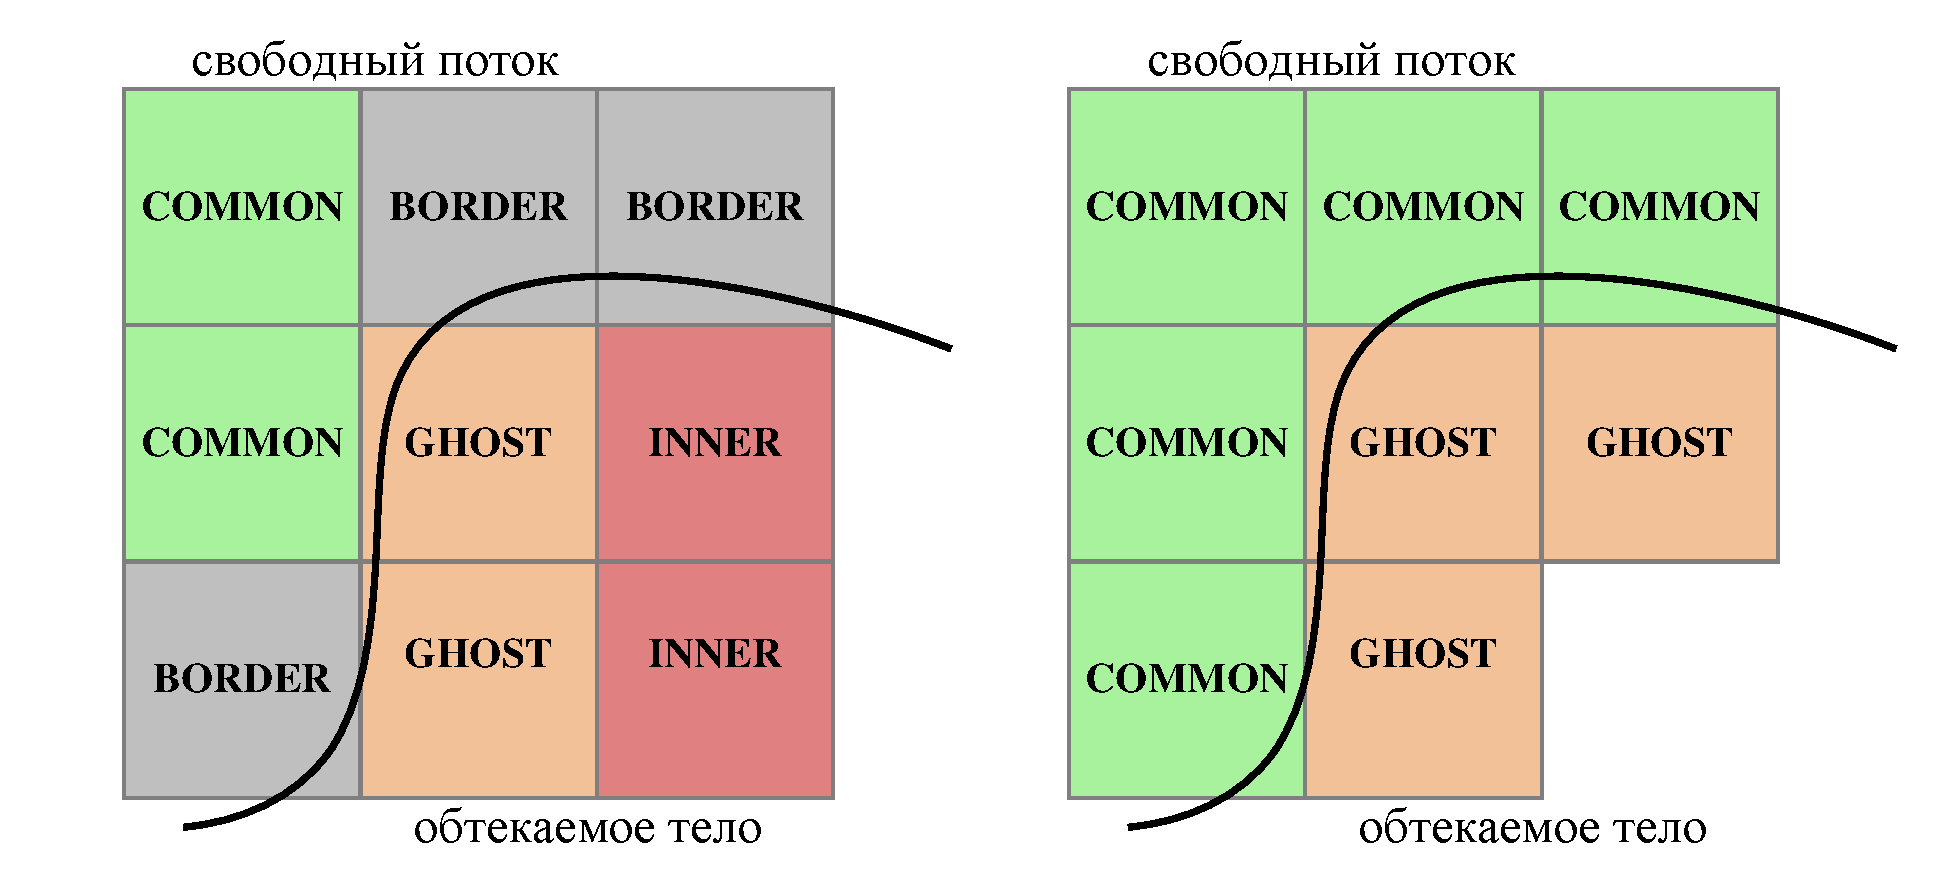
\includegraphics[width=0.8\textwidth]{fig/int_cells_classification_big.pdf}
\singlespacing
\caption{Классификация ячеек.}
\label{fig:text_1_immersed_boundary_method_class}
\end{figure}

После этого выполняется корректировка классификации ячеек для достижения выполнения следующего требования: соседями внутренних ячеек не могут являться ни граничные, ни внешние ячейки.
При этом некоторые внутренние ячейки переходят в класс фиктивных, а все оставшиеся граничные ячейки -- в класс внешних.
После корректировки классификации ячеек на границе внешней области образуется слой фиктивных ячеек. (рис.~\ref{fig:text_1_immersed_boundary_method_class} справа).
На каждой итерации расчетов для фиктивных ячеек требуется выполнить аппроксимацию газодинамических величин (плотность, давление, вектор скорости), чтобы эти фиктивные ячейки могли быть использованы для определения потоков между ними и соседними с ними внешними ячейками.
Аппроксимация скалярных и векторных газодинамических величин в фиктивных ячейкаx выполняется с помощью шаблонов, в которые входят три внешние ячейки, а также точка поверхности, в которой известно направление нормали $\overline{e}_0$.
Наиболее сложной процедурой является определение компонент скорости в фиктивной ячейке $\overline{v}_G$.

В выводах к главе отмечено, что предложенные методы удаления самопересечений поверхностной расчетной сетки, позволяют избежать аварийной остановки расчетов по моделированию ледообразования, продолжение которых невозможно при возникновении этого критического дефекта.
Метод поиска пересечения поверхностной расчетной сетки с подложкой и метод погруженной границы позволяют выполнять расчет поля скоростей без необходимости создания согласованной расчетной сетки в пространстве.

%===================================================================================================

\textbf{Четвертая глава} посвящена задаче разработки методов повышения производительности параллельных вычислений на поверхностных и объемных расчетных сетках в моделях распараллеливания с передачей сообщений и на общей памяти.

%----------------------------------

В разделе~4.1 приводятся показатели распараллеливания в модели с передачей сообщений: \textit{ускорение} $s_{msg}(k) = T_1/T_k$ ($T_i$ -- время выполнения задачи на $i$ процессах), \textit{эффективность} $e_{msg}(k) = s_{msg}(k)/k$.
Для распараллеливания вычислений область задачи нужно разбить на подобласти (совокупности расчетных ячеек, \textit{домены}, \textit{партиции}), распределить домены между процессами и организовать обмен сообщениями между доменами.
Эта задача эквивалентна задаче декомпозиции \textit{дуального графа} расчетной сетки $G = (V, E)$ (вершины графа соответствуют ячейкам сетки, ребро графа связывает две вершины, соответствующие соседним ячейкам), для которой рассматриваются показатели качества декомпозиции.
\textit{Неравномерность декомпозиции} $D = \max_{0 \le i < k}{ \left( n_i - \frac{n}{k} \right) }$, $D^{*} = \frac{D}{n/k}$ ($n = |V|$, $n_i$ -- количество вершин в $i$-ом домене) характеризует простаивание вычислительных ресурсов во время обработки наибольшего домена.
\textit{Наибольшая длина границы между парой доменов} $L_{ij} = \left| \{ e \in E: \{ d(e_a), d(e_b) \} = \{ i, j \} \} \right|$, $L = \max_{0 \le i < j < k}{L_{ij}}$ ($e_a$, $e_b$ -- инцидентные ребру $e$ вершины, $d(v)$ -- домен вершины $v$) определяет длительность информационных обменов между доменами.
\textit{Суммарная длина границ между доменами} $I = \sum_{0 \le i < j < k}{L_{ij}}$ определяет общий объем данных при обмене сообщениями.

%----------------------------------

В разделе~4.2 рассматривается проблема распределения вычислительной нагрузки между партициями при проведении вычислений на блочно-структу\-рированной расчетной сетке.
При распределении каждый блок целиком попадает в какую-либо партицию.
Описывается архитектура блочно-структуриро\-ванной расчетной сетки с поддержкой дробления блоков, применение которого позволяет уменьшить значение показателя $D$ неравномерности распределения.

Рассматривается задача распределения $m$ блоков расчетной сетки между $k$ партициями в следующем виде.
Пусть $X$ -- множество чисел $x_i > 0$, $i \in M$, $M = [0, m - 1]$.
Разбиение множества $X$ на подмножества $K = [0, k - 1]$ -- это отображение $\gamma: M \rightarrow K$.
Веса результирующих подмножеств определяются как $X_j = \sum_{i \in M, \ \gamma(i) = j}{x_i}$.
Требуется найти разбиение, минимизирующее наиболее тяжелое подмножество $X^{max} = \max_{j \in K}{X_j}$.

Поставленная задача о разделении множества $m$ весов на $k$ подмножеств при условии минимизации $X^{max}$ связана с большими вычислительными затратами.
Существует алгоритм решения этой задачи, основанный на решении другой, так называемой $z$-задачи, которая формулируется следующим образом: определить, существует ли такое разбиение множества $m$ весов на $k$ подмножеств, для которого выполнено условие $X^{max} \le z$.
Используя $z$-задачу, исходную задачу о разбиении с минимизацией $X^{max}$ можно решить с помощью бинарного поиска.
Решение же $z$-задачи выполняется методом ветвей и границ с односторонним обходом дерева вариантов разбиения.
Такой подход хоть существенно сокращает время работы алгоритма, однако не снижает его сложность и при больших значениях $m$ и $k$ неприменим.

Рассматривается жадный алгоритм поиска приближенного решения задачи разделения множества $m$ весов на $k$ подмножеств.
В этом алгоритме последовательно обрабатываются все веса, начиная с наибольшего.
Каждый необработанный вес добавляется к наиболее легкому на текущий момент подмножеству.
Жадный алгоритм имеет сложность $O(m(\log m + \log k) + k)$ при использовании упорядоченного множества для хранения текущих весов подмножеств, а его эффективность оценивается с помощью следующей леммы.

\textbf{Лемма}. \textit{Для жадного алгоритма распределения весов $X$ между подмножествами $K$ верна оценка $X^{max} - X^{avg} \le \max_{i \in M}{r_i}$, где $X^{avg} = \frac{1}{k}\sum_{j \in K}{X_j}$, $r_i = \max{( x_i - \frac{1}{k} \sum_{p = i}^{m}{x_p}, 0)}$.}

Характеристика $X^{max} - X^{avg}$ соответствует показателю $D$.
Из леммы делается вывод о деградации показателя $D$ при наличии крупных блоков.
Для снижения значения $D$ предлагаются алгоритмы распределения с использованием дробления блоков.

Рассматривается механизм дробления трехмерного блока размера $a \times b \times c$, заключающийся в разрезании его на два блока по одному из измерений.
Для построения алгоритма распределения блоков по партициям с минимизацией параметра $D$ рассматривается задача о выделении из блока размера $a \times b \times c$ части заданного размера $t \ge 0$.
Минимальное количество разрезов, требуемое для решения этой задачи, обозначается $P_{a \times b \times c}^t$ и вычисляется как
\begin{equation}\label{eqn:par_pnmkt_3d}
P_{a \times b \times c}^t =
	\begin{cases}
		+\infty, & \text{если } t > abc \\
		0, & 
			\begin{aligned}
				\text{если } & (t = 0) \\[-4pt]
				& \vee (t = abc)
			\end{aligned} \\
		P_{b \times c}^t, & \text{если } a = 1 \\
		P_{a \times c}^t, & \text{если } b = 1 \\
		P_{a \times b}^t, & \text{если } c = 1 \\
		\begin{aligned}
			\min\big[
				& \min_{\substack{1 \le a_1 < a \\ 0 \le t_1 < t}}{\{P_{a_1 \times b \times c}^{t_1} + P_{(a - a_1) \times b \times c}^{t - t_1}\}}, \\[-2pt]
				& \min_{\substack{1 \le b_1 < b \\ 0 \le t_1 < t}}{\{P_{a \times b_1 \times c}^{t_1} + P_{a \times (b - b_1) \times c}^{t - t_1}\}}, \\[-2pt]
				& \min_{\substack{1 \le c_1 < c \\ 0 \le t_1 < t}}{\{P_{a \times b \times c_1}^{t_1} + P_{a \times b \times (c - c_1)}^{t - t_1}\}}
			\big] + 1
		\end{aligned}, & 
			\begin{aligned}
				\text{если } & (\min(a, b, c) > 1) \\[-4pt]
				& \wedge (0 < t < abc)
			\end{aligned}
	\end{cases}
\end{equation}
где $P_{a \times b}^t$ для двумерного случая вычисляется аналогично, а $P_a^t$ принимает значение $+\infty$ при $t > a$, значение $0$ при $t \in \{0, a\}$, и значение $1$ при $0 < t < a$.
Доказываются основные свойства значений $P_{a \times b \times c}^t$, среди которых симметричность по размерам блока, симметричность по размеру выделяемой части $P_{a \times b \times c}^t = P_{a \times b \times c}^{abc - t}$ и ограниченность $P_{a \times b \times c}^t \le 5$.
Оценивается сложность вычисления значений $P_{a \times b \times c}^t$ для всех $b \le a$, $c \le a$, составляющая $\frac{1}{96}a^6 + o(a^6)$.
С учетом приведенных свойств справедлива лемма о минимальном количестве разрезов в алгоритме точного распределения блоков по партициям.

\textbf{Лемма}. \textit{При распределении произвольного количества блоков расчетной сетки с суммарным количеством ячеек $n$ по $k$ партициям и выполнении условия $k \mid n$ равномерное распределение с показателем $D = 0$ может быть достигнуто с использовнием не более $5(k - 1)$ разрезов блоков.}

Так как точное распределение связано с большим количеством разрезов блоков и с высокими затратами на вычисление значений $P_{a \times b \times c}^t$, а также с возможным образованием слишком мелких блоков, то рассматриваются приближенные алгоритмы распределения блоков по партициям с использованием дроблений.
Для описания алгоритмов используются обозначения: $B$ -- множество блоков, $b$ -- блок, $P$ -- множество партиций, $p$ -- партиция.
Партиция $p$ содержит множество блоков $p.B$.
Для блока, множества блоков и партиции определено понятие веса $w$, выраженного в количестве ячеек.
Дробление блока по наиболее протяженному измерению в позиции $i$ обозначается $\{b_1, b_2\} = b.cut(i)$.

Первый рассматриваемый алгоритм основан на жадном распределении.
Дано множество блоков $B$.
Сначала выполняется их распределение с помощью жадного алгоритма.
Если после этого требуемое значение параметра $D^{*} \le \epsilon$ не достигнуто, то выполняется дробление наибольшего блока пополам по наиболее протяженному измерению, после чего жадный алгоритм применяется повторно.
Алгоритм имеет сложность $O(m \log m + \sigma(m \log k + k + \sigma))$, где $\sigma \ge 1$ -- количество разрезов блоков, и гарантированно завершает работу при $\epsilon \ge \frac{\lceil \mu \rceil - \mu}{\mu}$, где $\mu = \frac{B.w}{k}$. 
Последовательность дроблений блоков сетки для достижения заданного значения показателя $D^{*}$ при распределении между $k$ партициями будем называть \textit{подготовкой сетки}.
Для демонстрации важности сокращения количества дроблений блоков приводятся результаты эксперимента по выполнению расчетов на блочно-структурированной расчетной сетке, с подготовкой для разных значений $k$ и $D^{*}$ при помощи дробления наибольшего блока.

\begin{figure}[ht]
\centering
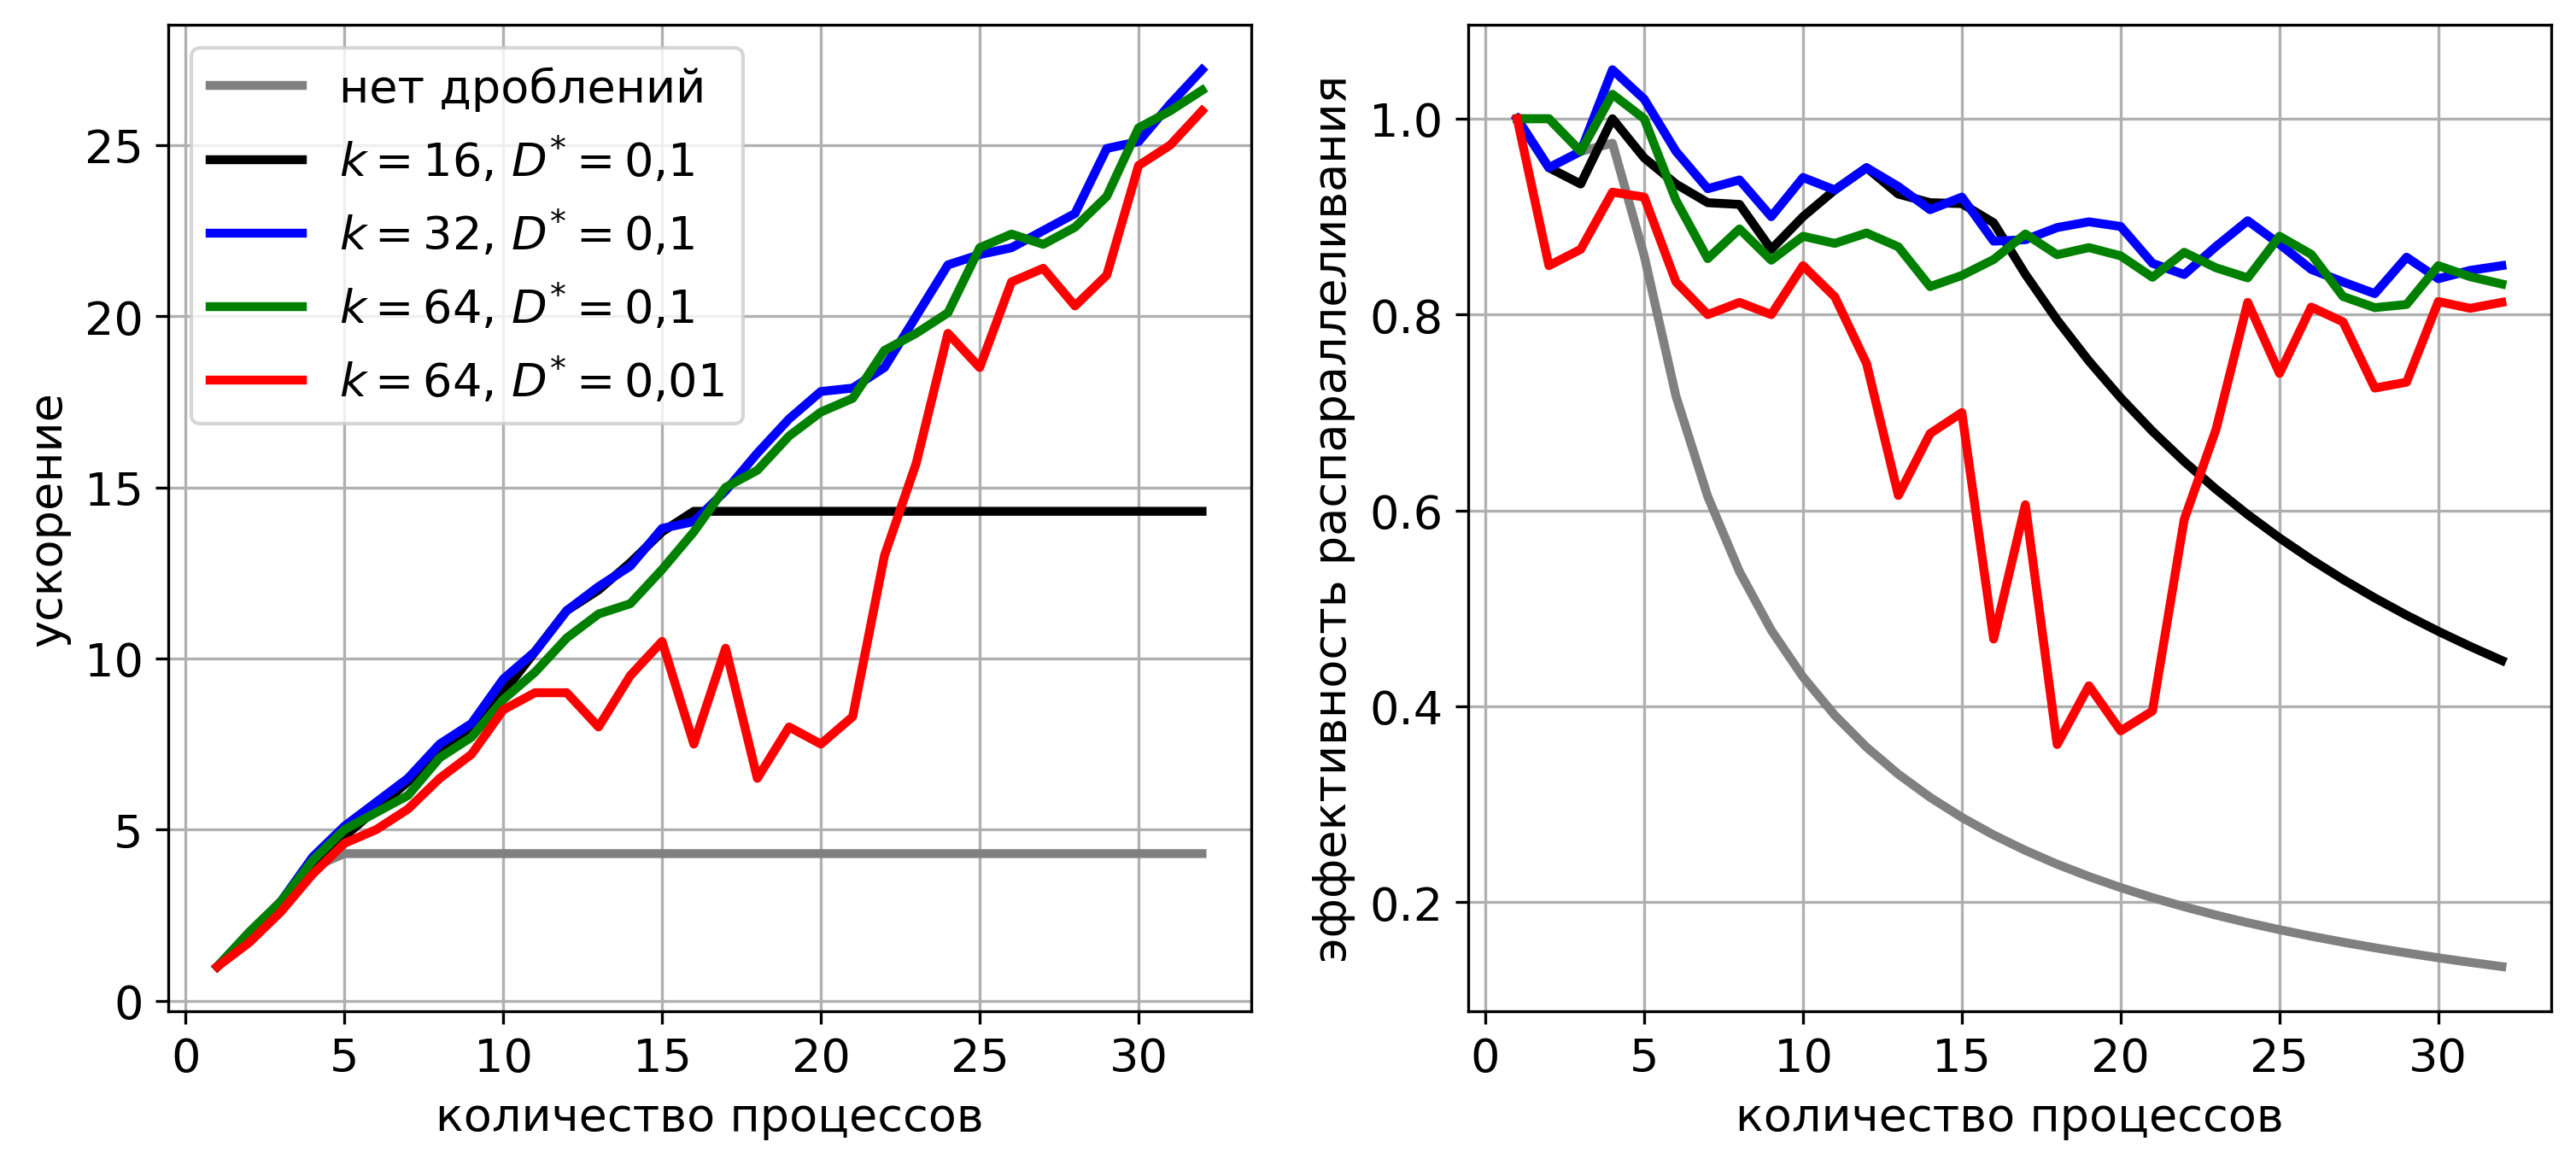
\includegraphics[width=1.0\textwidth]{./fig/par_scaling_with_prepare_big.png}
\singlespacing
\caption{Масштабирование вычислений с подготовкой сетки.}
\label{fig:par_scaling_with_prepare}
\end{figure}

На рис.~\ref{fig:par_scaling_with_prepare} представлены результаты численных экспериментов масштабирования вычислений на блочно-структурированной расчетной сетке на 1-32 процессах.
На неподготовленной сетке ("нет дроблений") и при подготовке для $k = 16$ наблюдается ограничение ускорения, обусловленное наличием крупных блоков. 
При подготовке сетки для $k = 32$ и $k = 64$ с допустимым отклонением $D^{*} = 0{,}1$ наблюдается примерно одинаковое ускорение и эффективность распараллеливания с ростом количества процессов.
Это говорит о том, что подготовка сетки для большего количества процессов, чем реально будет использоваться для запусков, избыточно.
При подготовке сетки для $k = 64$ и $D^{*} = 0{,}01$ наблюдается деградация эффективности распараллеливания из-за возрастания количества дроблений, что приводит к увеличению объема межпроцессных обменов.
Так как подготовка расчетной сетки с помощью дробления наиболее крупных блоков при снижении требуемого значения $D^{*}$ приводит к сильному увеличению количества разрезом и деградации производительности, то предлагается подход к уменьшению количества разрезов.

Будем считать, что размеры блока $b$ отсортированы по убыванию, сторона по первому измерению $b.a$ является наибольшей, и разрезы будем выполнять только этому измерению.
Для запрета появления слишком тонких блоков будем запрещать выполнять разрезы блока слишком близко к границе (деление блока будем выполнять только в сегменте $[\delta, b.a - \delta]$).
Также будем запрещять появление блоков с весом меньше $\Delta$.
Позицию разреза $i$ блока $b$ будем называть \textit{допустимой}, если $i \in [\delta, b.a - \delta]$ и $\min(i, b.a - i)\frac{b.w}{b.a} \ge \Delta$ (то есть разрез выполнен вдали от границы блока и не порождает мелкие блоки).

Для реализации алгоритма с уменьшением количества дроблений блоков рассмотрим четыре основные операции.
\texttt{FillFullUnder}: для заданного множества блоков $B$ и множества партиций $P$ найти такой блок $b \in B$ и партицию $p \in P$, что величина $p.w + b.w$ является максимально возможной, но не превышающей заданное значение $\tau$.
\texttt{FillPartUnder}: для $B$ и $P$ найти $b \in B$ и $p \in P$, а также допустимую позицию разреза $i$, что величина $p.w + b.w \frac{i}{b.a}$ является максимально возможной, но не превышающей заданное значение $\tau$.
\texttt{FillFullAbove}: для $B$ и $P$ найти $b \in B$ и $p \in P$, что величина $p.w + b.w$ является минимально возможной превышающей заданное значение $\tau$.
\texttt{FillPartAbove}: для $B$ и $P$ найти $b \in B$ и $p \in P$, а также допустимую позицию разреза $i$, что величина $p.w + b.w \frac{i}{b.a}$ является минимально возможной превышающей заданное значение $\tau$.
Алгоритм распределения множества блоков по партициям будем определять как последовательность попыток произвести одну из введенных четырех операций, пока множество распределяемых блоков не станет пустым $B$.
При этом параметр $\tau$ имеет смысл максимально допустимого размера партиции на текущий момент.

\textbf{Алгоритм}. \textit{Параметрический алгоритм $\mathscr{A}_{U/u}^{A/a}$ распределения множества блоков по партициям с уменьшением количества дроблений.}
\begin{algorithm}
\DontPrintSemicolon
\SetKw{Continue}{continue}
\KwInput{$B$ -- множество блоков, $k$ -- количество партиций, $\delta$ -- ограничение на позицию разреза, $\Delta$ -- минимальный размер блока, $U$ -- использование \texttt{FillFullUnder}, $u$ -- использование \texttt{FillPartUnder}, $A$ -- использование \texttt{FillFullAbove}, $a$ -- использование \texttt{FillPartAbove}.}
\KwOutput{$P$ -- множество результирующих партиций.}
\Fn{\texttt{DistributeMinCuts<}$U$, $u$, $A$, $a$\texttt{>}($B$, $k$, $\delta$, $\Delta$)}
{
	$P \leftarrow \{ p : p.B = \emptyset, \forall i \in [0, k - 1] \}$\;
	$\tau \leftarrow \frac{B.w}{k}$\;
	\While{$B \ne \emptyset$}
	{
		\If{$U \wedge (((b, p) \leftarrow FillFullUnder(B, P, \tau)) \ne null)$}
		{
			$(B, p.B) \leftarrow (B \setminus \{b\}, p.B \cup \{b\})$\;
			\Continue\;
		}
		\If{$u \wedge (((b, p, i) \leftarrow FillPartUnder(B, P, \tau, \delta, \Delta)) \ne null)$}
		{
			$\{ b_1, b_2 \} \leftarrow b.cut(i)$\;
			$(B, p.B) \leftarrow ((B \setminus \{ b \}) \cup \{ b_2 \}, p.B \cup \{ b_1 \})$\;
			\Continue\;
		}
		\If{$a \wedge (((b, p, i) \leftarrow FillPartAbove(B, P, \tau, \delta, \Delta)) \ne null)$}
		{
			$\{ b_1, b_2 \} \leftarrow b.cut(i)$\;
			$(B, p.B) \leftarrow ((B \setminus \{ b \}) \cup \{ b_2 \}, p.B \cup \{ b_1 \})$\;
			$\tau \leftarrow p.w$\;
			\Continue\;
		}
		\If{$A \wedge (((b, p) \leftarrow FillFullAbove(B, P, \tau)) \ne null)$}
		{
			$(B, p.B) \leftarrow (B \setminus \{b\}, p.B \cup \{b\})$\;
			$\tau \leftarrow p.w$\;
			\Continue\;
		}
	}
	\KwRet $P$\;
}
\end{algorithm}

Каждая из операций заполнения при реализации множества блоков и множества партиций с помощью упорядоченных по весу множеств имеет сложность $O(m + k)$ в среднем и $O(mn)$ в худшем случае, сложность алгоритма в среднем равна $O((m + \sigma)(m + k))$, где $\sigma$ -- количество выполненных в результате разрезов.
Порядок применения операций продиктован стремлением сдержать значение $\tau$ и уменьшить количество дроблений.
Параметрический алгоритм $\mathscr{A}_{U/u}^{A/a}$ представляет собой группу из 16 алгоритмов, однако для применения дроблений и гарантированного завершения работы необходимо выполнение условия $U \wedge A \wedge (u \vee a)$, что приводит к группе из трех алгоритмов $\mathscr{A}_{1/0}^{1/1}$, $\mathscr{A}_{1/1}^{1/0}$, $\mathscr{A}_{1/1}^{1/1}$.

\begin{figure}[ht]
\centering
\begin{tabular}{l}
\begin{subfigure}{1.0\textwidth}\centering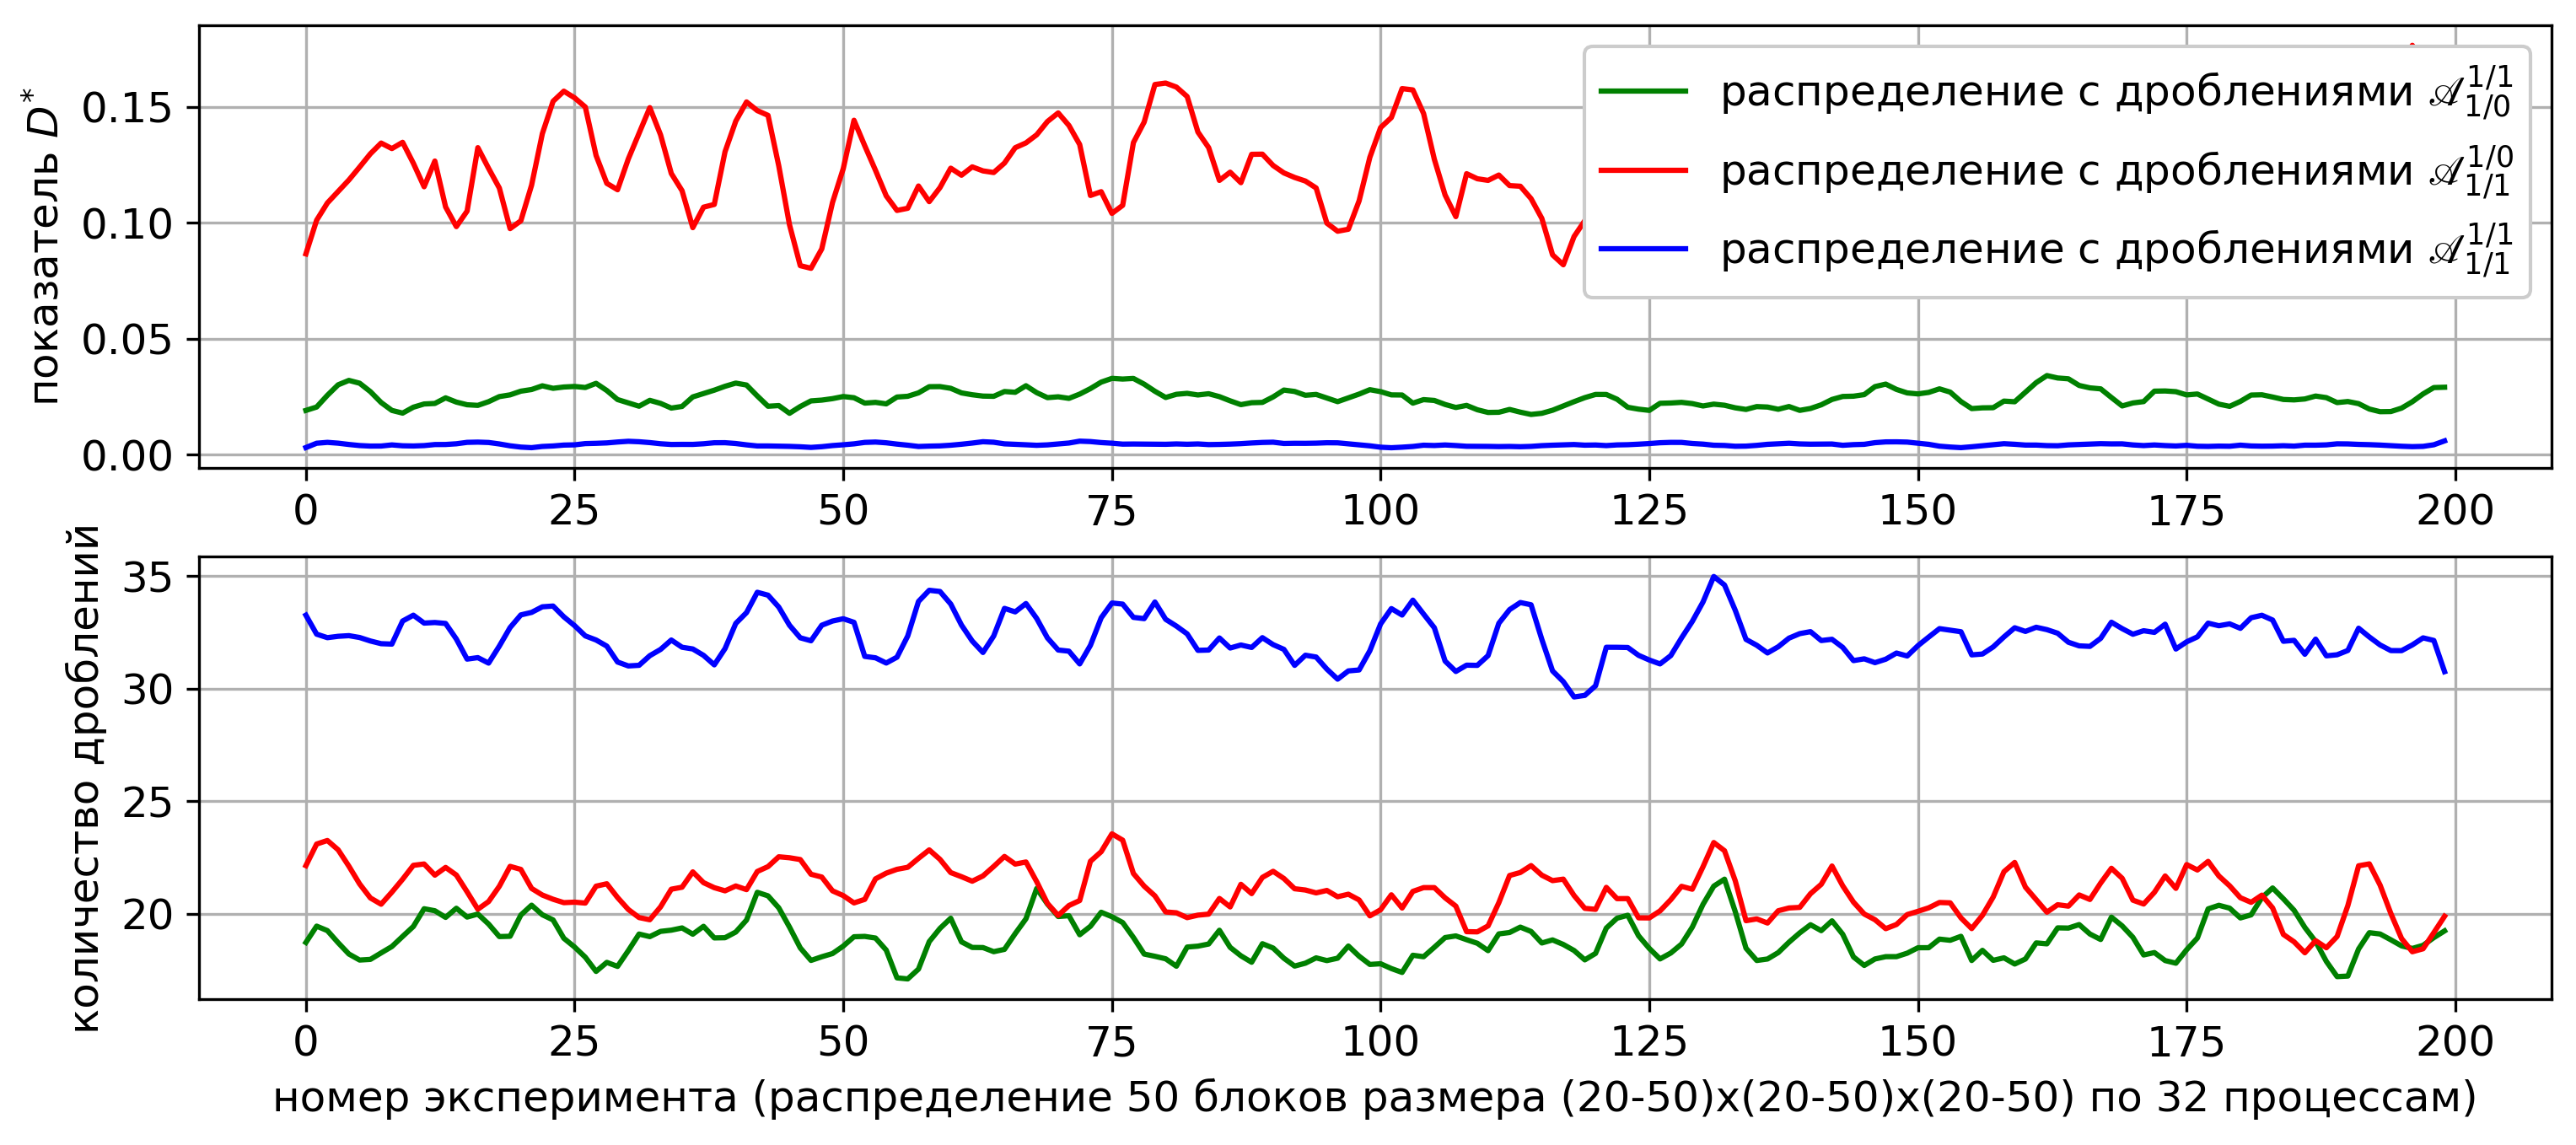
\includegraphics[width=1.0\columnwidth]{fig/par_chart_distr_50_20_50_32.png}\caption{Результаты распределения 50 блоков по 32 партициям.}\end{subfigure} \\
\begin{subfigure}{1.0\textwidth}\centering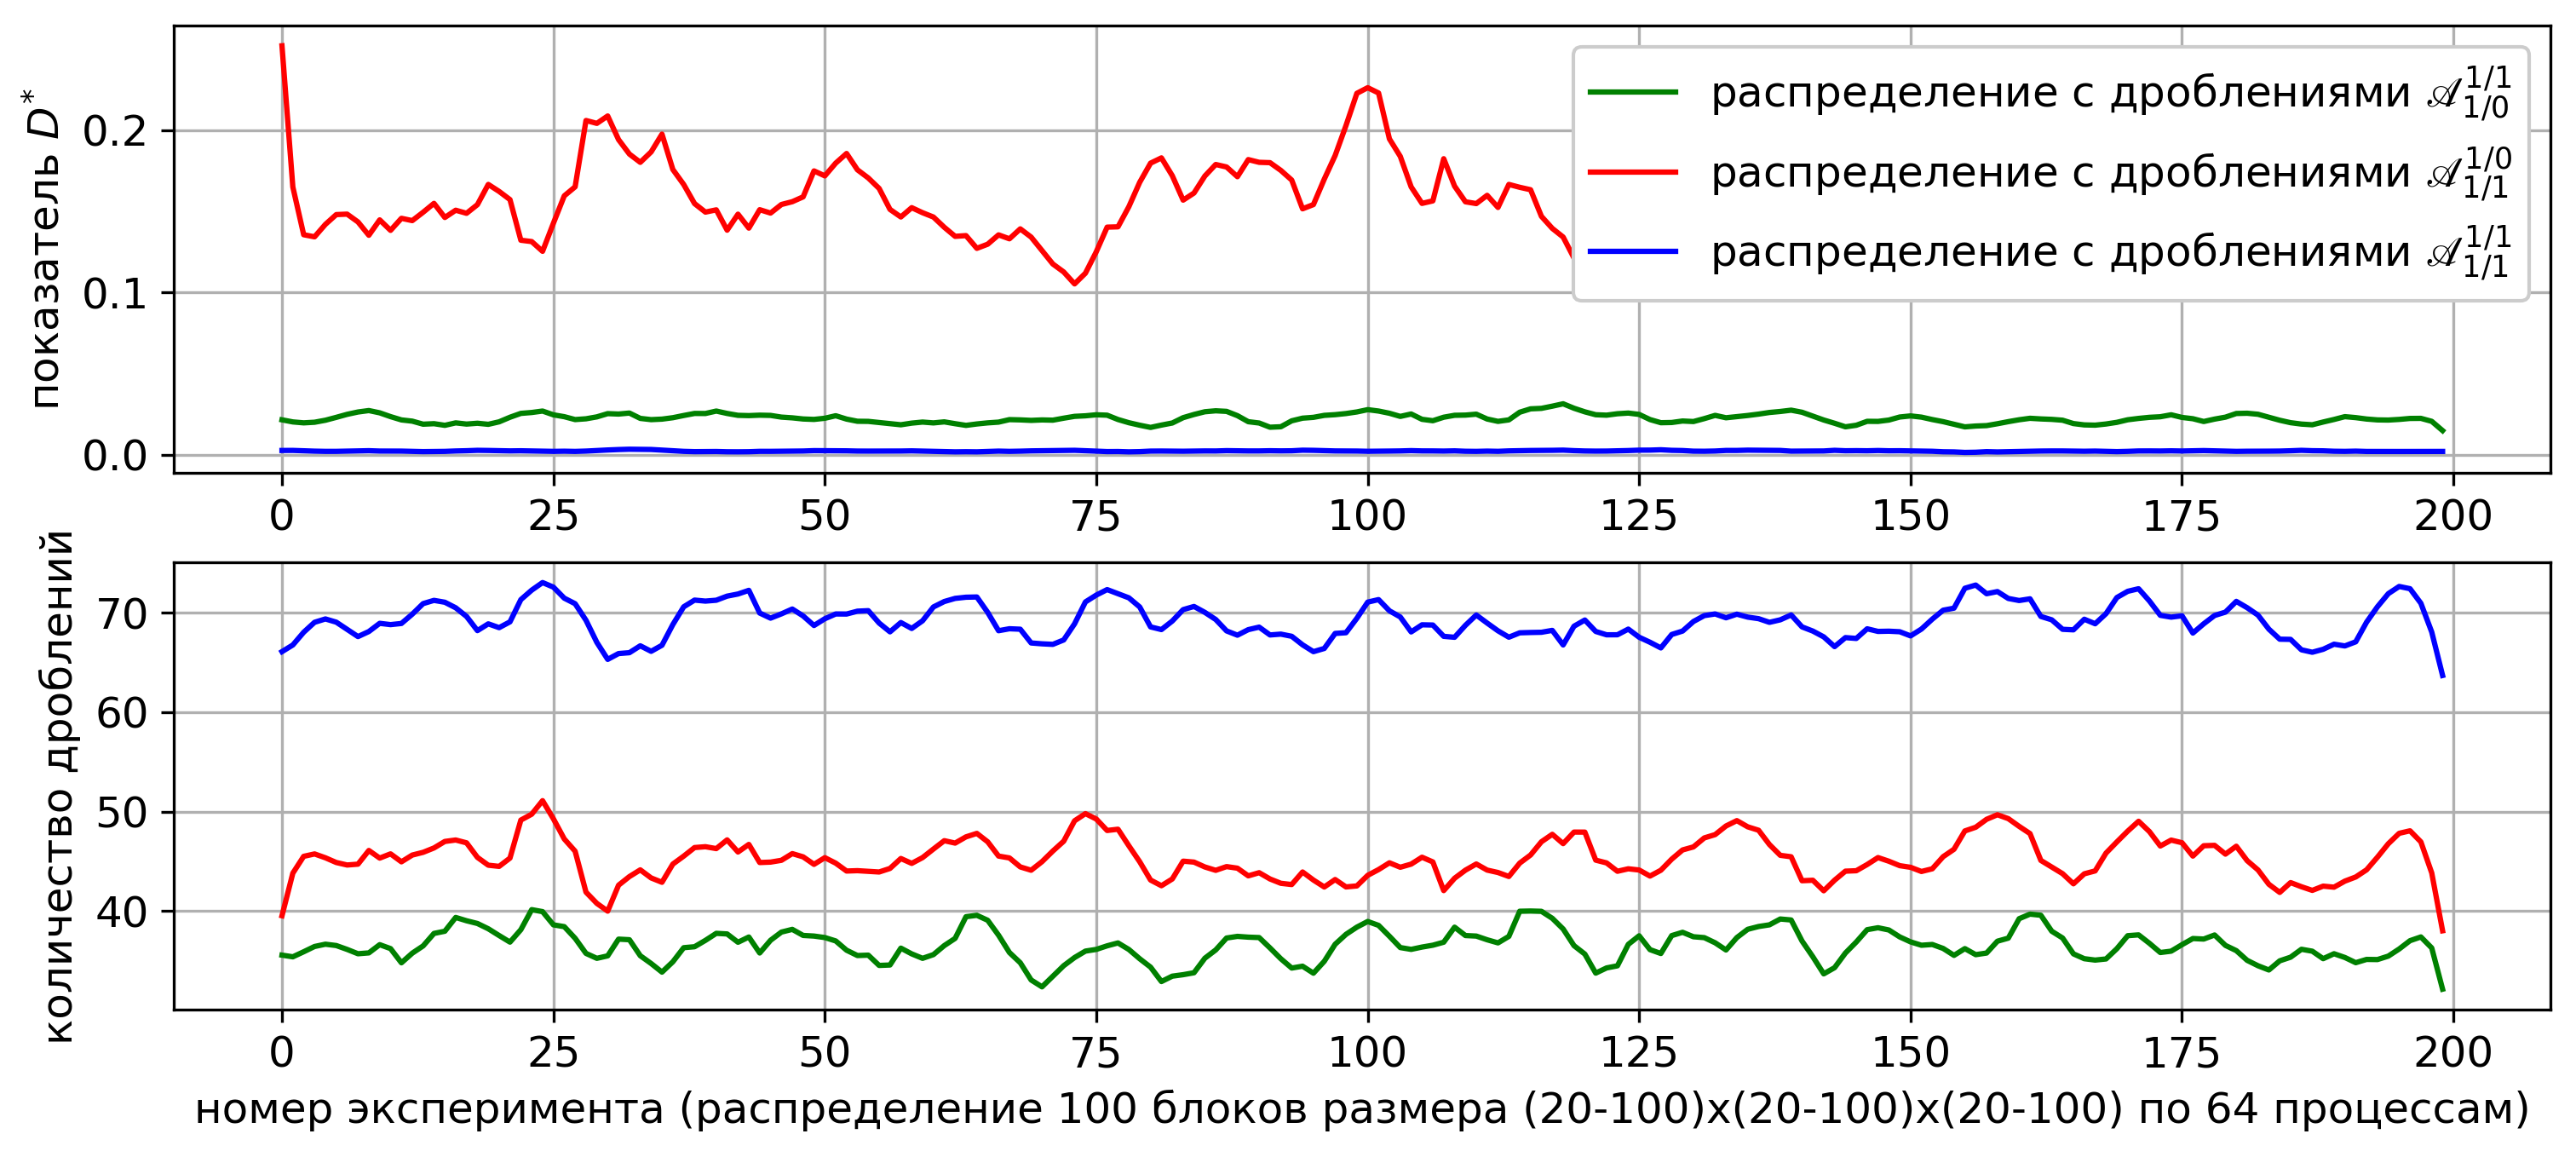
\includegraphics[width=1.0\columnwidth]{fig/par_chart_distr_100_20_100_64.png}\caption{Результаты распределения 100 блоков по 64 партициям.}\end{subfigure}
\end{tabular}
\singlespacing
\caption{Графики $D^{*}$ и $\sigma$ при использовании алгоритмов $\mathscr{A}_{1/0}^{1/1}$, $\mathscr{A}_{1/1}^{1/0}$, $\mathscr{A}_{1/1}^{1/1}$.}
\label{fig:min_cuts_distr}
\end{figure}

Результаты работы алгоритмов $\mathscr{A}_{1/0}^{1/1}$, $\mathscr{A}_{1/1}^{1/0}$, $\mathscr{A}_{1/1}^{1/1}$ сравнивались между собой по двум характеристикам: показателю неравномерности рааспределения $D^{*}$ и количеству разрезов $\sigma$ (рис.~\ref{fig:min_cuts_distr}).
Алгоритм $\mathscr{A}_{1/1}^{1/1}$ порождает наиболее равномерное распределение и приводит к наибольшему количеству дроблений, так как онн использует обе операции заполнения частями блоков (и снизу, и сверху).
Алгоритм $\mathscr{A}_{1/1}^{1/0}$ порождает наименее равномерное распределение, так как для заполнения сверху он использует только целые блоки, что приводит к росту ограничения $\tau$ в процессе работы алгоритма.
Алгоритм $\mathscr{A}_{1/0}^{1/1}$ является наиболее предпочтительным среди трех рассмотренных алгоритмов, так как по равномерности распределения он не сильно уступает алгоритму $\mathscr{A}_{1/1}^{1/1}$, а по количеству разрезов явялется наилучшим.

%----------------------------------

В разделе~4.3 рассматривается декомпозиция поверхностной неструктурированной расчетной сетки и предлагается алгоритм сглаживания границ между доменами.
Отмечены два используемых метода декомпозиции, отличающиеся показателями $D$ и $L$.
Метод декомпозиции с помощью \textit{наращивания доменов} с использованием генетического алгоритма для корректировки положения инициирующих вершин порождает неравномерное распределение вершин по доменам с достаточно гладкими границами.
Метод \textit{иерархического деления пополам} по наиболее протяженному геометрическому направлению наоборот порождает равномерное распределение вершин по доменам с протяженными <<пилообразными>> границами.

Алгоритм сглаживания границы между доменами рассматривается на неструктурированной поверхностной расчетной сетке, применяется к паре доменов и направлен на уменьшение длины границы между ними с сохранением баланса количества ячеек в этих доменах.
Алгоритм рассматривается для границы в виде простой цепи ребер сетки.
Сначала в цепи ищутся все пригодные для сглаживания границы \textit{шаблоны} -- локальные преобразования, уменьшающие длину границы.
После нахожения потенциально пригодных шаблонов выполняется разметка влияния шаблонов друг на друга, шаблон может повлиять только на своих непосредственных соседей.
Последним шагом алгоритма является выбор подмножества независимых шаблонов, которые могут быть применены одновременно и не нарушают суммарного баланса ячеек между доменами.
Ввиду того, что применение каждого шаблона уменьшает длину границы на 1, задача поиска оптимального решения может быть сформулирована в виде поиска в множестве шаблонов подмножества максимального размера, не содержащего конфликтующих шаблонов.
Задачу можно сформулировать в терминах динамического программирования.
Для этого рассматривается функция $B(t, u, x)$, отражающая изменение длины границы при решении задачи на множестве шаблонов $\{ t' \in T : t' \ge t \}$ при условии изменения баланса ячеек на $u$ единиц.
Параметр $x$ является булевым и принимает значение $1$, если шаблон $t$ вошел в решение, и $0$ -- в противном случае.
Решением поставленной задачи является значение $\min_{x \in \{0, 1\}}{B(t_0, 0, x)}$, где $t_0$ -- первый шаблон на рассматриваемой цепи.

Решение задачи начинается с последнего шаблона $t_n$, для которого все множество используемых шаблонов состоит только из него самого, и
\begin{equation*}
	\left\{
		\begin{aligned}
			& B(t_n, 0, 0) = 0 \\
			& B(t_n, U(t_n), 1) = -1
		\end{aligned}
	\right.
\end{equation*}
для всех остальных значений $u$ значение функции $B(t_n, u, x)$ не определено, будем считать его равным $+\infty$ (это означает, что на последнем шаблоне кроме значений $0$ и $U(t_n)$ недостижимы другие значения изменения количества ячеек в домене $U$).

Пусть задача решена для некоторого шаблона $t_{k + 1}$.
Рассмотрим переход к решению для шаблона $t_k$.
Сначала все значения $B(t_k, u, x)$ принимаются равными $+\infty$.
Во-первых, имея любое допустимое решение для шаблона $t_{k + 1}$ мы можем получить решение для шаблона $t_k$, просто проигнорировав этот шаблон, то есть для всех $u$, для которых найдено решение для шаблона $t_{k + 1}$, выполним следующую операцию:
\begin{equation*}
	B(t_k, u, 0) = \min \left( B(t_{k + 1}, u, 0), B(t_{k + 1}, u, 1) \right)
\end{equation*}

Второй момент связан с попыткой использования шаблона $t_k$.
Если $t_k \cap t_{k + 1} = \emptyset$, то есть конфликта нет, то шаблон $t_k$ можно использовать вне зависимости от того, был ли использован шаблон $t_{k + 1}$.
То есть для всех $u$, для которых было найдено решение для шаблона $t_{k + 1}$ выполним следующее действие:
\begin{equation*}
	B(t_k, u + U(t_k), 1) = B(t_k, u, 0) - 1
\end{equation*}

И наконец в случае конфликтующих $t_k$ и $t_{k + 1}$ мы можем использовать шаблон $t_k$ только в том случае, если не был использован шаблон $t_{k + 1}$, то есть для всех $u$ для которых $B(t_{k + 1}, u, 0) \ne +\infty$ нужно выполнить операцию
\begin{equation*}
	B(t_k, u + U(t_k), 1) = B(t_{k + 1}, u, 0) - 1
\end{equation*}

Алгоритм выбора в множестве шаблонов максимального подмножества без конфликтов имеет сложность $O \left( |T| \cdot (U^{max} - U^{min} + 1) \right)$, где $U^{min} = \frac{1}{2} \sum_{t \in T}{(U(t) - |U(t)|)}$ и $U^{max} = \frac{1}{2} \sum_{t \in T}{(U(t) + |U(t)|)}$ -- нижняя и верхняя границы баланса ячеек, $U(t)$ -- изменение баланса ячеек при использовании шаблона $t$.

Использование алгоритма сглаживания границ между доменами позволяет находить точное решение для фиксированного множества рассматриваемых шаблонов и выбранной пары доменов.
Применение алгоритма приводит к сокращению длин границ между доменами примерно на 10\%.
Сложность алгортма сглаживания границ позволяет использовать его для промышленных расчетов.

\begin{figure}[!ht]
\centering
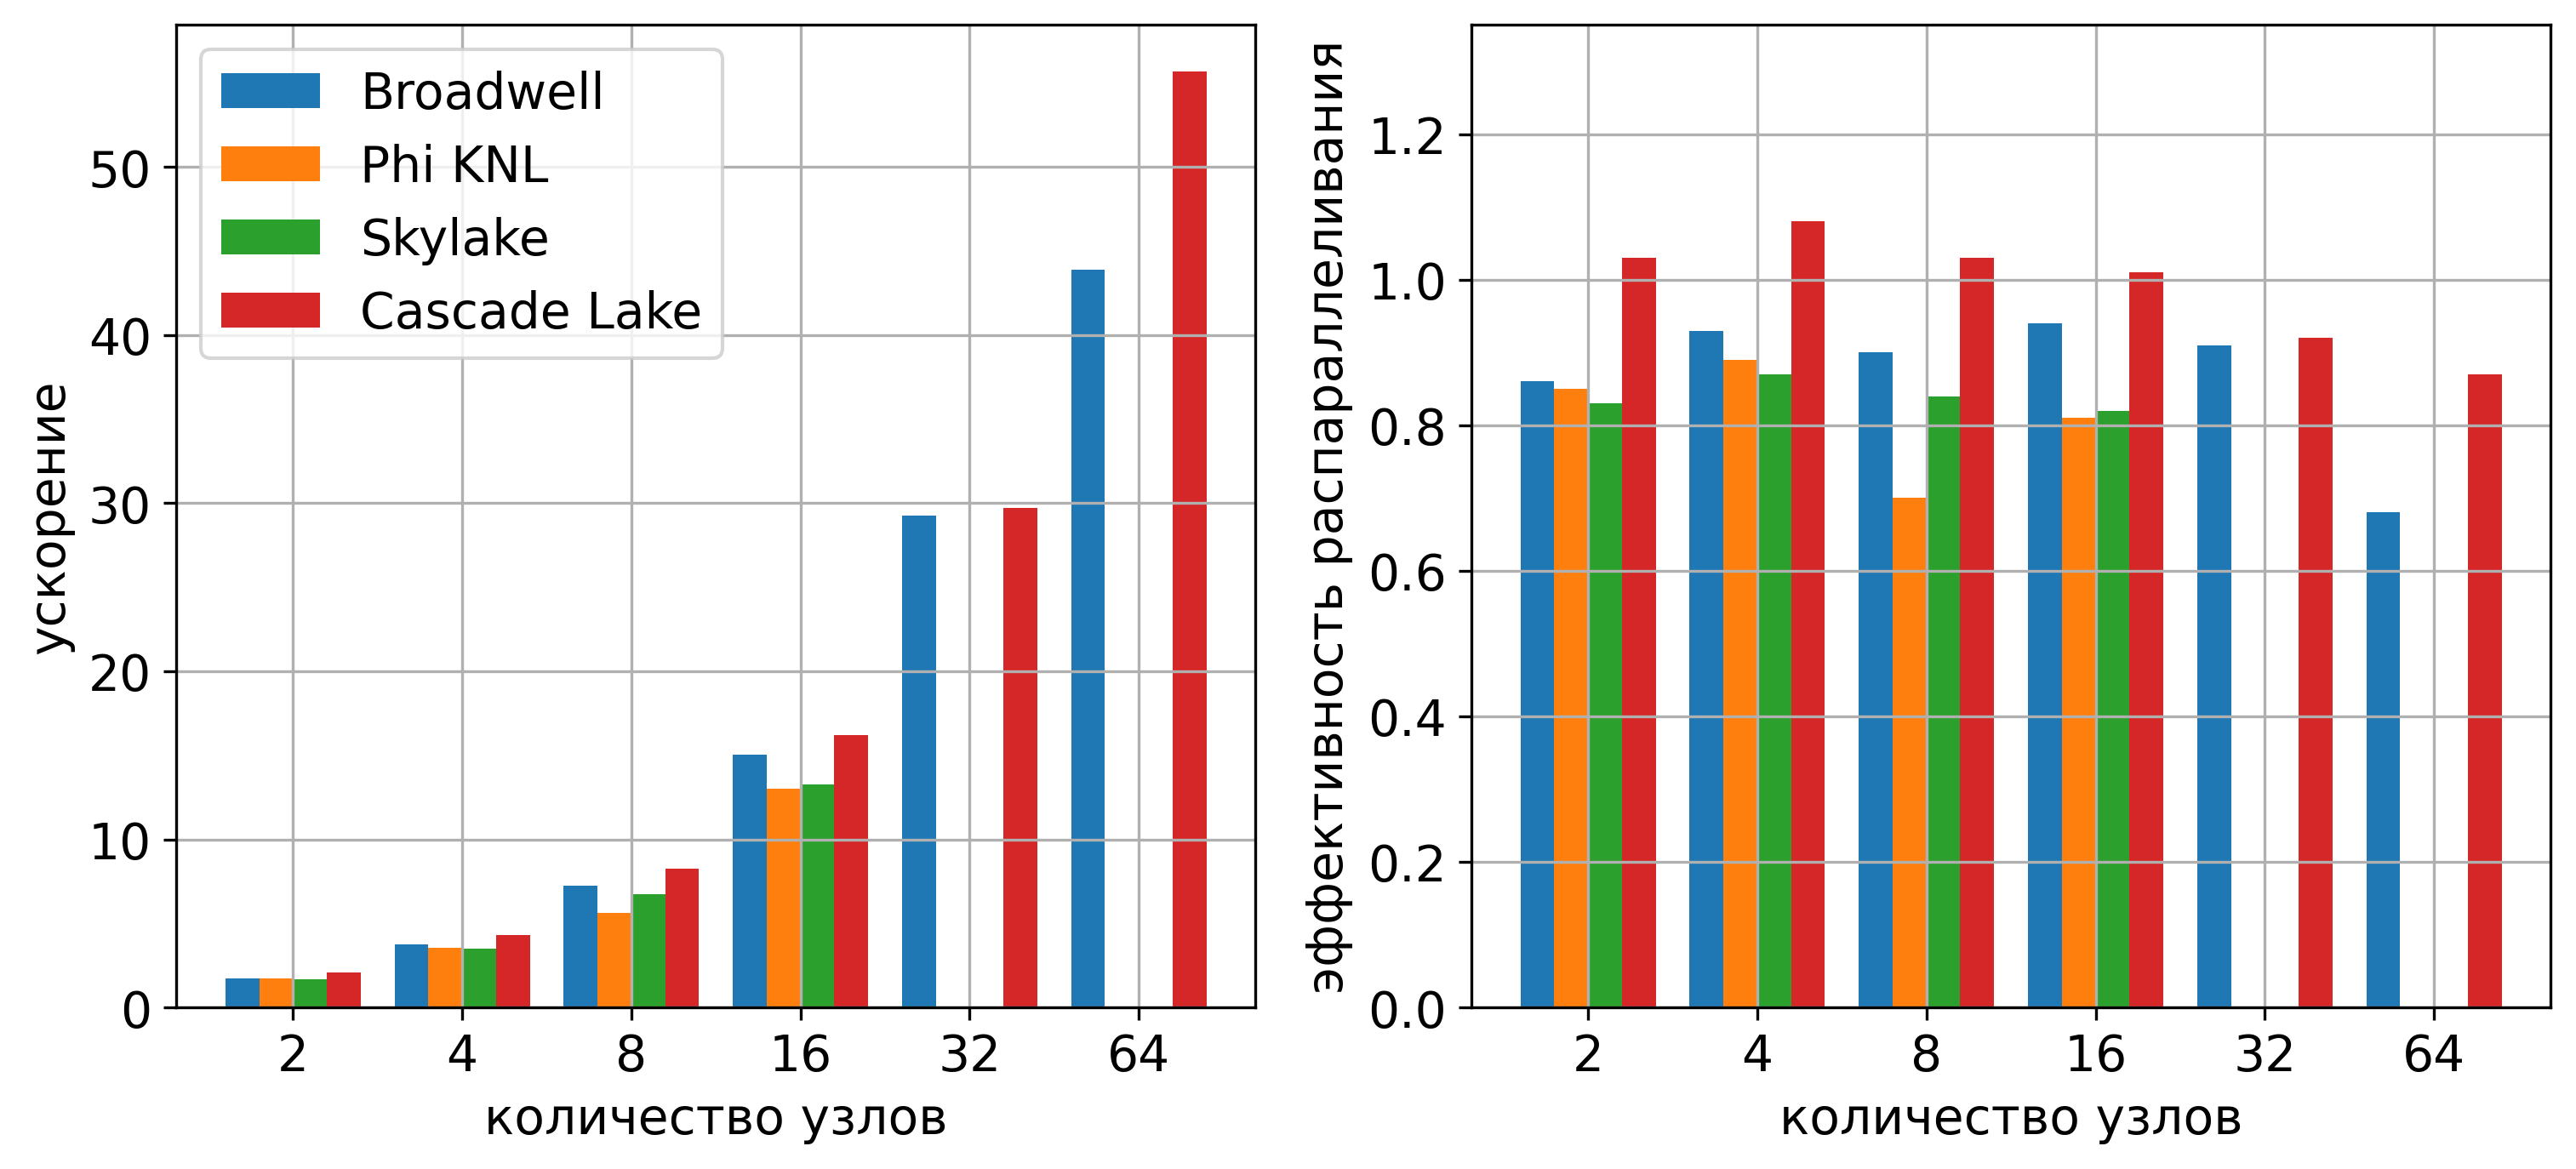
\includegraphics[width=1.0\textwidth]{fig/par_surf_2in1_big.png}
\singlespacing
\caption{Масштабирование расчетов на суперкомпьютере МВС-10П.}
\label{fig:text_2_scaling_speedup_eff}
\end{figure}

В завершении раздела представлен эксперимент по замеру ускорения и эффективности распараллеливания задачи расчета ледообразования на поверхностной неструктурированной расчетной сетке с использованием метода иерархического деления доменов пополам со сглаживанием границ между доменами (рис.~\ref{fig:text_2_scaling_speedup_eff}).
Замеры производились на сегментах суперкомпьютера, состоящих из вычислительных узлов, базирующихся на микропроцессорах Intel Xeon.

%----------------------------------

В разделе~4.4 рассматриваются вопросы распараллеливания вычислений на поверхностной неструктурированной сетке на общей памяти.

Рассматривается проблема устранения конфликтов по данным при распараллеливании конечно-объемных численных методов на поверхностной расчетной сетке.
Конфликты по данным возникают при параллельной обработке перетекания потоков между ячейками.
Рассматривается два подхода к устранению конфликтов.
В качестве первого подхода рассматривается использование директивы \texttt{\#pragma omp atomic} при доступе к элементам данных, по которым возможно возникновение конфликтов.
В качестве второго подхода рассматривается реберная раскраска дуального графа расчетной сетки, с помощью которой множество ребер разбивается на подмножества без конфликтов.
Приводятся алгоритмы реберной раскраски дуального графа поверхностной неструктурированной расчетной сетки в 5 и 4 цвета с линейной сложностью по количеству ребер, а также квадратичный алгоритм раскраски в 3 цвета, основанный на исследованиях раскрасок плоских графов\footnote[2]{С.В.~Курапов, М.В.~Давидовский, А.В.~Толок. Визуальный алгоритм раскраски плоских графов. // Научная визуализация, 2018, Т.~10, №~3, С.~1-33, doi:~10.26583/sv.10.3.01}.
Численные эксперименты показали, что метод устранения конфликтов с помощью реберной раскраски дуального графа приводит к существенному ускорению расчетов на большом количестве потоков.

В разделе рассматривается сравнение эффективности распараллеливания скалярных и векторных вычислений (газодинамический решатель) на общей памяти для вычислительных узлов на базы микропроцессоров Intel (Phi KNL, Skylake, Cascade Lake).

\begin{figure}[ht]
\centering
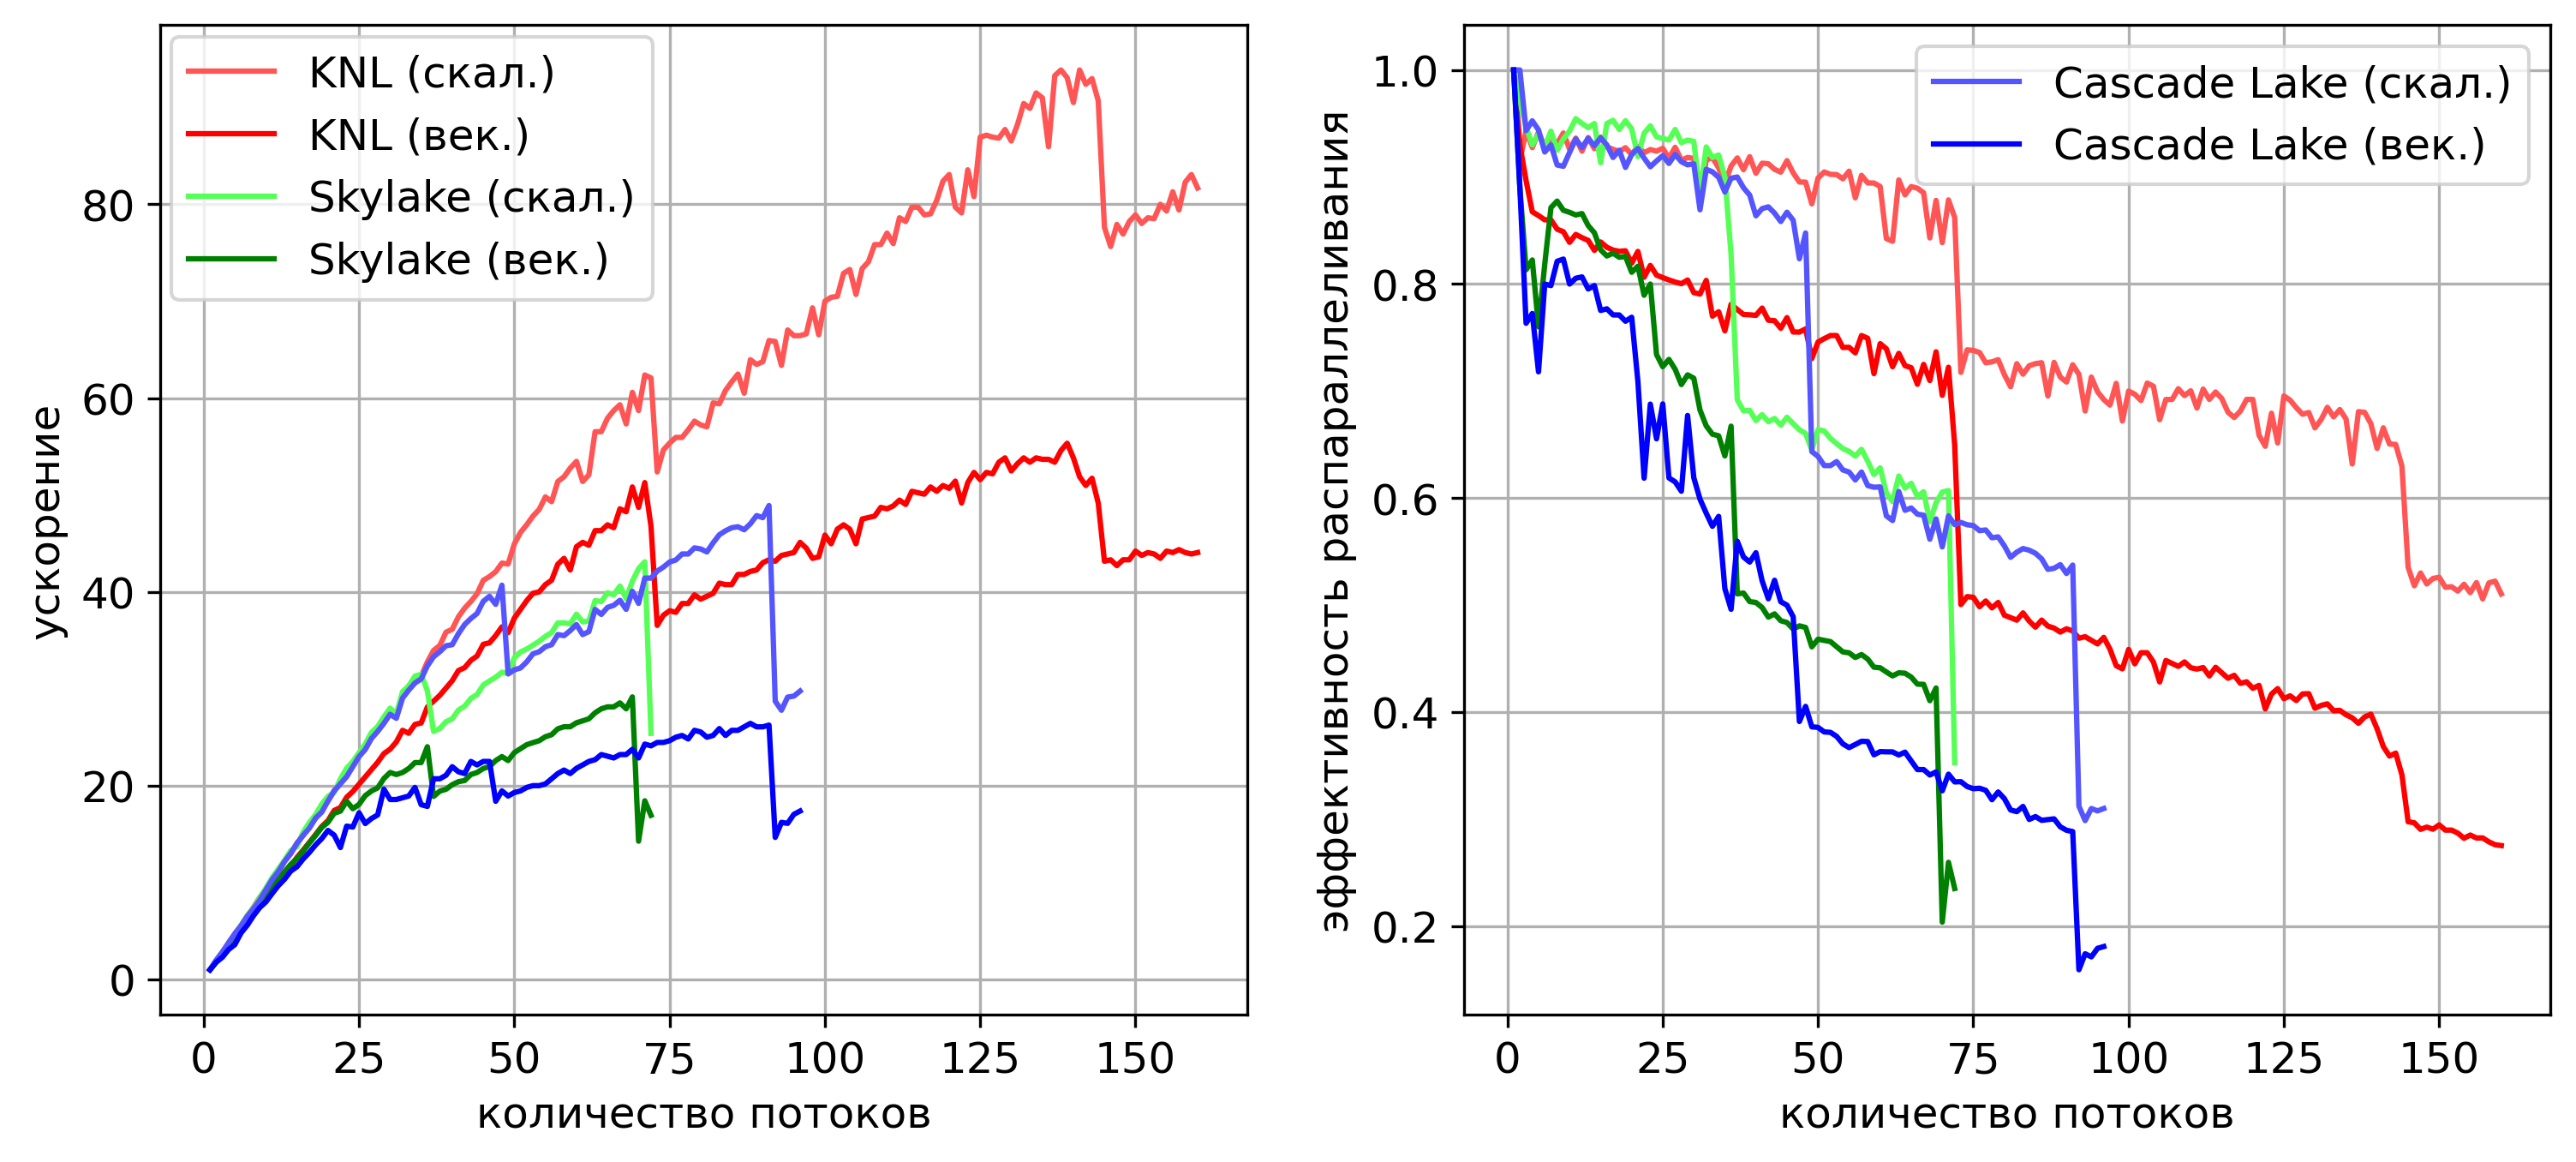
\includegraphics[width=1.0\textwidth]{./fig/par_openmp_scalar_vec_chart_big.png}
\singlespacing
\caption{Графики ускорения и эффективности распараллеливания скалярных и векторизованных вычислений.}
\label{fig:text_3_omp2}
\end{figure}

На рис.~\ref{fig:text_3_omp2} слева представлены графики ускорения скалярной и векторной версии газодинамического решателя на 1-160 потоках.
Для каждого вычислительного узла явно просматриваются отрезки квазилинейного ускорения, которые завершаются провалами.
Длина этих отрезков совпадает с количеством ядер в узле, а провалы обусловлены конкуренцией за аппаратные ресурсы.
Для всех узлов ускорение близко к линейному до тех пор, пока каждый поток запущен на своем ядре.
Из графиков эффективности распараллеливания видно, что эффективность распараллеливания векторных версий кода примерно вдвое ниже эффективности распараллеливания скалярных версий.
Это говорит о целесообразности векторизации программного кода при достижении ускорения от векторизации хотя бы в два раза.

%----------------------------------

Приведены выводы к главе.
Предложенная архитектура блочно-структу\-рированной расчетной сетки с поддержкой дробления блоков.
Проанализированы различные алгоритмы распределения вычислительной нагрузки между вычислительными процессами, сделан вывод о целесообразности применения дробления блоков при проведении вычислений на блочно-структурированных сетках.
Предложенный алгоритм распределения блоков по вычислительным процессам с использованием дробления блоков позволяет добиться распределения с низким показателем неравномерности $D$ при небольшом количестве дроблений блоков $\sigma$.
Предложенный алгоритм сглаживания границ между доменами при декомпозиции поверхностной неструктурированной расчетной сетки позволяет найти точное решение, снизив длины границ примерно на 10\%.
С помощью алгоритмов реберной раскраски дуального графа поверхностной неструктурированной расчетной сетки можно избежать конфликтов по данным при проведении конечно-объемных расчетов на поверхностной расчетной сетке.
Результаты экспериментов по масштабированию скалярных и векторных вычислений на общей памяти показали, что векторизация вычислений оправлана при достижении ускорения хотя бы вдвое по сравнению со скарярным кодом.

%===================================================================================================

\textbf{Пятая глава} посвящена задаче разработки методов векторизации программного кода и методики повышения производительности вычислений с помощью векторизации вычислений.
Приведенные в этой главе методы векторизации могут быть применены для повышения производительности вычислений, проводимых как на поверхностных, так и на объемных расчетных сетках.
Векторизация является оптимизацией распараллеливания вычислений на уровне инструкций и способна кратно увеличить производительность приложений.
Набор векторных инструкций AVX-512 обладает рядом особенностей и позволяет векторизовать сложный программный контекст с обилием операций передачи управления, гнездами циклов и вызовами функций.
Для оценки эффективности векторизации используются понятия \textit{ширина векторизации} $w = v/t$ ($v$ -- размер векторного регистра, $t$ -- размер типа расчетных данных), \textit{ускорение} $s_{vec} = T/T_v$ ($T$ -- время выполнения скалярной версии кода, $T_v$ -- время выполнения векторизованной версии кода), \textit{эффективность} $e_{vec} = s_{vec}/w$, а также \textit{логическое ускорение} $s_{vec}^{*} = L/L_v$ ($L$ -- количество выполненных инструкций в скалярном коде, $L_v$ -- количество выполненных аналогичных им векторных инструкций в векторном коде), \textit{логическая эффективность} $e_{vec}^{*} = s_{vec}^{*}/w$.

%----------------------------------

В разделе~5.1 приведено описание набора векторных инструкций AVX-512, перечислены основные подмножества операций и рассмотрены особенности этого набора.
Основной отличительной чертой этого набора инструкций, позволяющей векторизовать программный контекст со сложным управлением, является возможность выполнения векторных инструкций с использованием \textit{векторных масок}, определяющих индексы элементов, для которых в выходной регистр записывается результат операции.

%----------------------------------

В разделе~5.2 рассматривается векторизация программного кода путем выделения однотипных инструкций и объединения их в векторные аналоги на примере операций с матрицами малой размерности.
На примере матричных операций показано, что от способа выделения однотипных инструкций для объединения в векторные аналоги существенным образом зависит производительность результирующего кода.
Также продемонстрировано, что низкая \textit{плотность векторных масок} (доля единичных битов в маске) в результирующем коде негативно сказывается на производительности.

%----------------------------------

В разделе~5.3 вводится понятие \textit{плоского цикла} как удобного контекста для векторизации вычислений, что делает его предпочтительной формой компоновки программного кода для успешного автоматического применения векторизации оптимизирующим компилятором.
Идея плоского цикла состоит в объединении $w$ экземпляров \textit{скалярного блока} в единый \textit{векторный блок}, состоящий из аналогичных векторных инструкций, где $w$ -- ширина векторизации.
Так $w$ экземпляров скалярного блока $block(x, y) \rightarrow r$ со скалярными входными данными $x$, $y$ и скалярным результатом $r$ могут быть объединены в векторный блок $BLOCK(X, Y) \rightarrow R$ с векторными входными данными $X$, $Y$ и векторным результатом $R$.
В качестве плоского цикла будем рассматривать цикл \texttt{for (int i = 0; i < w; ++i)}, к которому предъявляются следующие требования.
На $i$-ой итерации все обращения к данным на запись имеют вид \texttt{a[i]}, а обращения к данным на чтение либо имеют вид \texttt{a[i]}, либо являются чтением скаляров.
Все массивы данных, обращение к которым на $i$-ой итерации цикла имеет вид \texttt{a[i]}, выровнены в памяти на размер вектора.
В цикле отсутствуют межитерационные зависимости.
Без ограничения общности можно считать, что плоский цикл содержит произвольное количество итераций $n$, так как с помощью расщепления цикла по индуктивной переменной он может быть разбит на $\lfloor n/w \rfloor$ циклов с $w$ итерациями и возможно еще один с меньшим количеством итераций (\textit{эпилог}).
Цикл, в котором нарушаются некоторые другие из приведенных требований, называется \textit{квазиплоским}.

%\begin{figure}[!ht]
%\centering
%\includegraphics[width=1.0\textwidth]{./fig/vec_avx512_semantic_table.pdf}
%\singlespacing
%\caption{Инструкции AVX-512 для работы с вещественными числами и их семантика. $A$, $B$, $R$ -- векторные регистры, $P$, $Q$ -- векторные маски.}
%\label{fig:vec_avx512_semantic_table}
%\end{figure}

Плоский цикл является удобным для векторизации программным контекстом и зачастую может быть заменем на векторный блок (или на несколько соседних векторных блоков в случае произвольного количества итераций $n > w$), а логика работы многих векторных инструкций может быть представлена в виде плоского цикла и записана в предикатной форме.
В качестве примера обсуждается применение автоматической векторизации к программному коду, представленному в виде композиции плоских циклов (на примере реализации газодинамического решателя), а также демонстрируется деградация производительности на квазиплоских циклах.
Для приведения программного кода к виду плоских циклов применяется организация данных в виде набора массивов, а также расщепление циклов по константному условию для сокращения количества операций передачи управления внутри цикла.

%\begin{figure}[!ht]
%\centering
%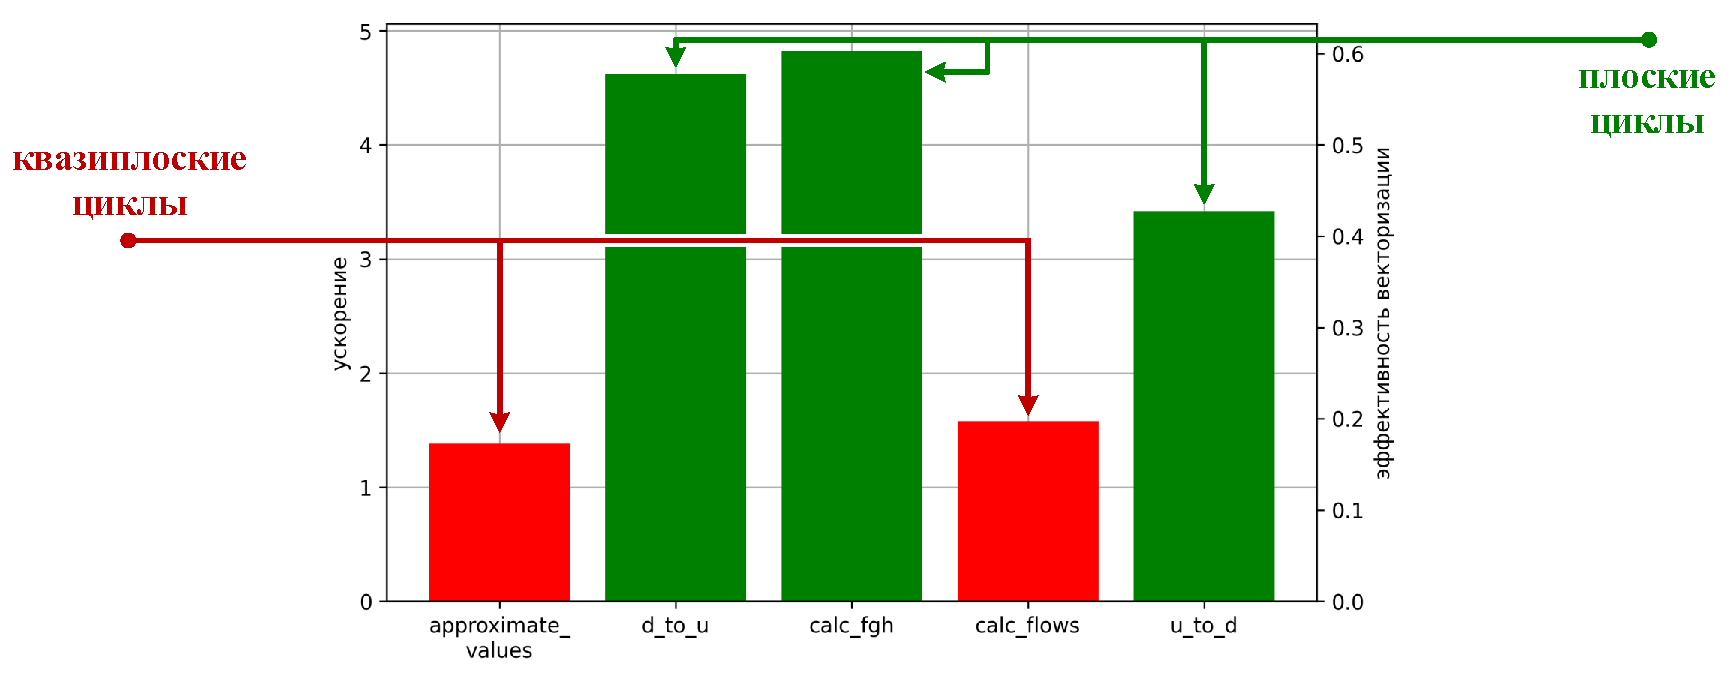
\includegraphics[width=0.7\textwidth]{./fig/vec_diagram_ibm_functions.pdf}
%\singlespacing
%\caption{Диаграмма $s_{vec}$ и $e_{vec}$ функций газодинамического решателя.}
%\label{fig:vec_diagram_ibm_functions}
%\end{figure}

%----------------------------------

В разделе~5.4 рассматривается оптимизация \textit{выноса маловероятного региона из плоского цикла}.
Инструкции передачи управления не имеют векторных аналогов, их наличие в коде является основной причиной низкой эффективности векторизации.
Большинство ориентированных на векторизацию оптимизаций направлены на упрощение управления в векторизуемом коде. 
Оптимизация выноса маловероятного региона заключается в сохранении условий входа в этот регион во временный массив и удалении его из основного цикла.
Основной цикл, свободный от удаленного региона, может быть успешно векторизован, а вынесенный маловероятный регион может быть обработан в отдельном цикле согласно сохраненным условиям.
Оптимизация применима в том случае, если все выходы из выносимого региона являются переходами на следующую итерацию плоского цикла или выходами из него.

%----------------------------------

В разделе~5.5 рассматривается оптимизация \textit{слияния путей исполнения по условию} внутри плоского цикла с помощью постановки операций из параллельных скалярных блоков под предикаты этих блоков, трансформирующиеся при векторизации в векторные маски.
Приводятся аналитические оценки логической эффективности векторизации плоского цикла, в котором два скалярных блока (с вероятностями $p$ и $1 - p$ и длинами $\frac{\alpha}{\alpha + 1}$ и $\frac{1}{\alpha + 1}$ соответственно) сливаются по условию в случае независимости условий с разных итераций плоского цикла.
Рассматриваются два варианта векторного кода -- без проверки маски векторного блока на пустоту перед его выполнением и с проверкой (рис.~\ref{fig:vec_ifconv_nocheck_check}).

\begin{figure}[!ht]
\centering
\begin{tabular}{ll}
\begin{subfigure}{0.45\textwidth}\centering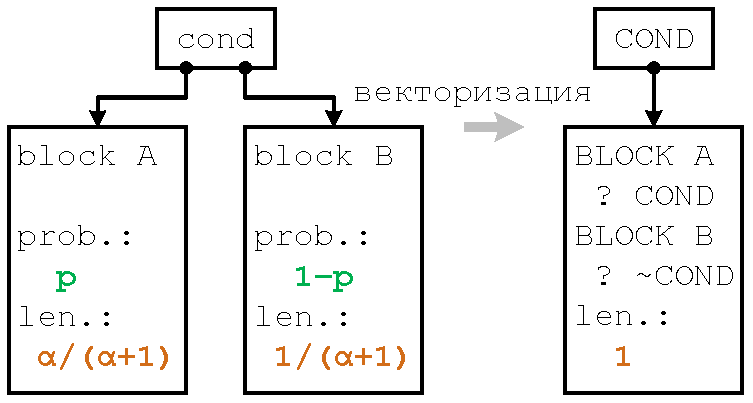
\includegraphics[width=0.85\columnwidth]{./fig/vec_ifconv_nocheck_big.pdf}\caption{простое слияние}\end{subfigure} &
\begin{subfigure}{0.45\textwidth}\centering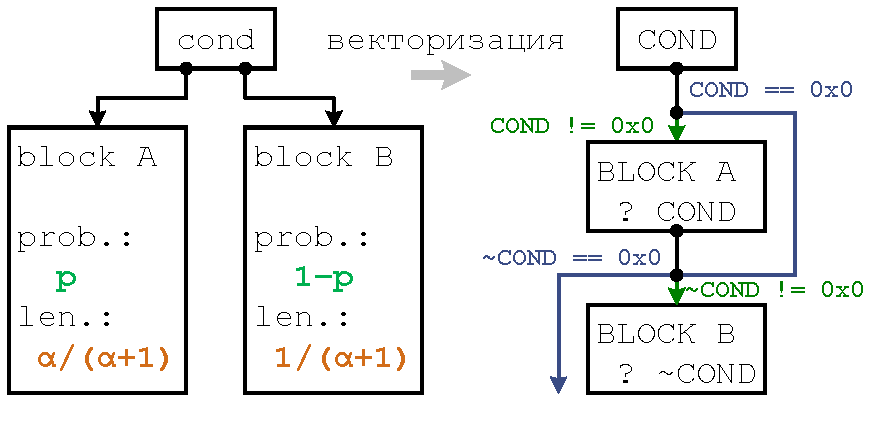
\includegraphics[width=0.85\columnwidth]{./fig/vec_ifconv_check_big.pdf}\caption{слияние с проверкой масок}\end{subfigure}
\end{tabular}
\singlespacing
\caption{Схема векторизации со слиянием блоков.}
\label{fig:vec_ifconv_nocheck_check}
\end{figure}

Выводятся зависимости логической эффективности векторизации от вероятности перехода $p$
\begin{equation*}
e_{vec}^{*} =
	\begin{cases}
		p\left(\frac{\alpha - 1}{\alpha + 1}\right) + \left(\frac{1}{\alpha + 1}\right), & \text{простое слияние} \\
		\frac{ p(\alpha - 1) + 1 }{\left(1 - (1 - p)^w\right) \alpha + (1 - p^w)},       & \text{с проверкой масок на пустоту}
	\end{cases}
\end{equation*}
из чего сделан вывод о низкой эффективности векторизации при слиянии большого количества путей исполнения внутри плоского цикла.

%\begin{figure}[!ht]
%\centering
%\begin{tabular}{ll}
%\begin{subfigure}{0.45\textwidth}\centering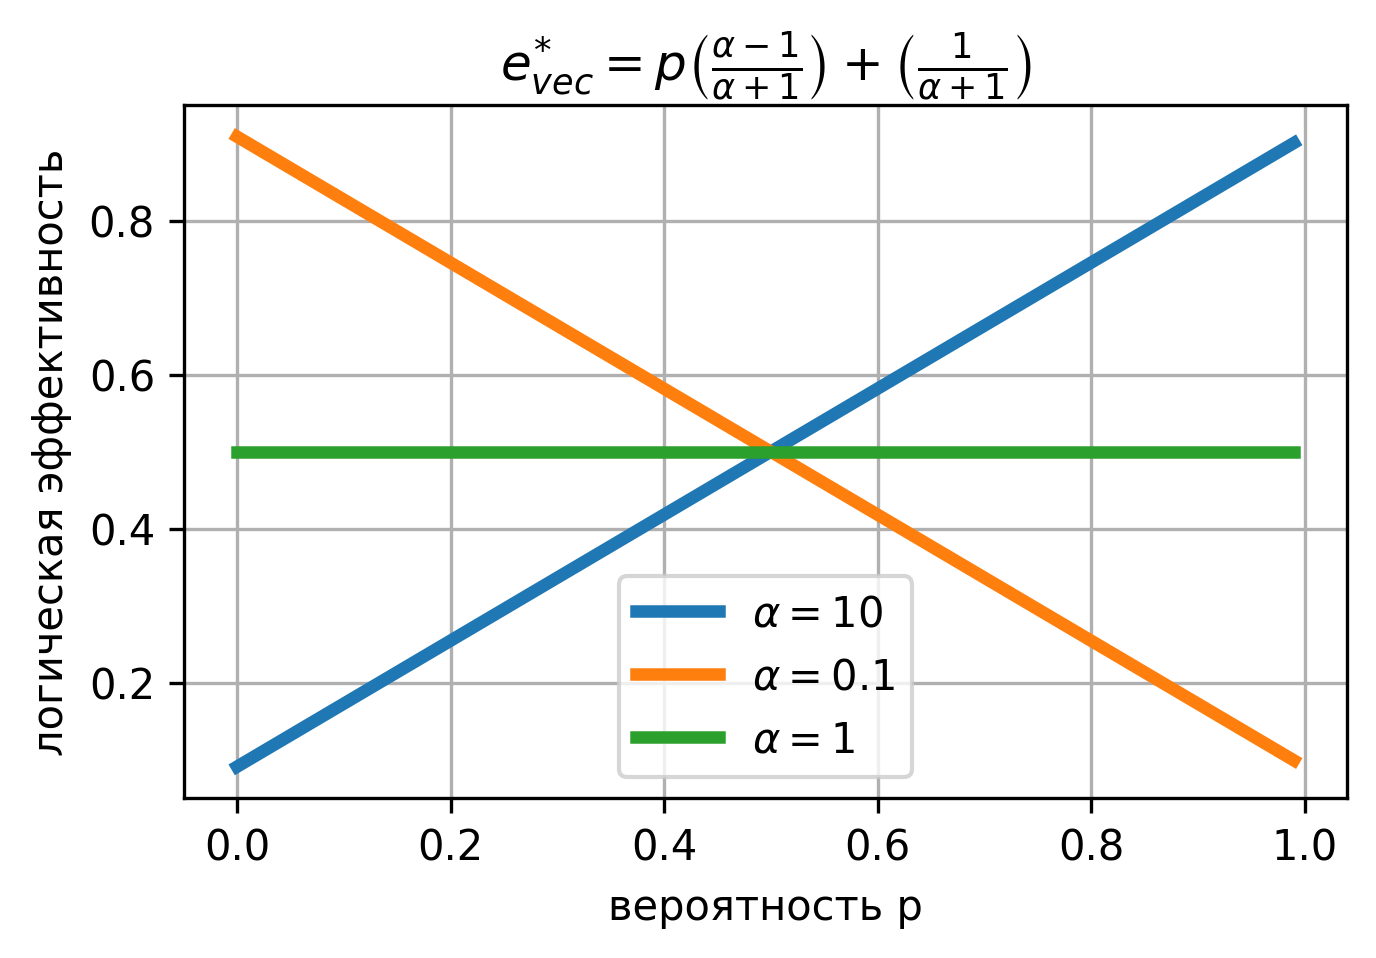
\includegraphics[width=0.85\columnwidth]{./fig/vec_ifconv_nocheck_chart.png}\caption{простое слияние}\end{subfigure} &
%\begin{subfigure}{0.45\textwidth}\centering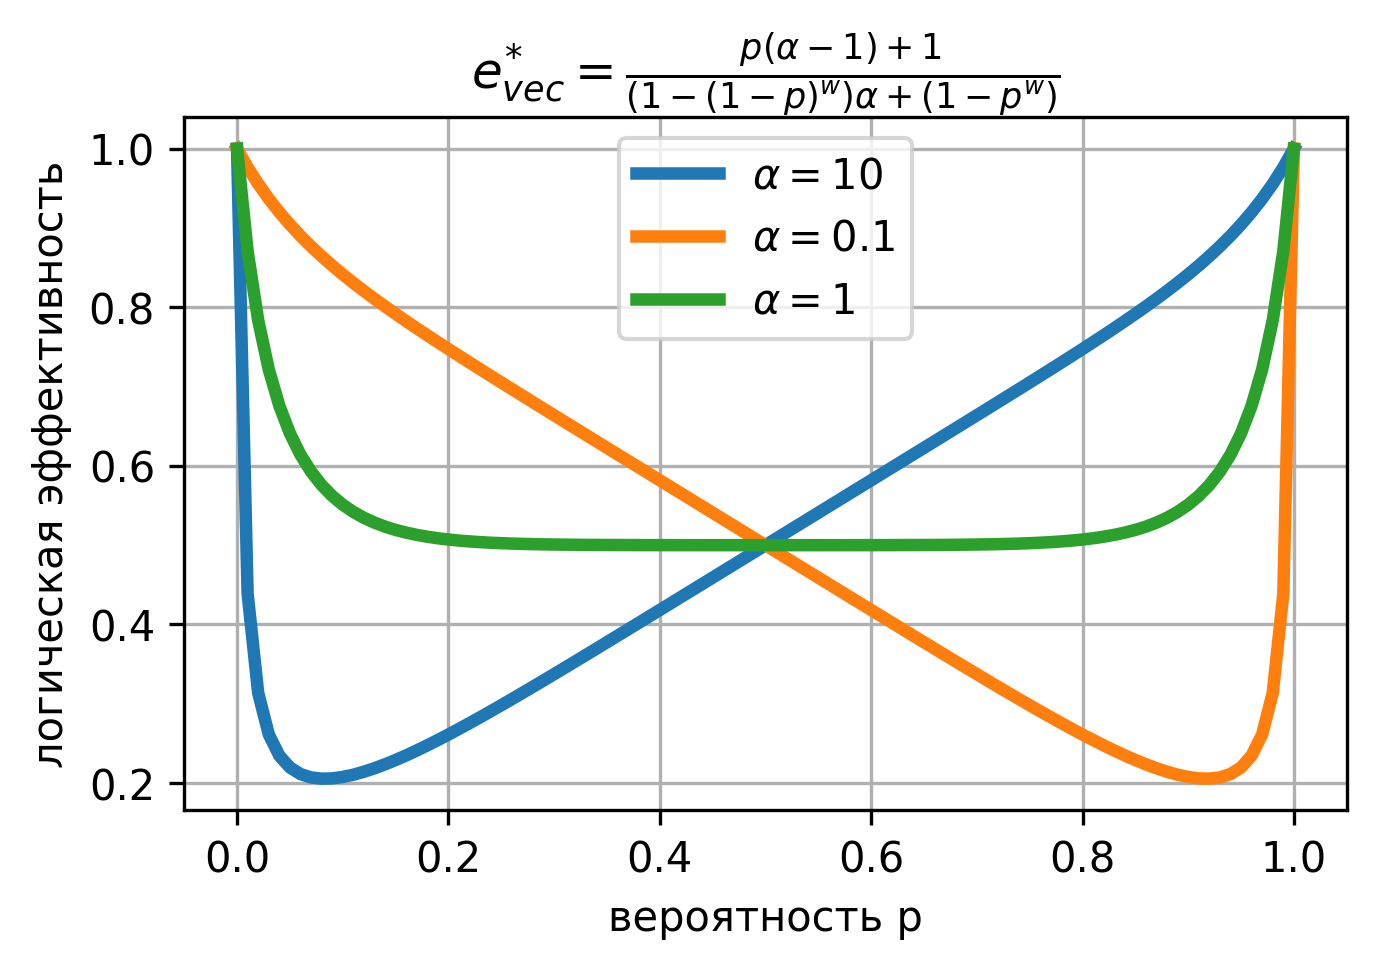
\includegraphics[width=0.85\columnwidth]{./fig/vec_ifconv_check_chart.png}\caption{слияние с проверкой масок}\end{subfigure}
%\end{tabular}
%\singlespacing
%\caption{Графики зависимости $e_{vec}^{*}$ от вероятности перехода $p$ при разных $\alpha$.}
%\label{fig:vec_charts_nocheck_check}
%\end{figure}

%\begin{figure}[!ht]
%\centering
%\begin{tabular}{ll}
%\begin{subfigure}{0.45\textwidth}\centering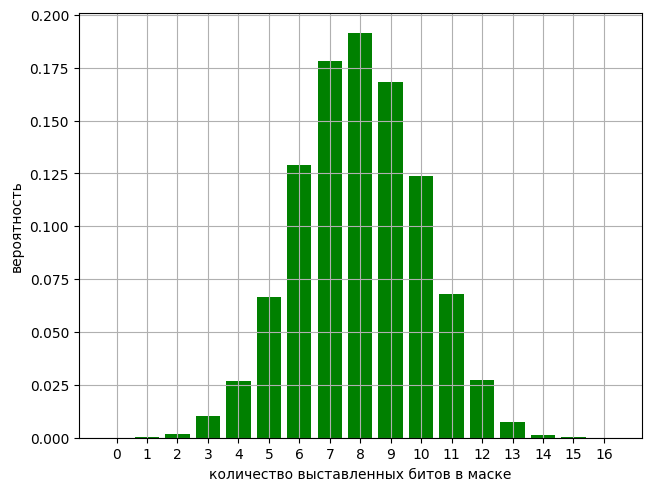
\includegraphics[width=0.85\columnwidth]{./fig/vec_mask_distr_independent_p.png}\caption{независимые условия}\end{subfigure} &
%\begin{subfigure}{0.45\textwidth}\centering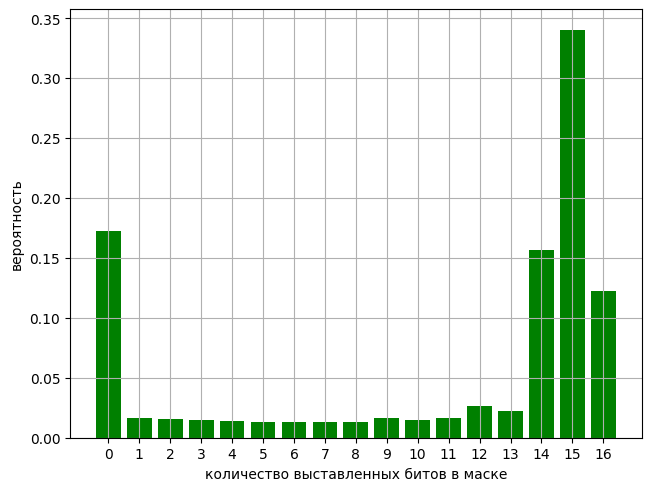
\includegraphics[width=0.85\columnwidth]{./fig/vec_mask_distr_real_p.png}\caption{реальное приложение}\end{subfigure}
%\end{tabular}
%\singlespacing
%\caption{Типовое распределение количества единичных битов в маске.}
%\label{fig:vec_masks_density}
%\end{figure}

Отмечается, что проверка векторной маски на пустоту перед выполнением векторного блока зачастую оправдана, так как на реальных приложениях пустые маски встречаются достаточно часто.
Это связано с тем, что на расчетных приложениях характерно медленное изменение величин при переходе между итерациями плоского цикла, что влечет за собой медленное изменение условий, что в свою очередь приводит к частому возникновению пустых и полных масок при векторизации.

%----------------------------------

В разделе~5.6 рассматривается повышение плотности масок векторного кода с помощью \textit{объединения масок} и \textit{комбинирования масок} соседних векторных блоков.
Так как в общем случае без учета комбинированных операций $L = w \sum_{c \in C_v}{\rho(m(c))}$ ($C_v$ -- множество векторных инструкций в векторном коде, $m(c)$ -- маска инструкции, $\rho(m)$ -- плотность маски), то для повышения эффективности векторизации требуется повышение плостности векторных масок.
Если два соседних векторных блока \texttt{block(in\_data\_1)} $\rightarrow$ \texttt{out\_data\_1} и \texttt{block(in\_data\_2)} $\rightarrow$ \texttt{out\_data\_2} выполняются под непересекающимися масками \texttt{(mask\_1 \& mask\_2) == 0x0}, то вычисления в этих блоках можно объединить.
Вместо их последовательного выполнения можно объединить входные данные \texttt{in\_data\_1} и \texttt{in\_data\_2} с помощью слияния по маске \texttt{in\_data = blend(mask\_1, in\_data\_2, in\_data\_1}), после чего выполнить тот же блок вычислений под маской \texttt{mask\_1 | mask\_2}.
Ввиду отсутствия пересечения векторных масок в результирующих выходных данных \texttt{out\_data} будут содержаться как необходимые элементы данных \texttt{out\_data\_1}, так и необходимые элементы данных \texttt{out\_data\_2} (рис.~\ref{fig:vec_unite_masks}).
Комбинирование масок позволяет объединить вычисления в соседних блоках в случае пересечения векторных масок, если сумма их плотностей не превышает единицу.

\begin{figure}[ht]
\centering
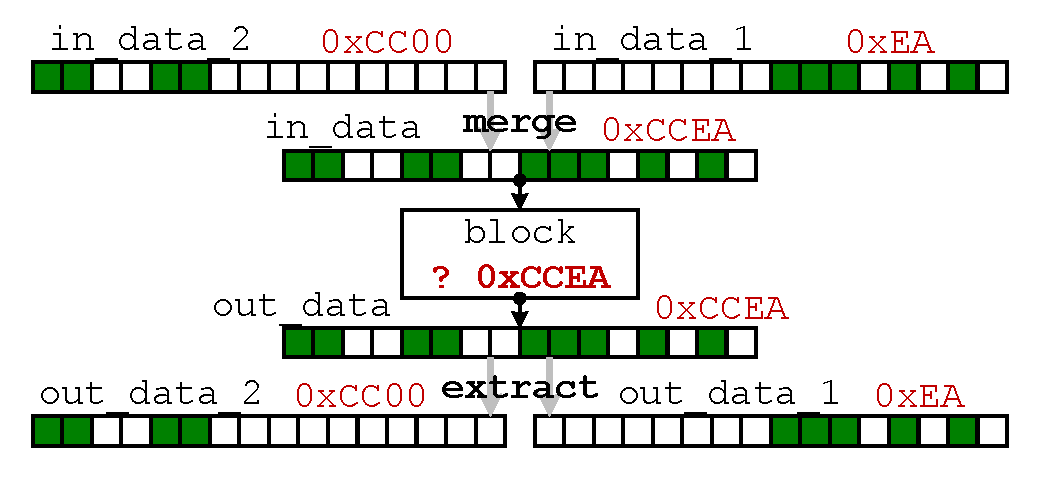
\includegraphics[width=0.6\textwidth]{./fig/vec_masks_union_big.pdf}
\singlespacing
\caption{Схема вычислений с объединением масок двух векторных блоков.}
\label{fig:vec_unite_masks}
\end{figure}

%----------------------------------

В разделе~5.7 проводится анализ программного контекста, в котором тело плоского цикла само содержит циклы или гнезда циклов.
На рис.~\ref{fig:vec_flat_loop_nest} представлена схема векторизации плоского цикла, в теле которого содержится внутренний цикл (\textit{структура <<плоский цикл / внутренний цикл>>}).

\begin{figure}[!ht]
\centering
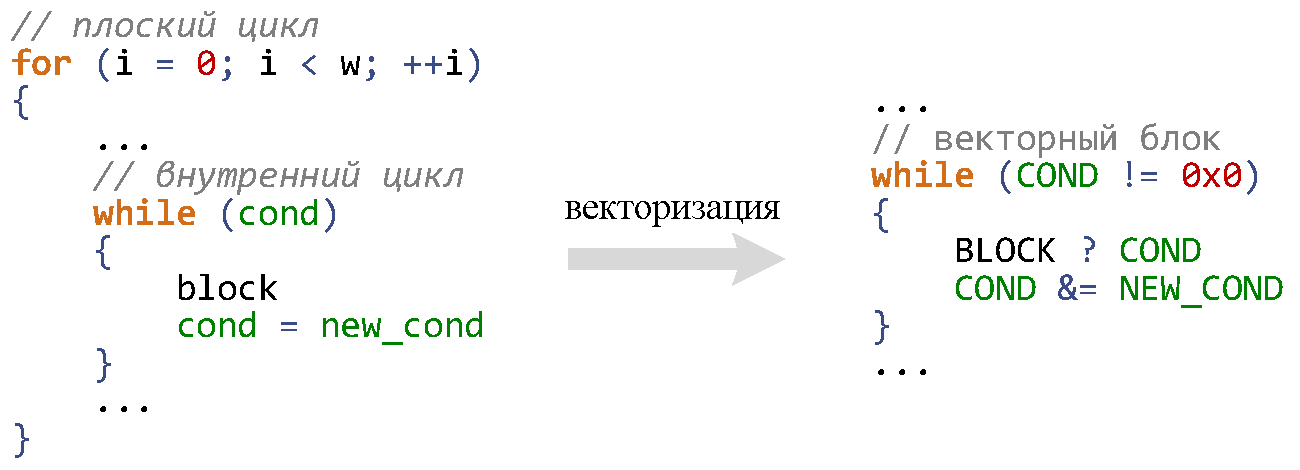
\includegraphics[width=0.7\textwidth]{./fig/vec_flat_loop_nest.pdf}
\singlespacing
\caption{Схема векторизации стуктуры <<плоский цикл / вложенный цикл>>.}
\label{fig:vec_flat_loop_nest}
\end{figure}

При выполнении векторизации тело внутреннего цикла $block$, выполняемое по условию $cond$, переводится в векторный блок $BLOCK$, инструкции которого выполняются под маской $COND$, которая постепенно истощается пока не станет равной \texttt{0x0}.
При этом выполняется соотношение $I_v = \max_{i = 0}^{w - 1}{I(i)}$, где $I(i)$ -- количество итераций внутреннего цикла на $i$-ой итерации плоского цикла, $I_v$ -- количество итераций внутреннего цикла в векторизованной версии.
Эффективность векторизации рассматриваемого программного кода зависит от характера измерения условия $cond$ (и соответственно функции $I(i)$) при переходе между итерациями плоского цикла.
В терминах количества итераций справедлива следующая лемма.

\textbf{Лемма.} \textit{При векторизации структуры <<плоский цикл / внутренний цикл>> верна априорная оценка $e_{vec}^{*} \le e_{vec}^I$, где $e_{vec}^I = ( \sum_{i = 0}^{w - 1}{I(i)} ) / (I_v w)$.
При этом, если выполняется соотношение $I_v - \min_{i = 0}^{w - 1}{I(i)} \le \epsilon$, то $e_{vec}^I \ge 1 - \frac{\epsilon}{I_v}$.}

Отдельно рассматриваются различные виды внутреннего цикла, и анализируется влияние его характера на эффективность векторизации.

В разделе~5.7.1 рассматривается внутренний \textit{цикл с фиксированным количеством итераций}, то есть условие выхода из которого является константным для векторизуемого плоского цикла.
В этом случае $e_{vec}^I = 1$, при векторизации условие выхода из внутреннего цикла переносится в векторизованный код в неизменном виде.

\begin{figure}[!ht]
\centering
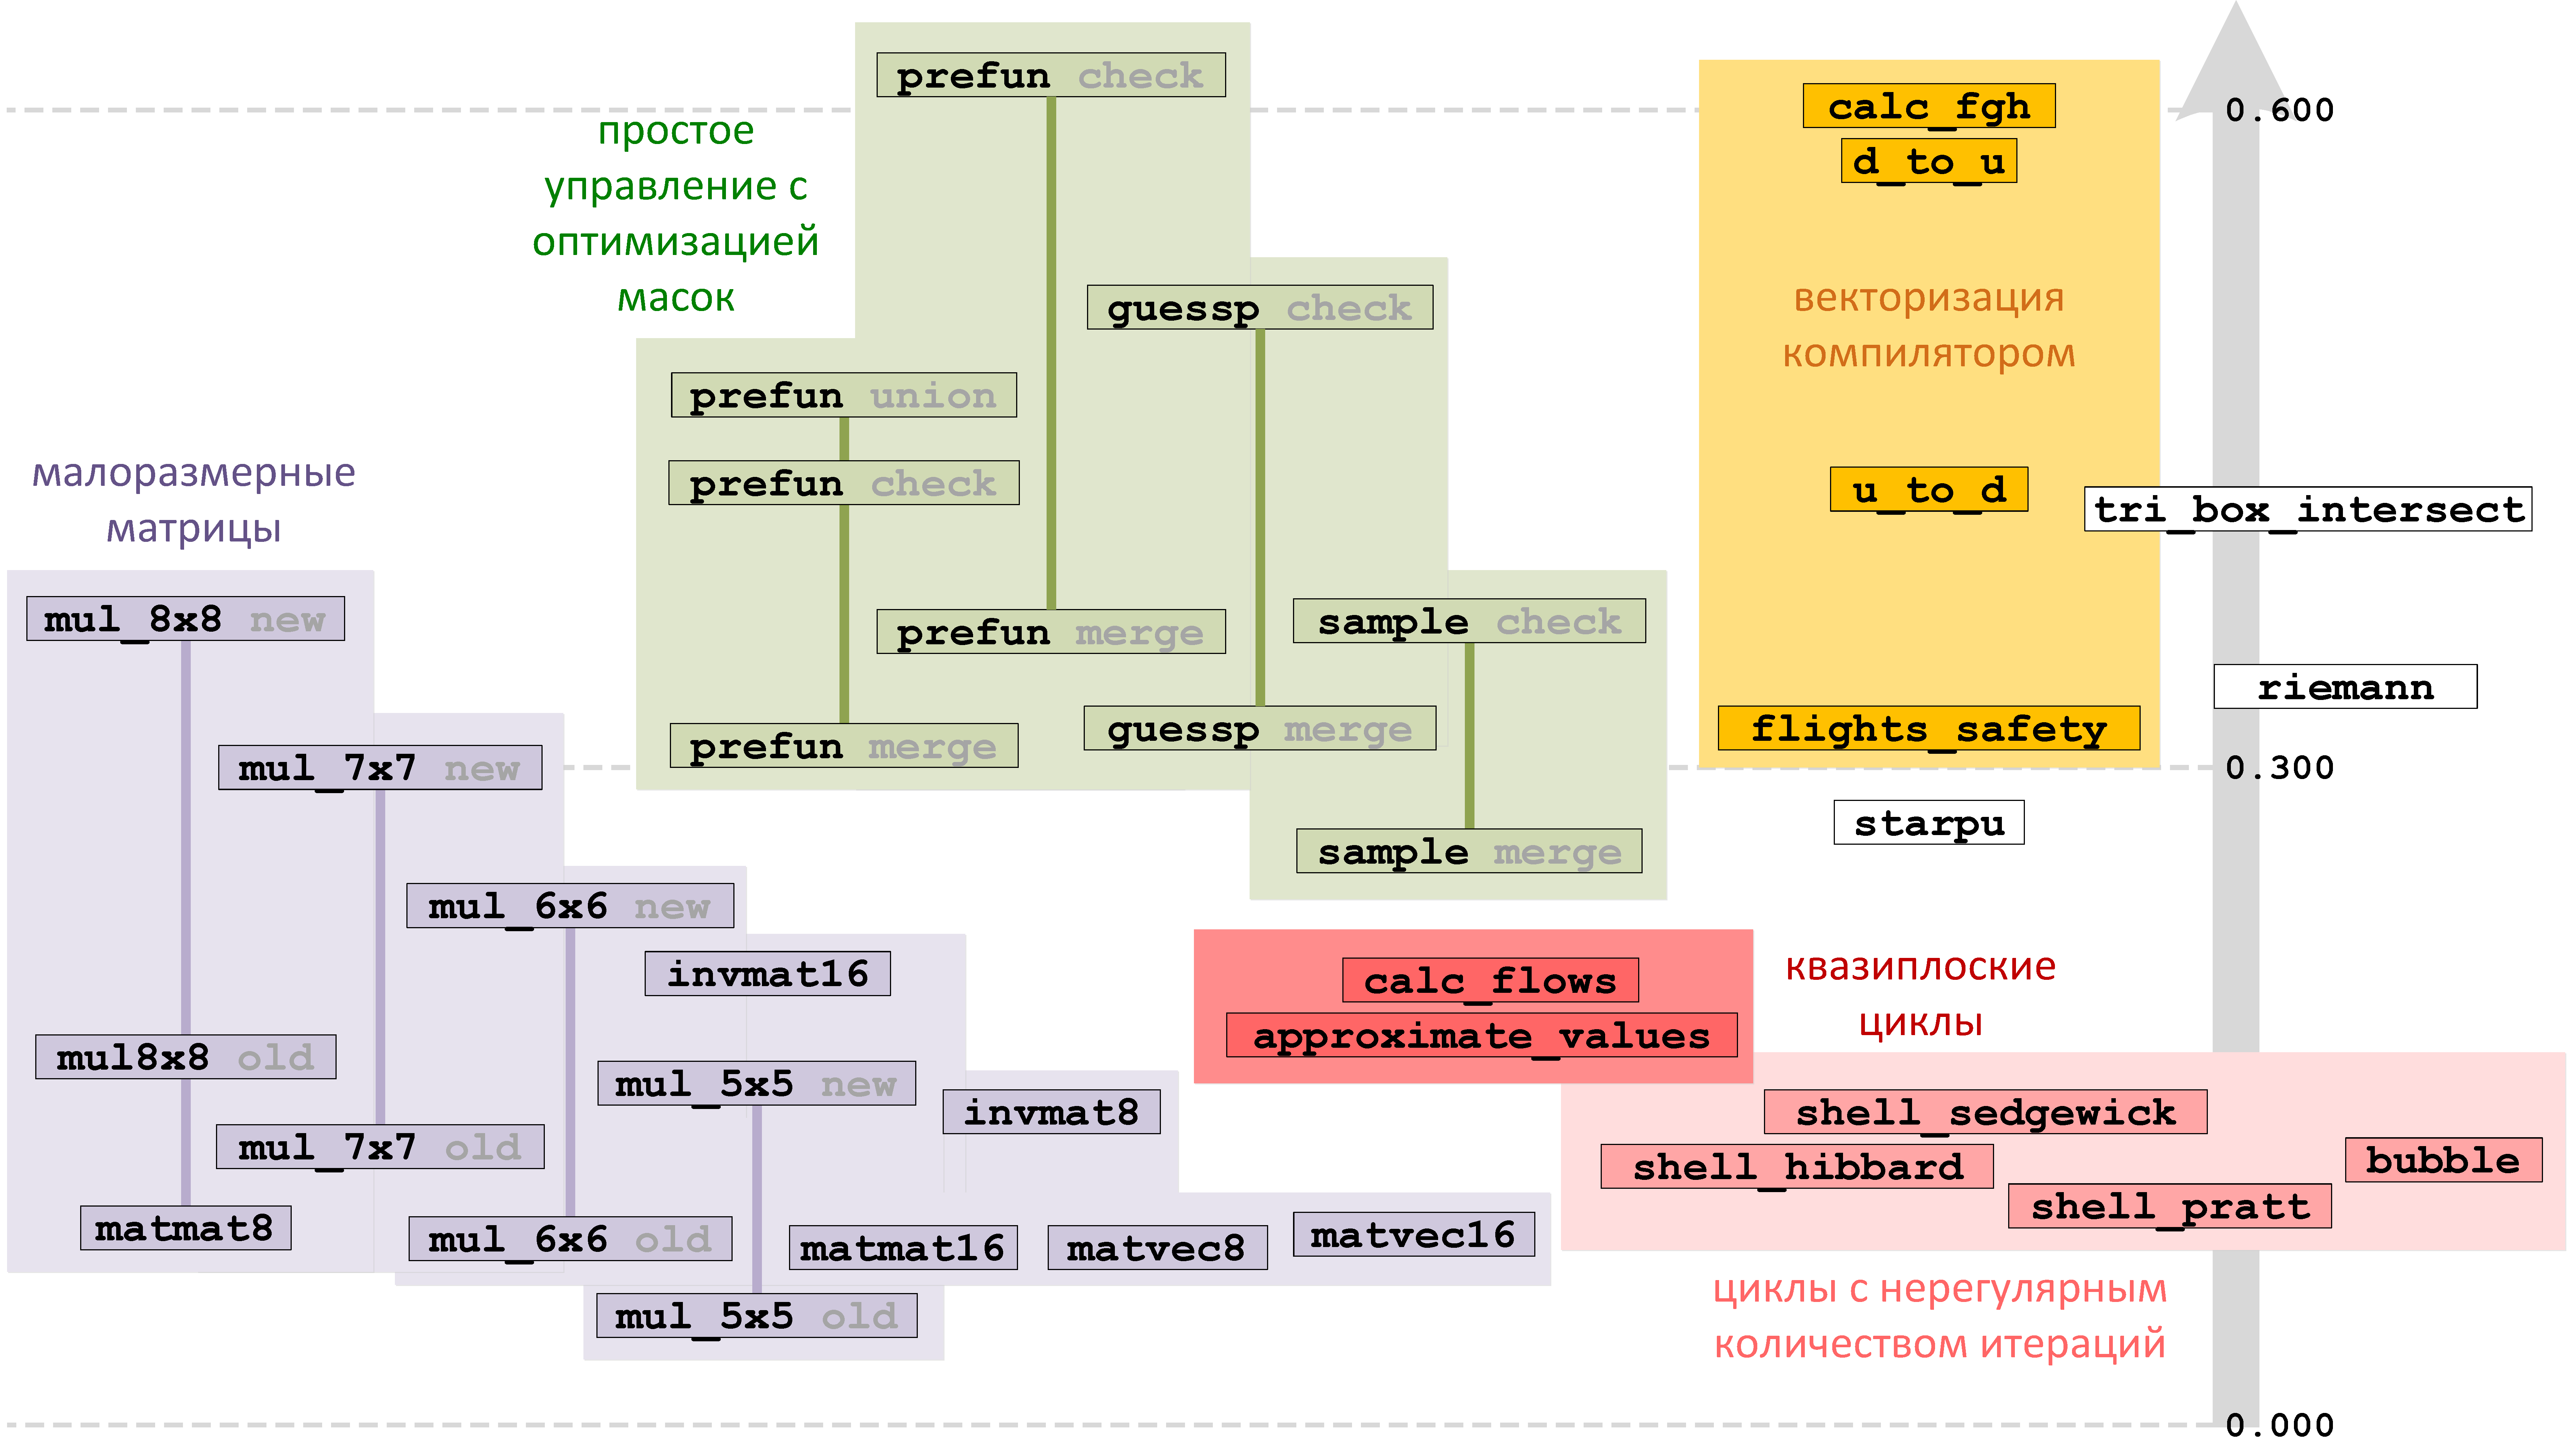
\includegraphics[width=1.0\textwidth]{./fig/vec_fin_map.pdf}
\singlespacing
\caption{Карта эффективности векторизации.}
\label{fig:vec_fin_map}
\end{figure}

В разделе~5.7.2 рассматривается внутренний \textit{цикл с непостоянным количеством итераций}, то есть в котором условие выхода из цикла зависит от номера итерации векторизуемого плоского цикла, но изменяется медленно (значение коэффициента $\epsilon$ мало).
При векторизации условие выхода из внутреннего цикла трансформируется в векторную маску выполнения тела, и внутренний цикл продолжает исполняться до тех пор, пока эта векторная маска не истощится.
Основной причиной потери производительности при векторизации такого программного контекста является выполнение итераций внутреннего цикла под маской низкой плотности.

В разделах~5.7.3 и 5.7.4 рассматривается вещественный и целочисленный программный контекст в котором внутренний цикл характеризуется как \textit{цикл с нерегулярным количеством итераций} (значение коэффициента $\epsilon$ сравнимо с величиной $I_v$).
При векторизации такого программного контекста плотность маски выполнения внутреннего цикла является крайне низкой, что приводит к наиболее серьезной потере производительности. 

%----------------------------------

В выводах из главы приводится общая карта рассмотренного в главе векторизованного программного контекста, представленная на рис.~\ref{fig:vec_fin_map}.
Из карты делается вывод, что наиболее неудобным программным контекстом для векторизации являются гнезда циклов с нерегулярным количеством итераций, а также квазиплоские циклы c дополнительной косвенностью при обращении в память, невыровненностью данных и другими нарушениями требований, предъявляемых к плоским циклам.
Наиболее удобным контекстом для векторизации являются плоские циклы с простым управлением и применением проверок и объединения масок.
Рассмотренные в главе преобразования, направленные на упрощение управления в плоском цикле и повышение плотности масок в векторном коде приводят к повышению эффективности векторизации и могут быть использованы для ускорения высокопроизводительных приложений. 

%---------------------------------------------------------------------------------------------------

\textbf{В заключении} приведены выводы диссертации.
Разработан и реализован метод окрестностей перестроения поверхностной расчетной сетки, который позволяет сглаживать дефекты расчетной сетки и обеспечивает стабильность выполнения расчетов по моделированию обледенения.
Разработаны и реализованы методы удаления самопересечений поверхностной расчетной сетки, которые позволяют избежать аварийной остановки расчетов по моделированию обледенения, продолжение которых невозможно при возникновении этого критического дефекта.
Разработан и реализован метод погруженной границы для сопряжения с объемной расчетной сеткой, позволяющий выполнять расчет поля скоростей без необходимости создания согласованной расчетной сетки в пространстве.
Разработаны и реазованы методы повышения производительности параллельных вычислений на объемных и поверхностных расчетных сетках в моделях распараллеливания с передачей сообщений и на общей памяти.
Разработана методика и ряд методов повышения производительности вычислений с помощью векторизации програмного кода.
Таким образом, разработан и реализован ряд научно-технических решений для повышения производительности вычислений при моделировании обледенения на поверхностной расчетной сетке с изменяемой геометрией.

\section*{Основные публикации по теме диссертации}

\begin{enumerate}[noitemsep,topsep=0pt,parsep=0pt,partopsep=0pt]
\item Рыбаков~А.~А. Декомпозиция расчетной сетки с помощью генетического алгоритма. // Программные продукты и системы, 2025, Т.~38, №~2, С.~337-344. doi:~10.15827/0236-235X.150.337-344
\item Рыбаков~А.~А. Векторизация циклов с условными операциями с помощью комбинирования векторных масок. // Современные информационные технологии и ИТ-образование, 2024, Т.~20, №~3, С.~563-572. doi:~10.25559/SITITO.020.202403.563-572
\item Гуличева~А.~А., Рыбаков~А.~А. Реберная раскраска кубического графа в задаче распараллелирования расчетов на неструктурированной поверхностной расчетной сетке. // Программные продукты и системы, 2024, Т.~37, №~3, С.~374-383. doi:~10.15827/0236-235X.142.374-383
\item Рыбаков~А.~А., Швиндт~А.~Н. Создание инструментария для векторизации тела плоского цикла с помощью векторных инструкций AVX-512. // Программные продукты и системы, 2023, Т.~36, №~4, С.~561-572. doi:~10.15827/0236-235X.142.561-572
\item Рыбаков~А.~А. Геометрическое перестроение расчетной сетки с помощью общей огибающей семейства сфер в задаче ледообразования. // Современные информационные технологии и ИТ-образование, 2023, Т.~19, №~2, С.~282-291. doi:~10.25559/SITITO.019.202302.282-291
\item Рыбаков~А.~А., Мещеряков~А.~О. Векторизация трехмерного метода погруженных границ для повышения эффективности расчетов на микропроцессорах Intel. // Программные продукты и системы, 2023, Т.~36, №~1, С.~130-143. doi:~10.15827/0236-235X.141.130-143
\item Meshcheryakov~A.~O., Rybakov~A.~A. Evolution of the surface computational mesh in the ice accretion process. // Lobachevskii Journal of Mathematics, 2023, Vol.~44, No.~11, P.~361-378. doi:~10.1134/S1995080223110367
\item Freylekhman~S.~A., Rybakov~A.~A. Self-intersections elimination for unstruc\-tured surface computational meshes. // Lobachevskii Journal of Mathema\-tics, 2022, Vol.~43, No.~10, P.~2846-2852. doi:~10.1134/S1995080222130133
\item Рыбаков~А.~А. Векторизация программного кода, содержащего маловероятные регионы, в задачах вычислительной геометрии. // Современные информационные технологии и ИТ-образование, 2022, Т.~18, №~1, С.~28-38. doi:~10.25559/SITITO.18.202201.28-38
\item Багров~А.~Д., Рыбаков~А.~А. Сглаживание границ между доменами поверхностной расчетной сетки. // Современные информационные технологии и ИТ-образование, 2021, Т.~17, №~2, C.~265-274. \\ doi:~10.25559/SITITO.17.202102.265-274
\item Shabanov~B.~M., Rybakov~A.~A., Shumilin~S.~S., Vorobyov~M.~Yu. Scaling of supercomputer calculations on unstructered surface computational meshes. // Lobachevskii Journal of Mathematics, 2021, Vol.~42, No.~11, P.~2571-2579. doi:~10.1134/S1995080221110202
\item Рыбаков~А.~А., Чопорняк~А.~Д. Декомпозиция поверхностной неструктурированной расчетной сетки для масштабирования вычислений на суперкомпьютере. // Современные информационные технологии и ИТ-образование, 2020, Т.~16, №~4, С.~851-861. \\ doi:~10.25559/SITITO.16.202004.851-861
\item Рыбаков~А.~А. Метод погруженной границы с использованием фиктивных ячеек в трехмерной постановке. // Современные информационные технологии и ИТ-образование, 2020, Т.~16, №~2, С.~321-330. \\ doi:~10.25559/SITITO.16.202002.321-330
\item Savin~G.~I., Shabanov~B.~M., Rybakov~A.~A., Shumilin~S.~S. Vectorization of flat loops of arbitrary structure using instructions AVX-512. // Lobachevskii Journal of Mathematics, 2020, Vol.~41, No.~12, P.~2575-2592. \\ doi:~10.1134/S1995080220120331
\item Рыбаков~А.~А., Шумилин~С.~С. Исследование эффективности векторизации гнезд циклов с нерегулярным числом итераций. // Программные системы: Теория и приложения, 2019, Т.~10, №~4(43), С.~77-96. doi:~10.25209/2079-3316-2019-10-4-77-96
\item Рыбаков~А.~А., Шумилин~С.~С. Векторизация римановского решателя с использованием набора инструкций AVX-512. // Программные системы: Теория и приложения, 2019, Т.~10, №~3(42), С.~59-80. \\ doi:~10.25209/2079-3316-2019-10-3-59-80
\item Rybakov~A.~A., Shumilin~S.~S. Approximate methods of the surface mesh deformation in two-dimensional case. // Lobachevskii Journal of Mathem\-atics, 2019, Vol.~40, No.~11, P.~1848-1852. doi:~10.1134/S1995080219110258
\item Savin~G.~I., Benderskiy~L.~A., Lyubimov~D.~A., Rybakov~A.~A. RANS/ILES method optimization for effective calculations on supercomputer. // Loba\-chevskii Journal of Mathematics, 2019, Vol.~40, No.~5, P.~566-573. \\ doi:~10.1134/S1995080219050172
\item Shabanov~B.~M., Rybakov~A.~A., Shumilin~S.~S. Vectorization of high-performance scientific calculations using AVX-512 instruction set. // Loba\-chevskii Journal of Mathematics, 2019, Vol.~40, No.~5, P.~580-598. \\ doi:~10.1134/S1995080219050196
\item Бендерский~Л.~А., Рыбаков~А.~А., Шумилин~С.~С. Векторизация перемножения малоразмерных матриц специального вида с использованием инструкций AVX-512. // Современные информационные технологии и ИТ-образование, 2018, Т.~14, №~3, С.~594-602. \\ doi:~10.25559/SITITO.14.201803.594-602
\item Бендерский~Л.~А., Лещев~С.~А., Рыбаков~А.~А. Векторизация операций над матрицами малой размерности для процессора Intel Xeon Phi Knights Landing. // Современные информационные технологии и ИТ-образование, 2018, Т.~14, №~1, С.~73-90. \\ doi:~10.25559/SITITO.14.201801.073-090
\item Рыбаков~А.~А. Оптимизация задачи об определении конфликтов с опасными зонами движения летательных аппаратов для выполнения на Intel Xeon Phi. // Программные продукты и системы, 2017, Т.~30, №~3, С.~524-528. doi:~10.15827/0236-235X.030.3.524-528
\item Рыбаков~А.~А. Внутреннее представление и механизм межпроцессного обмена для блочно-структурированной сетки при выполнении расчетов на суперкомпьютере. // Программные системы: Теория и приложения, 2017, Т.~8, №~1(32), С.~121-134. doi:~10.25209/2079-3316-2017-8-1-121-134
\item Рыбаков~А.~А. Распределение вычислительной нагрузки между узлами суперкомпьютерного кластера при расчетах задач газовой динамики с дроблением расчетной сетки. // Современные информационные технологии и ИТ-образование, 2016, Т.~12, №~2, С.~101-107.
\end{enumerate}

% Другие статьи (Труды НИИСИ, сборник конференции).
%\begin{enumerate}[noitemsep,topsep=0pt,parsep=0pt,partopsep=0pt]
%\item Рыбаков~А.~А., Телегин~П.~Н., Шабанов~Б.~М. Проблемы векторизации гнезд циклов с использованием инструкций AVX-512. // Электронный научный журнал: Программные продукты, системы и алгоритмы, 2018, №~3, С.~1-11.
%\item Рыбаков~А.~А. Распределение вычислительной нагрузки между узлами гетерогенного вычислительного кластера. // Электронный научный журнал: Программные продукты, системы и алгоритмы, 2018, №~1, C.~26-32.
%\item Шабанов~Б.~М., Рыбаков~А.~А., Чопорняк~А.~Д. Оптимизации, применяемые к графу потока управления программы для повышения эффективности векторизации плоских циклов. // Труды НИИСИ РАН, 2021, Т.~11, №~2, С.~11-19.
%\item Воробьев~М.~Ю., Рыбаков~А.~А., Никсон Муганда Очара. Исследование масштабируемости плотных параллельных вычислений на микропроцессорах Intel. // Инжиниринг предприятий и управление знаниями (ИП\&УЗ-2020). Сборник научных трудов XXIII Международной научной конференции, 2020, С.~45-52.
%\item Воробьев~М.~Ю., Рыбаков~А.~А., Чопорняк~А.~Д. Сравнение стратегий распараллеливания векторизованного римановского решателя с помощью OpenMP для микропроцессора Intel Xeon Phi KNL. // Труды НИИСИ РАН, 2020, Т.~10, №~5-6, С.~113-119.
%\item Рыбаков~А.~А., Чопорняк~А.~Д. Повышение производительности векторного кода с помощью мониторинга плотности масок в векторных инструкциях. // Труды НИИСИ РАН, 2020, Т.~10, №~4, С.~40-47.
%\item Рыбаков~А.~А. Векторизация нахождения пересечения объемной и поверхностной сеток для микропроцессоров с поддержкой AVX-512. // Труды НИИСИ РАН, 2019, Т.~9, №~5, С.~5-14.
%\item Rybakov~A.~A., Shumilin~S.~S. Vectorization of the Riemann solver using the AVX-512 instruction set. // Program Systems: Theory and Applications, 2019, Vol.~10, №~3(42), P.~41-58.
%\item Рыбаков~А.~А., Шумилин~С.~С. Векторизация сильно разветвленного управления с помощью инструкций AVX-512. // Труды НИИСИ РАН, 2018, Т.~8, №~4, С.~114-126.
%\item Бендерский~Л.~А., Любимов~Д.~А., Рыбаков~А.~А. Инструментарий подготовки блочно-структурированной сетки для проведения расчетов методом RANS/ILES. // Труды НИИСИ РАН, 2018, Т.~8, №~4, С.~102-106.
%\item Бендерский~Л.~А., Любимов~Д.~А., Рыбаков~А.~А. Анализ эффективности масштабирования при расчетах высокоскоростных турбулентных течений на суперкомпьютере RANS/ILES методом высокого разрешения. // Труды НИИСИ РАН, 2017, Т.~7, №~4, С.~32-40.
%\end{enumerate}

\end{document}
